%%%%%%%%%%%%%%%%%%%%%%%%%%%%%%%%%%%%%%%%%%%%%%%%%%%%%%%%%%%%%%%%%%%%%
%%                                                                 %%
%% Please do not use \input{...} to include other tex files.       %%
%% Submit your LaTeX manuscript as one .tex document.              %%
%%                                                                 %%
%% All additional figures and files should be attached             %%
%% separately and not embedded in the \TeX\ document itself.       %%
%%                                                                 %%
%%%%%%%%%%%%%%%%%%%%%%%%%%%%%%%%%%%%%%%%%%%%%%%%%%%%%%%%%%%%%%%%%%%%%

%%\documentclass[referee,sn-basic]{sn-jnl}% referee option is meant for double line spacing

%%=======================================================%%
%% to print line numbers in the margin use lineno option %%
%%=======================================================%%

%%\documentclass[lineno,sn-basic]{sn-jnl}% Basic Springer Nature Reference Style/Chemistry Reference Style

%%======================================================%%
%% to compile with pdflatex/xelatex use pdflatex option %%
%%======================================================%%

%%\documentclass[pdflatex,sn-basic]{sn-jnl}% Basic Springer Nature Reference Style/Chemistry Reference Style

%%\documentclass[sn-basic]{sn-jnl}% Basic Springer Nature Reference Style/Chemistry Reference Style
\documentclass[pdflatex,sn-mathphys]{sn-jnl}% Math and Physical Sciences Reference Style
%%\documentclass[sn-aps]{sn-jnl}% American Physical Society (APS) Reference Style
%%\documentclass[sn-vancouver]{sn-jnl}% Vancouver Reference Style
%%\documentclass[sn-apa]{sn-jnl}% APA Reference Style
%%\documentclass[sn-chicago]{sn-jnl}% Chicago-based Humanities Reference Style
%%\documentclass[sn-standardnature]{sn-jnl}% Standard Nature Portfolio Reference Style
%%\documentclass[default]{sn-jnl}% Default
%%\documentclass[default,iicol]{sn-jnl}% Default with double column layout

%%%% Standard Packages
%%<additional latex packages if required can be included here>
%%%%

%%%%%=============================================================================%%%%
%%%%  Remarks: This template is provided to aid authors with the preparation
%%%%  of original research articles intended for submission to journals published 
%%%%  by Springer Nature. The guidance has been prepared in partnership with 
%%%%  production teams to conform to Springer Nature technical requirements. 
%%%%  Editorial and presentation requirements differ among journal portfolios and 
%%%%  research disciplines. You may find sections in this template are irrelevant 
%%%%  to your work and are empowered to omit any such section if allowed by the 
%%%%  journal you intend to submit to. The submission guidelines and policies 
%%%%  of the journal take precedence. A detailed User Manual is available in the 
%%%%  template package for technical guidance.
%%%%%=============================================================================%%%%

\jyear{2021}%

%% as per the requirement new theorem styles can be included as shown below
\theoremstyle{thmstyleone}%
\newtheorem{theorem}{Theorem}%  meant for continuous numbers
%%\newtheorem{theorem}{Theorem}[section]% meant for sectionwise numbers
%% optional argument [theorem] produces theorem numbering sequence instead of independent numbers for Proposition
\newtheorem{proposition}[theorem]{Proposition}% 
%%\newtheorem{proposition}{Proposition}% to get separate numbers for theorem and proposition etc.

\theoremstyle{thmstyletwo}%
\newtheorem{example}{Example}%
\newtheorem{remark}{Remark}%

\theoremstyle{thmstylethree}%
\newtheorem{definition}{Definition}%

\raggedbottom
%%\unnumbered% uncomment this for unnumbered level heads


\usepackage{caption}
\usepackage{subcaption}
% \usepackage{graphicx}
\usepackage{placeins}

\begin{document}

\title[Chronic Stress Assessment Based on EEG Signals]{Chronic Stress Assessment Based on EEG Signals: An Empirical Method for EEG Feature Importance}

%%=============================================================%%
%% Prefix	-> \pfx{Dr}
%% GivenName	-> \fnm{Joergen W.}
%% Particle	-> \spfx{van der} -> surname prefix
%% FamilyName	-> \sur{Ploeg}
%% Suffix	-> \sfx{IV}
%% NatureName	-> \tanm{Poet Laureate} -> Title after name
%% Degrees	-> \dgr{MSc, PhD}
%% \author*[1,2]{\pfx{Dr} \fnm{Joergen W.} \spfx{van der} \sur{Ploeg} \sfx{IV} \tanm{Poet Laureate} 
%%                 \dgr{MSc, PhD}}\email{iauthor@gmail.com}
%%=============================================================%%

\author{\fnm{Rattaphong} \sur{Laoharungpisit}}\email{laoharungpisit.r@gmail.com}
\equalcont{These authors contributed equally to this work.}
\author{\fnm{Akraradet} \sur{Sinsamersuk}}\email{akraradets@gmail.com}
\equalcont{These authors contributed equally to this work.}

\author{\fnm{Chaklam} \sur{Silpasuwanchai}}\email{chaklam@ait.ac.th}
\author{\fnm{Matthew} \sur{Dailey}}\email{mdailey@ait.ac.th}
\author{\fnm{Attaphongse} \sur{Taparugssanagorn}}\email{attaphongset@ait.ac.th}
\affil{\orgdiv{Center for Health and Wellness Technologies}, {\orgdiv{School of Engineering and Technology}, \orgname{Asian Institute of Technology}}}
%\orgaddress{\street{Street}, \city{City}, \postcode{100190}, \state{State}, \country{Country}}}
%\affil[2]{\orgdiv{Department}, \orgname{Organization}, \orgaddress{\street{Street}, \city{City}, \postcode{10587}, \state{State}, \country{Country}}}
%\affil[3]{\orgdiv{Department}, \orgname{Organization}, \orgaddress{\street{Street}, \city{City}, \postcode{610101}, \state{State}, \country{Country}}}



% https://www.verywellmind.com/chronic-stress-3145104
\abstract{Chronic stress is a prolonged and constant feeling of stress that could lead to depression and anxiety. It would be useful to have a self-diagnosing tool to help notify individuals before chronic stress becomes unmanageable. EEG analysis has proven effective as a means of human emotion prediction, but studies linking EEG analysis with and chronic stress are limited. To fill this gap, we recorded rest-state EEG and perceived stress scale (PSS) scores for 55 participants. Five frequency bands (delta, theta, alpha, beta, and gamma) and lateral asymmetry between electrode pairs calculated for the alpha and beta bands are extracted as features from the rest-state EEG. A feature selection procedure was performed using a t-tests and feature importance scores based on five classifiers. A RBF SVM achieved a 10-cv score over 0.9 using eight different combinations of frequency bands, electrodes, and asymmetries, namely, $\beta_{f}$, $\text{F3}_{\delta}$, $\text{F4}_{\delta}$, $\text{F3}_{\beta}$, $\text{P4}_{\delta}$, $\text{F3}_{\gamma}$, $\text{P4}_{\theta}$, and $\text{C3}_{\theta}$. This paper shows that data-driven feature selection for EEG signals can yield accurate chronic stress classifiers.}

\keywords{Long-term stress, Chronic stress, Electroencephalography}
%%\pacs[JEL Classification]{D8, H51}

%%\pacs[MSC Classification]{35A01, 65L10, 65L12, 65L20, 65L70}

\maketitle
\section{Introduction} \label{sec1}
Stress is an unavoidable life phenomenon that can generate temporary discomfort as well as long-term consequences. Stress can have damaging effects on the mental health of individuals and can be categorized into acute (short-term) and chronic (long-term) occurrences \cite{Khosrowabadi-2011}. Acute stress is usually not a health risk, but the persistence of stress for a longer duration becomes chronic \cite{Khosrowabadi-2011}, which can lead to a state of depression, anxiety, and other possibly life-threatening issues. Chronic stress affects the human body at different levels ranging from skin conditions, eating habits, and inadequate sleeping to decision-making \cite{Thoits2010, Garg2001, Adam2007} and can be a better predictor of depressive symptoms as compared to acute stress \cite{McGonagle1990}. Early detection of chronic stress can therefore reduce the risk of physical and mental illness if the stress is identified and the individual undertakes appropriate stress relief therapies. 

Several studies have developed techniques to assess chronic stress using subjective psychological self-report questionnaires such as the Perceived Stress Scale (PSS) \cite{Cohen-1983}. This approach is practical for capturing signs of stress over a long period, but the result could be biased, since participants must reconstruct their feelings from the past, and they may hide their real feelings due to personal circumstances. Some research has found that PSS assessments of chronic stress are generally valid but not perfect \cite{Saeed2020} so, the PSS alone may not always bring genuine stress to light in self reports. Recently, objective physiological assessments based on bio-markers such as electroencephalography (EEG) signals have emerged as alternative means to detect mental states including acute stress \cite{Awang2011, Hu2015}. However, the relationship between chronic stress and EEG signals has not been widely investigated. Although we would ultimately like to predict chronic stress, here we take the somewhat successful less ambitious objective of using EEG to separate less and more stressed individuals according to PSS. Given provocative results, we could then develop a clinical test with appropriate thresholds for chronic level stress. TODO: Admit in the conclusion that more work is needed to make this clinical.

The aim of this study is to identify which EEG features are important contributors to the accuracy of predictive classification for high PSS scores. We performed a study with a total of 55 participants, each of whose rest-state EEG measurements were recorded for ten minutes with eyes closed. The target label for each participant (more stressed or less stressed) was calculated from the statistics of their actual PSS score. An initial 133 features including five EEG frequency bands (delta, theta, alpha, beta, gamma), two custom bands ($\text{slow}$, $\text{beta}_{\text{low}}$), and one engineered band ($\text{gamma}_{\text{relative}}$) from 16 electrodes, as well as five lateral asymmetries for alpha and beta bands, were extracted from the recorded EEG signals. We selected the 25 most important features using simple per-feature t-tests. We then ranked the importance of these initial 25 features with six methods. The first five rankings were based on five classifiers' feature importance scores. The five classifiers were Logistic Regression (LR), Linear Discriminant Analysis (LDA), AdaBoost (AB), Gradient Boosting (GB), and Random Forest (RF). The sixth ranking was created by combining the first five rankings using a voting scheme. Finally, the rankings obtained without train-test splits were verified using 10-fold cross validation (10-CV), and t-Distributed Stochastic Neighbor Embedding (t-SNE) was used to visualize the withing-class and between-class similarity of the selected feature vectors for the more stressed and less stressed groups given the selected set of features.

% (4) What we achieve

\begin{figure}[h!]
    \caption{10-CV scores for SVM and LR classifiers using different feature important rankings and different numbers of features. Line plots show 10-CV trends as a function of the number of features. Bar plots show 10-CV scores at the overall best number of features, 6 for the SVM and 9 for LR.}
    \label{fig:cv_svm-lr}
    
    \centering
    \begin{subfigure}[b]{0.49\textwidth}
        \centering
        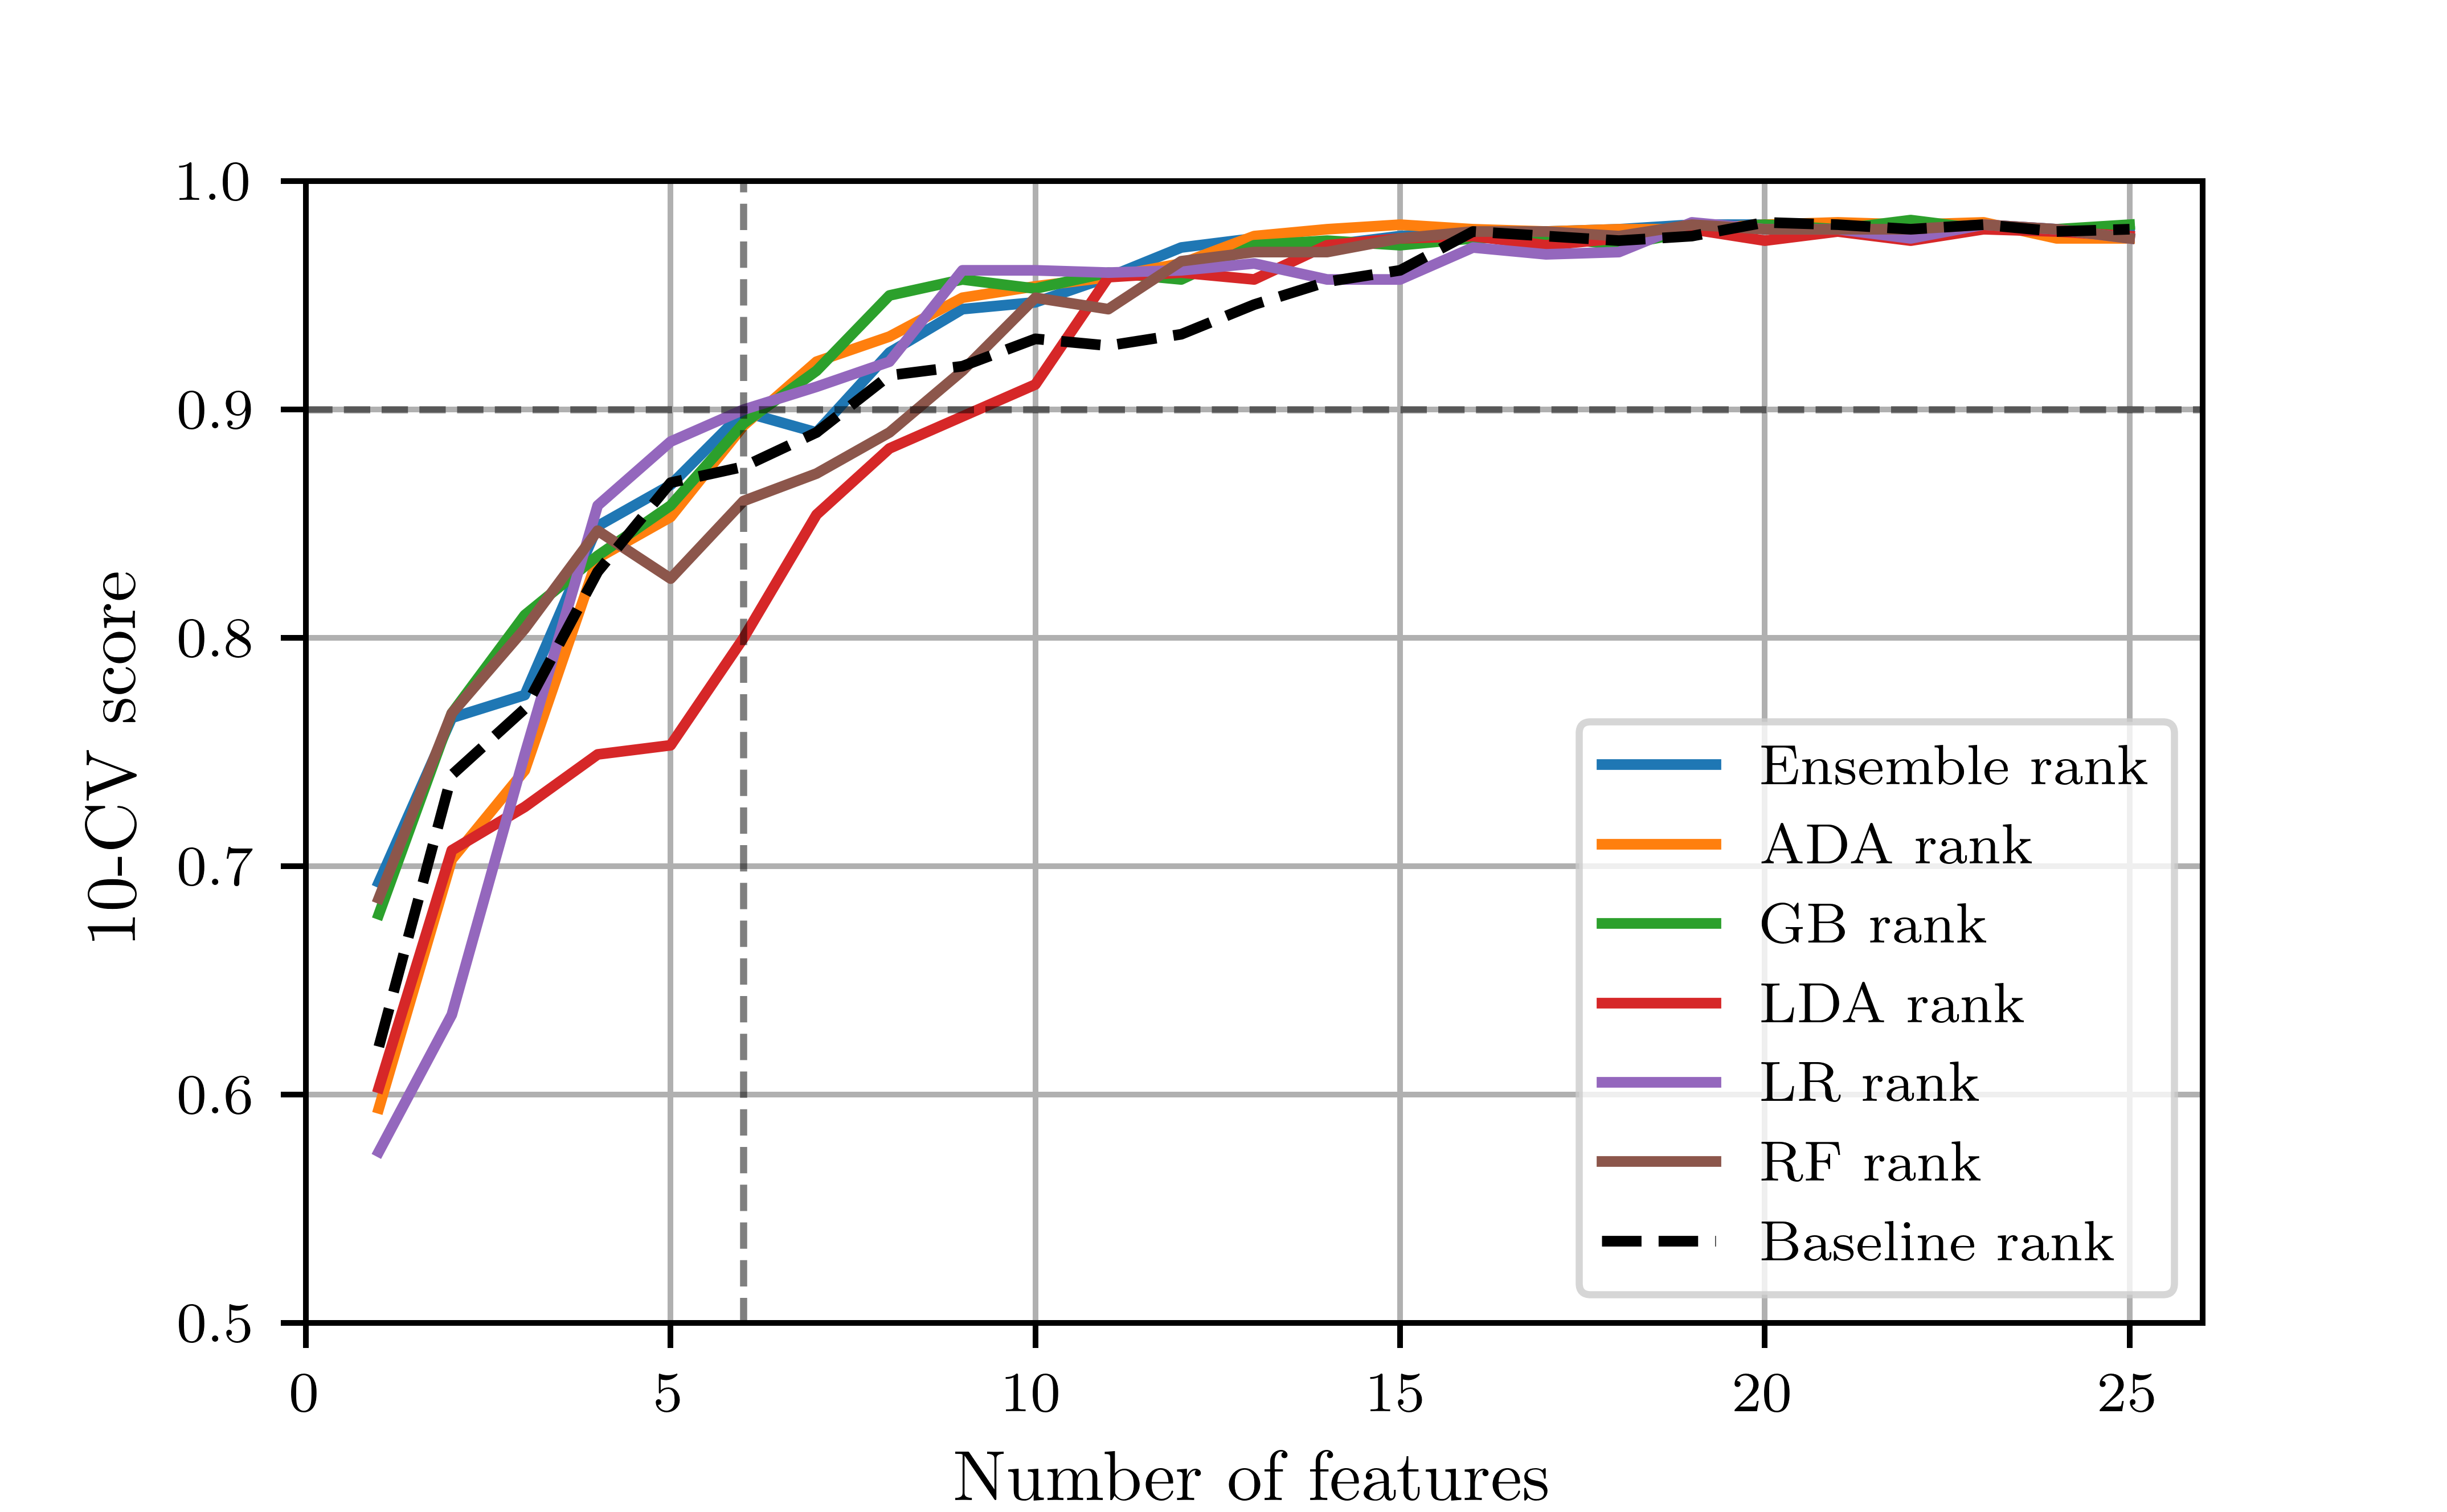
\includegraphics[width=\textwidth]{figures/cv_svm_allrank.png}
        % \caption{SVM}
        % \label{fig:t-SNE_1}
    \end{subfigure}
    \hfill
    \begin{subfigure}[b]{0.49\textwidth}
        \centering
        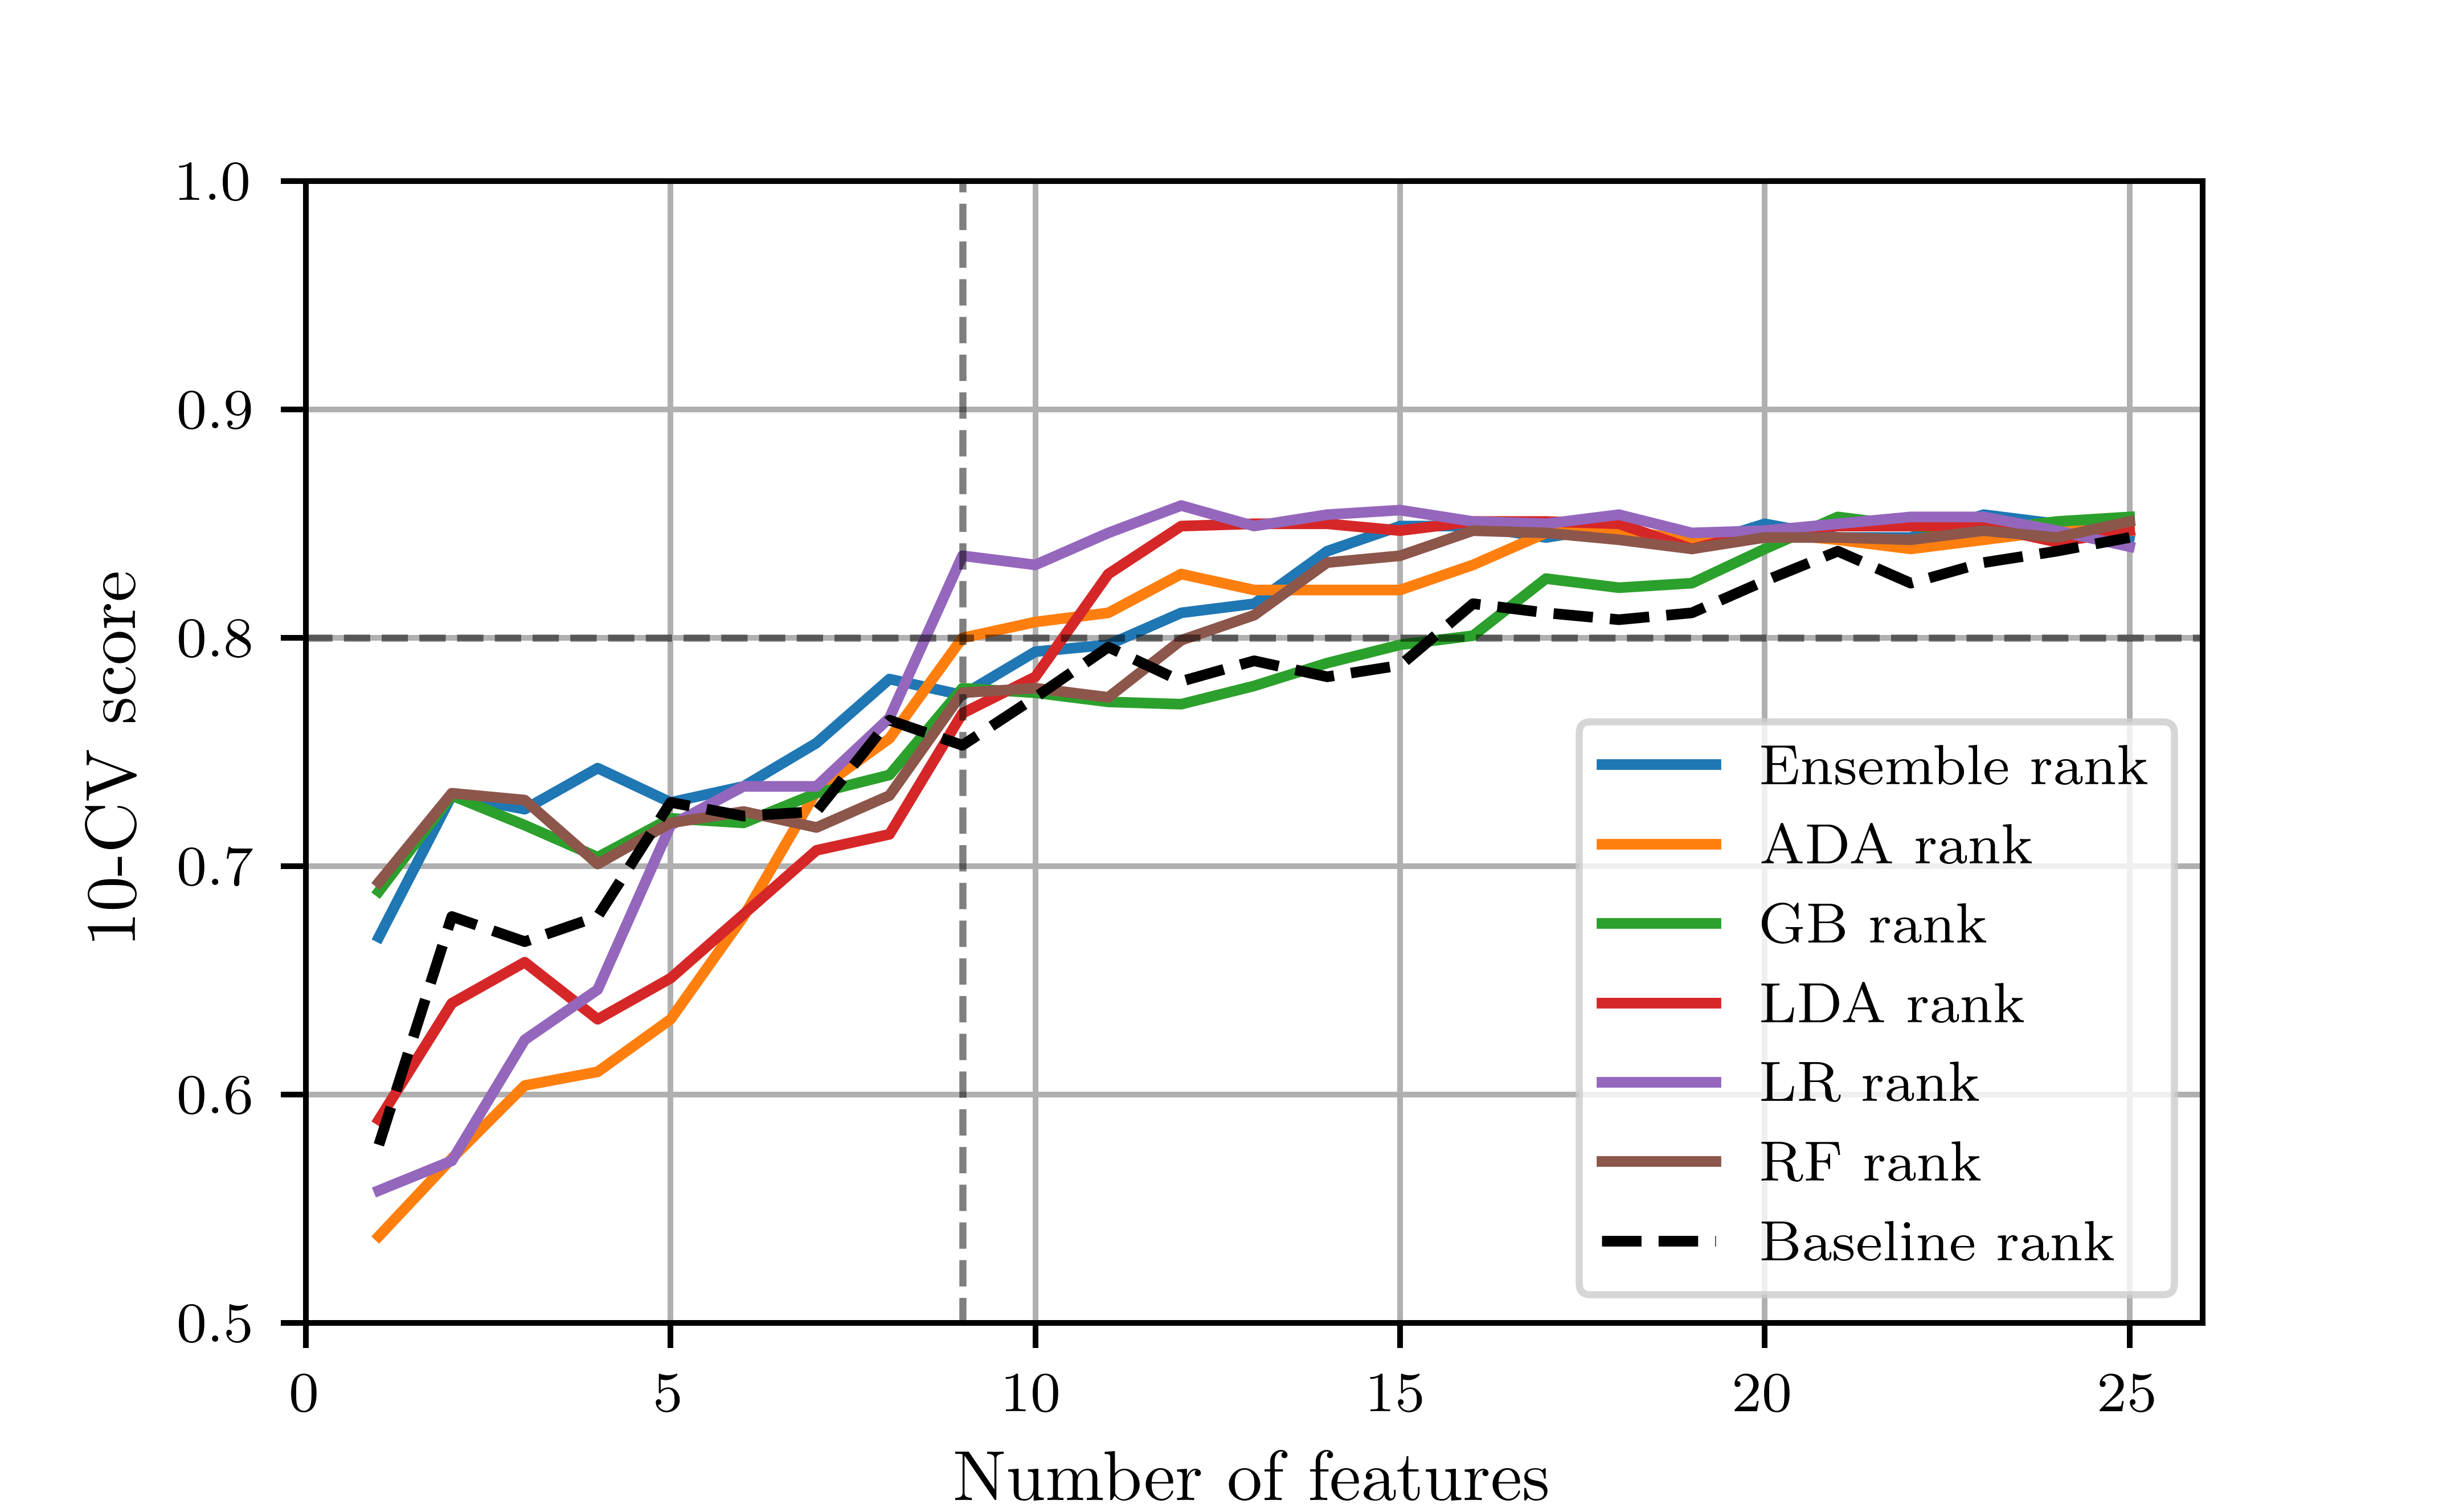
\includegraphics[width=\textwidth]{figures/cv_lr_allrank.png}
        % \caption{LR}
    \end{subfigure}
    \\
    \centering
    \begin{subfigure}[b]{0.49\textwidth}
        \centering
        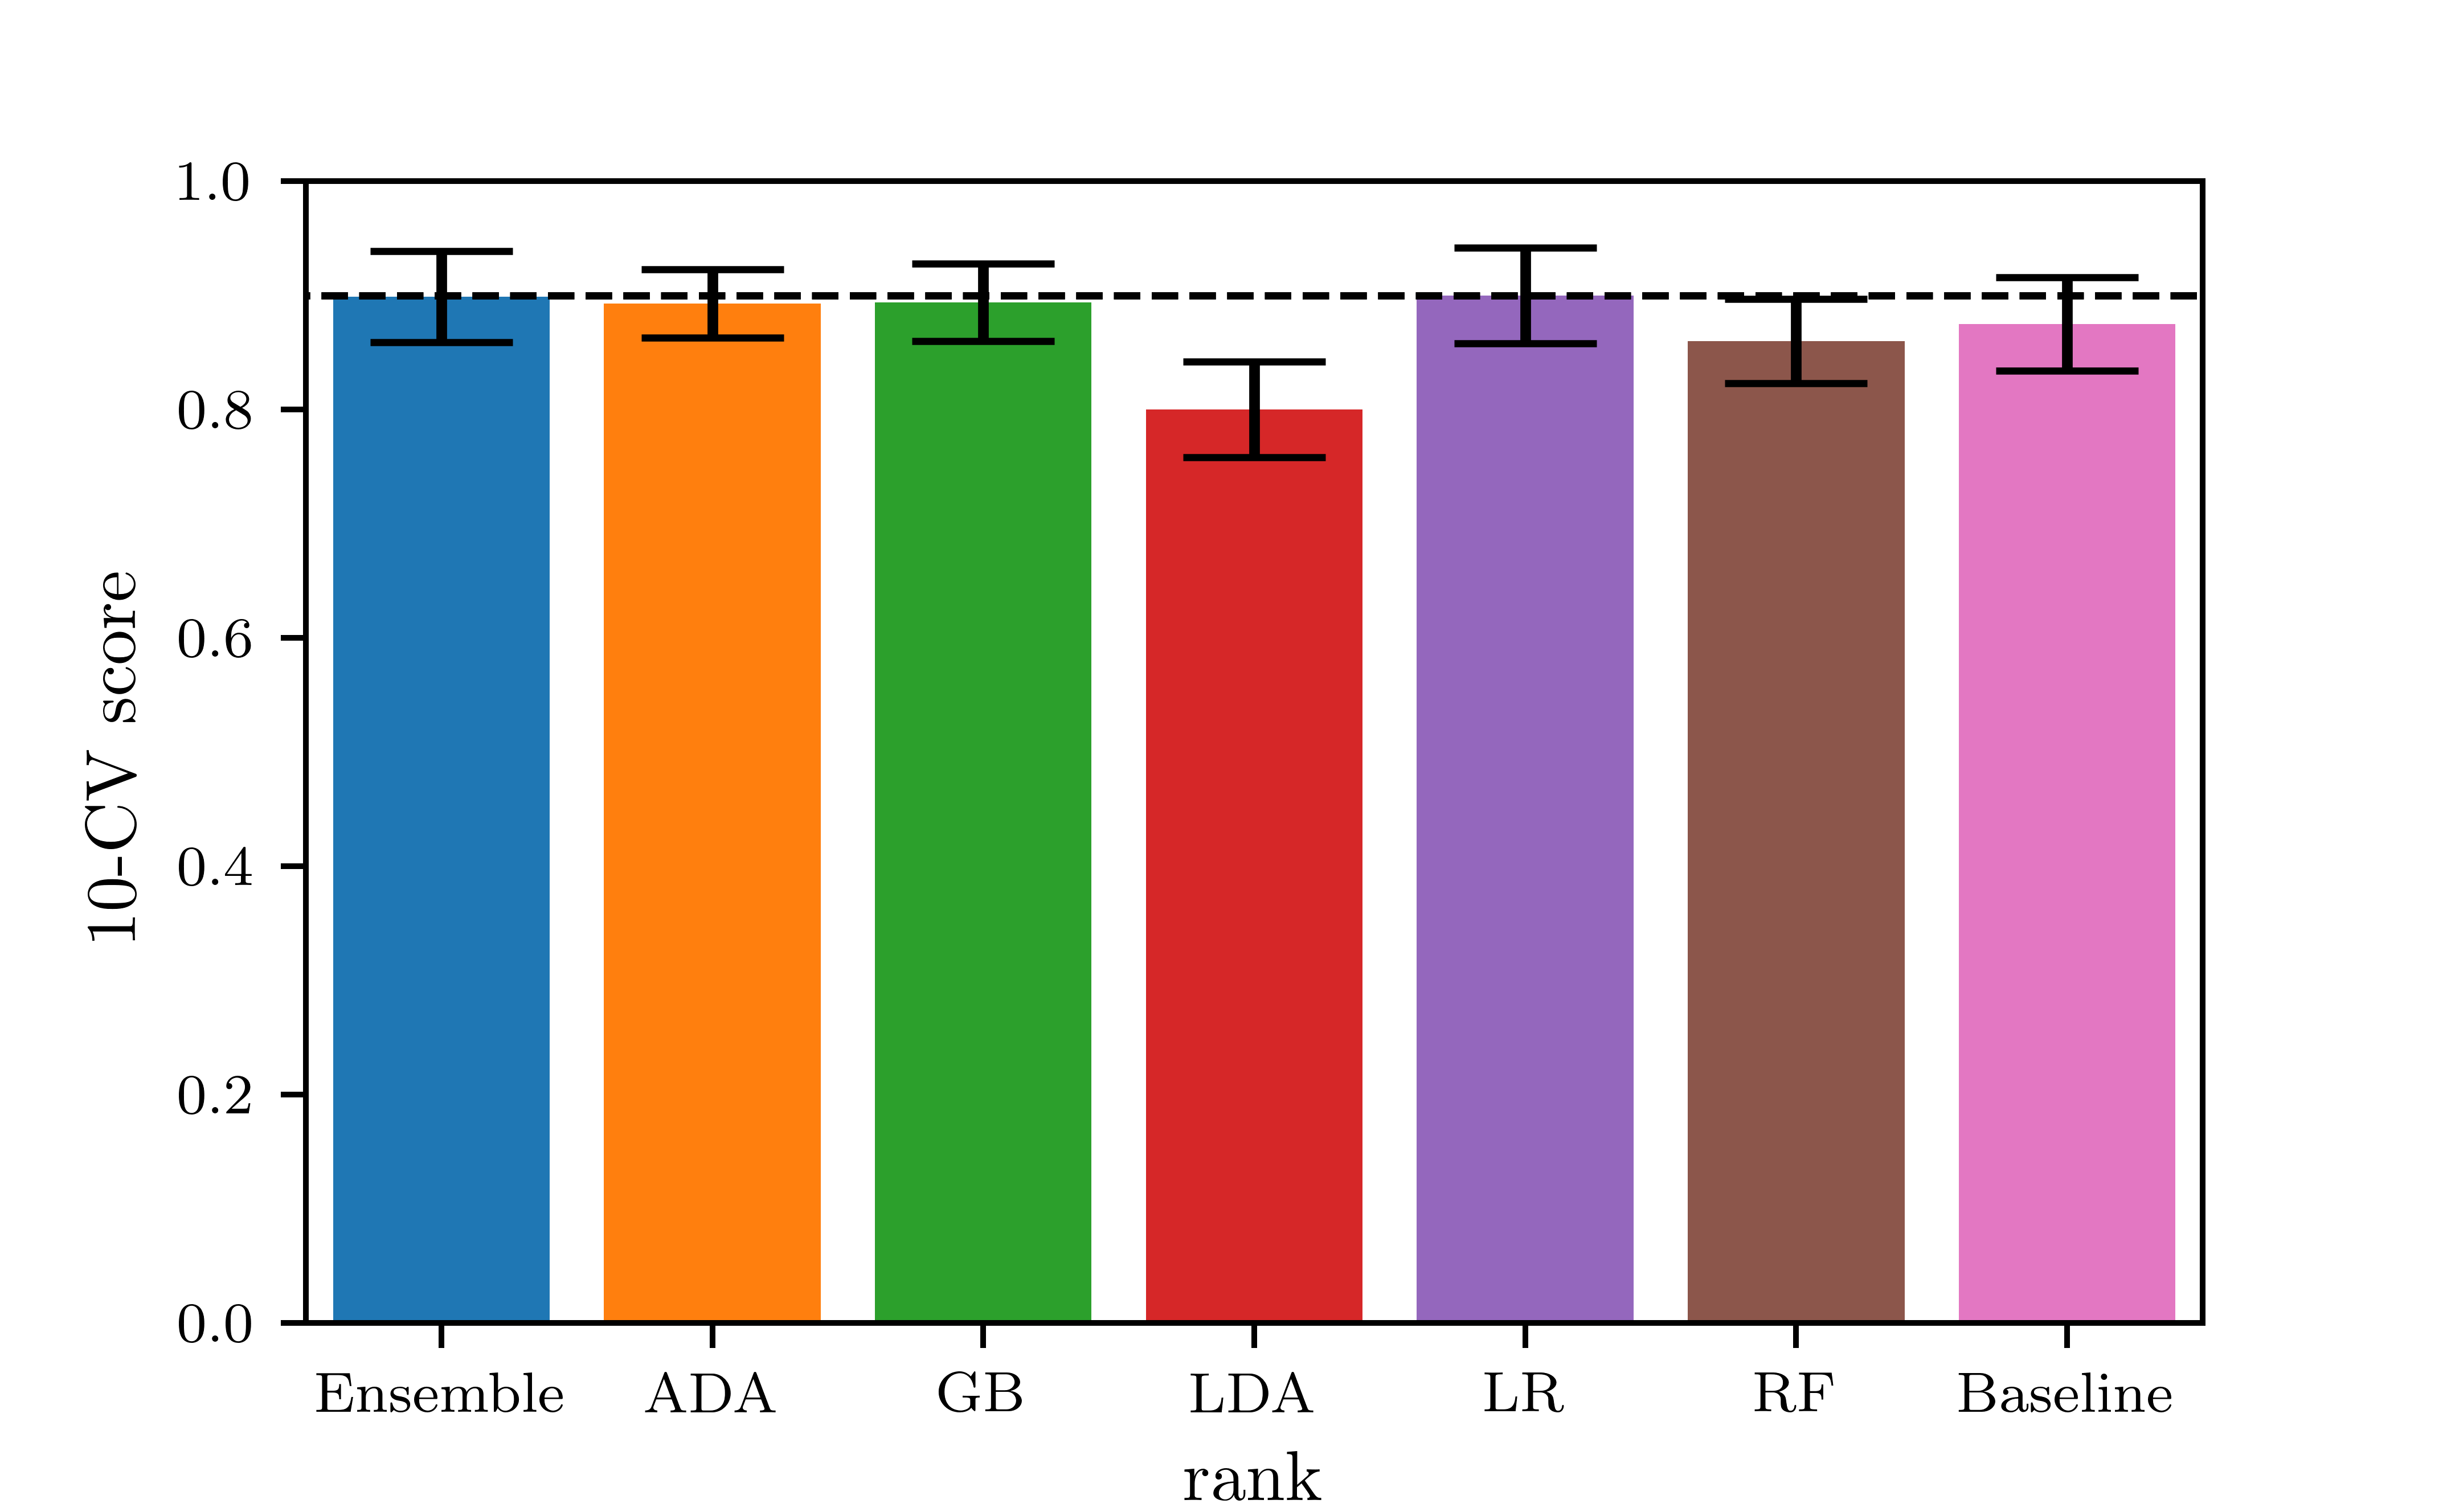
\includegraphics[width=\textwidth]{figures/bar_svm_at_6.png}
        \caption{SVM}
        \label{fig:cv_svm}
    \end{subfigure}
    \hfill
    \begin{subfigure}[b]{0.49\textwidth}
        \centering
        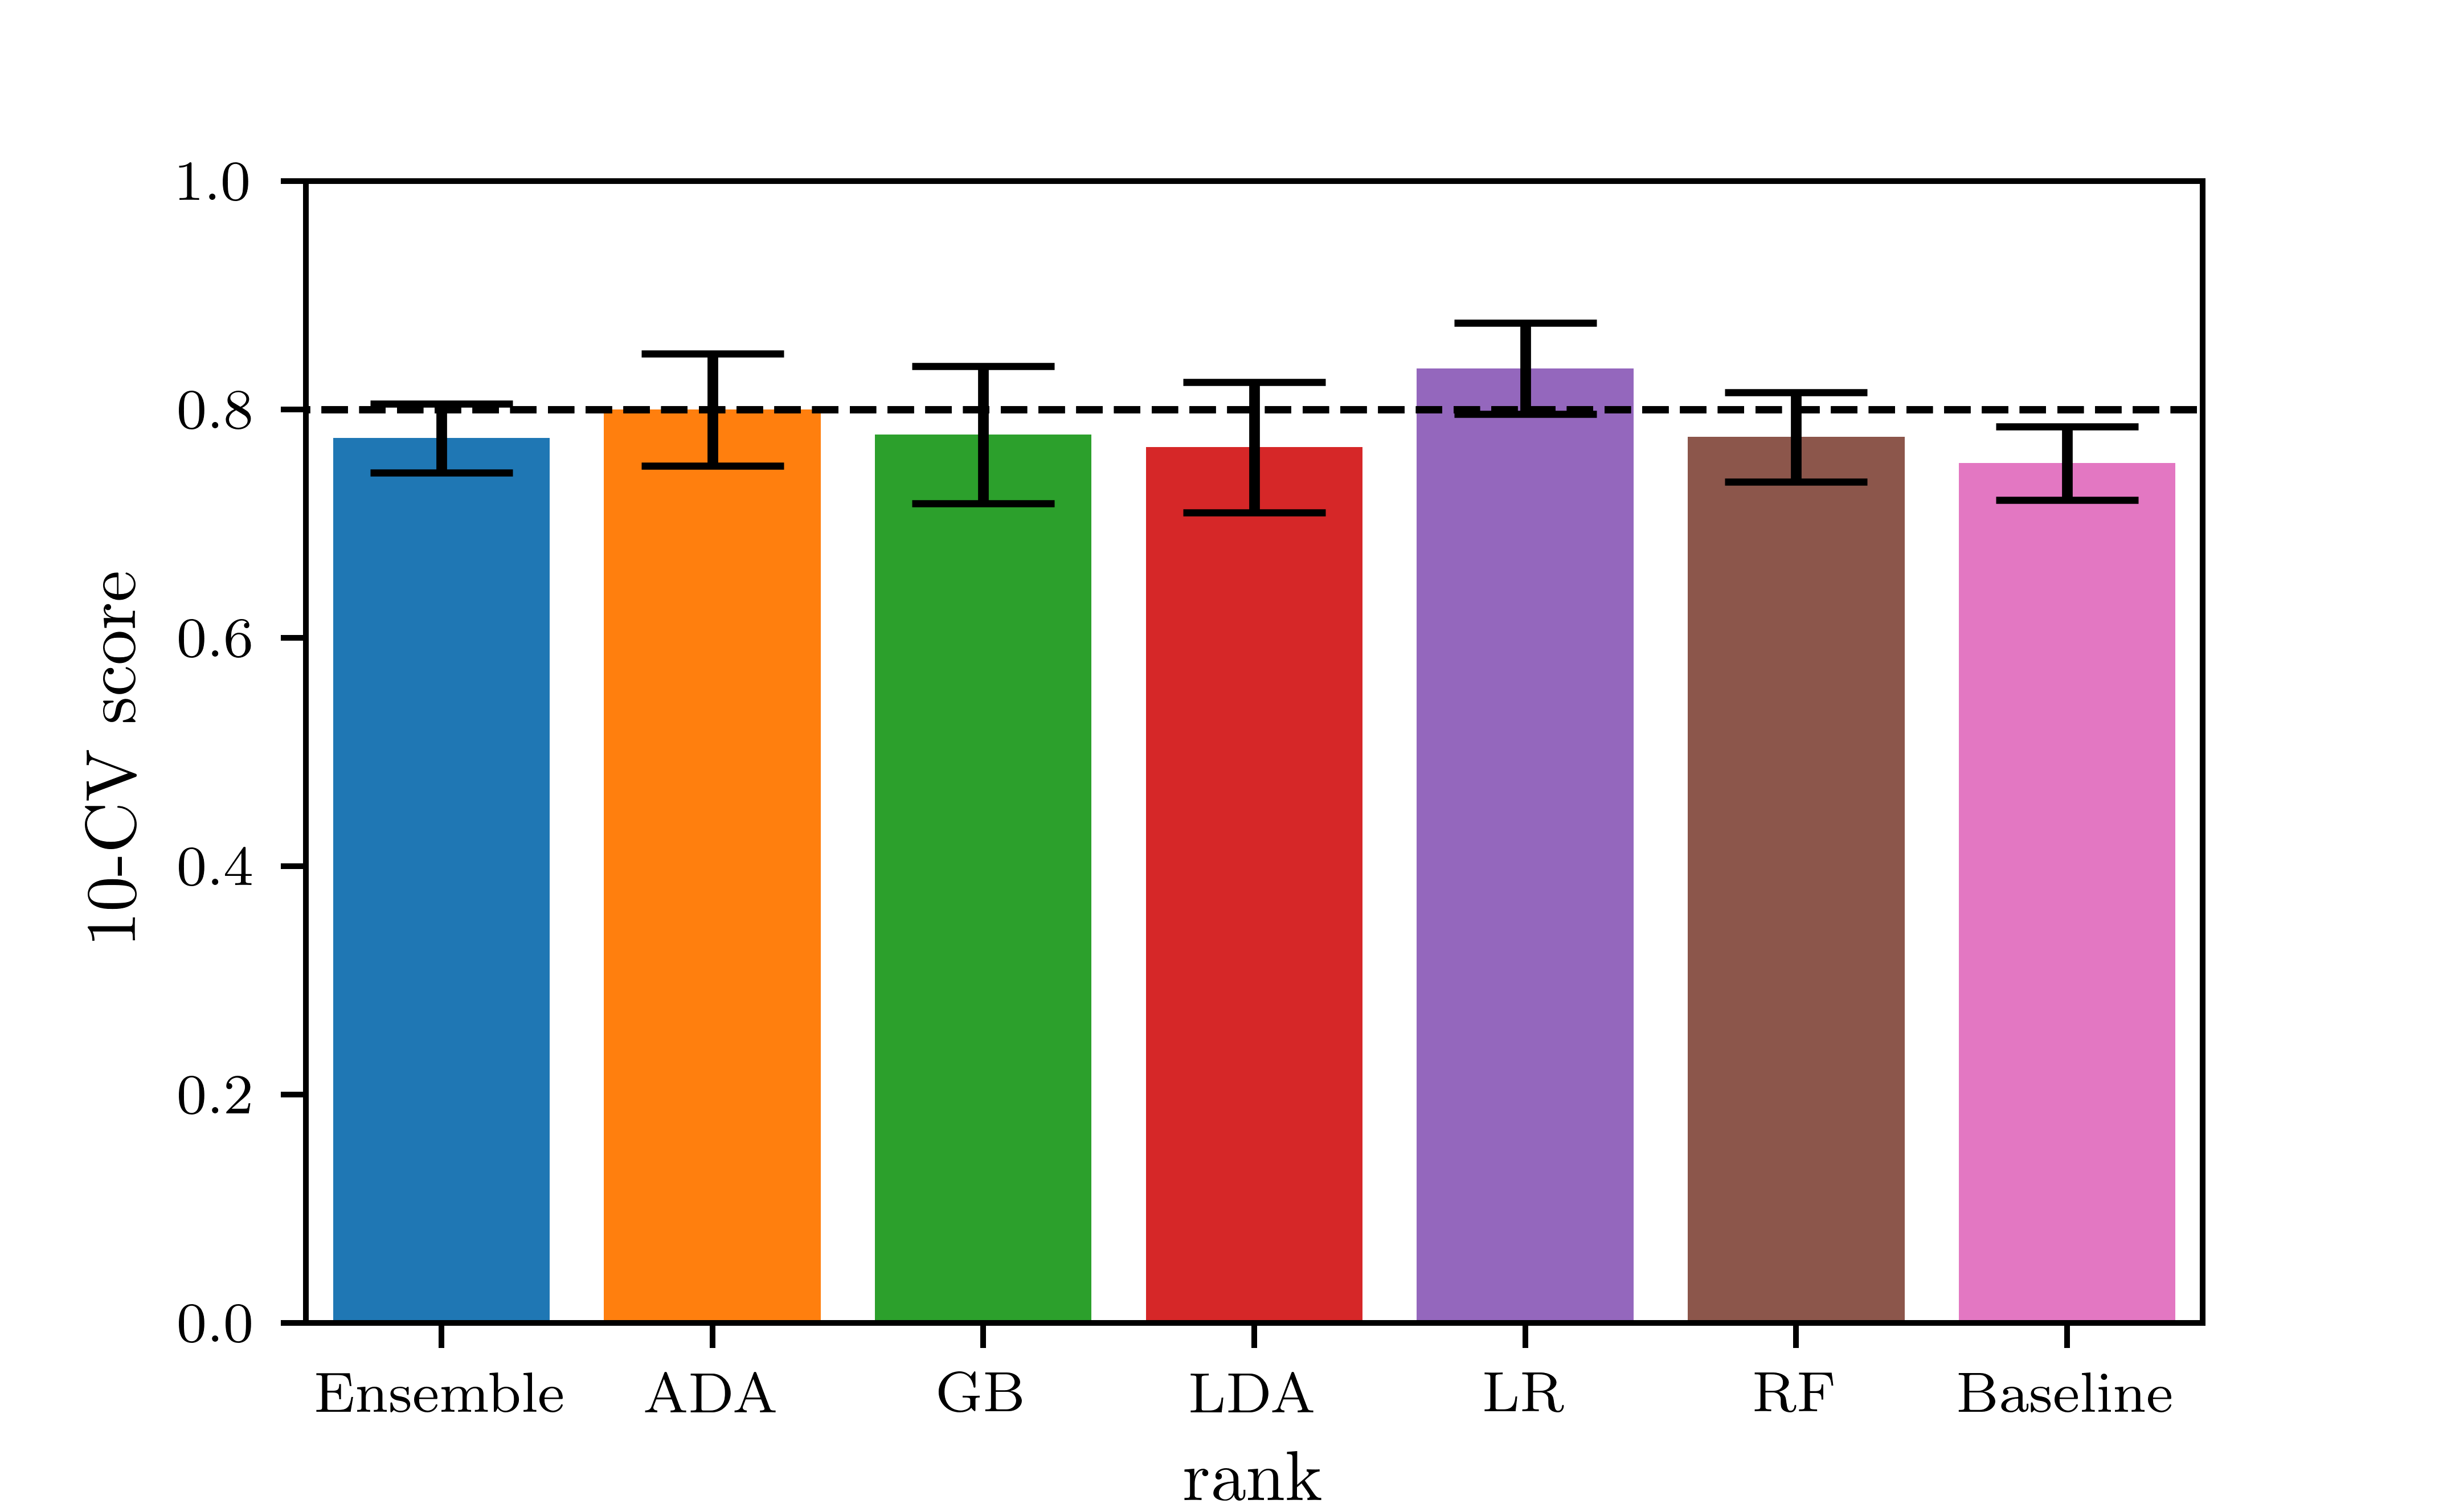
\includegraphics[width=\textwidth]{figures/bar_lr_at_9.png}
        \caption{LR}
    \end{subfigure}
\end{figure}

We found that a final SVM with the Radial Basis Function (RBF) kernel achieves a 0.9 10-CV score when using the top six features from $\text{Rank}_{\text{LR}}$ and $\text{Rank}_{\text{Ensemble}}$, as shown in Figure~\ref{fig:cv_svm}. The top eight features in $\text{Rank}_{\text{Ensemble}}$ are $\text{beta}_{f}$, $\text{F3}_{\text{delta}}$, $\text{F4}_{\text{delta}}$, $\text{F3}_{\text{beta}}$, $\text{P4}_{\text{delta}}$, $\text{F3}_{\text{gamma}}$, $\text{P4}_{\text{theta}}$, and $\text{C3}_{\text{theta}}$. In addition, t-SNE seems to suggest that the top six $\text{Rank}_{\text{Ensemble}}$ features better reflect the stress grouping than a baseline ranking obtained from the earlier simple individual t-tests, as shown in Figure~\ref{fig:t-SNE_baseline-ensemble}.

\begin{figure}[h!]
    \caption{2D embeddings by t-SNE of the top six features selected by $\text{Rank}_{\text{Baseline}}$ and $\text{Rank}_{\text{Ensemble}}$. Green and red samples indicate less stressed and more stressed groups, respectively, and point shape indicates correct(`.') or incorrect(`x') classification results with a RBF-SVM. The $\text{Rank}_{\text{Ensemble}}$ features clearly admit a better separated representation than the $\text{Rank}_{\text{Baseline}}$ features.}
    \label{fig:t-SNE_baseline-ensemble}
    
    \centering
    \begin{subfigure}[b]{0.49\textwidth}
        \centering
        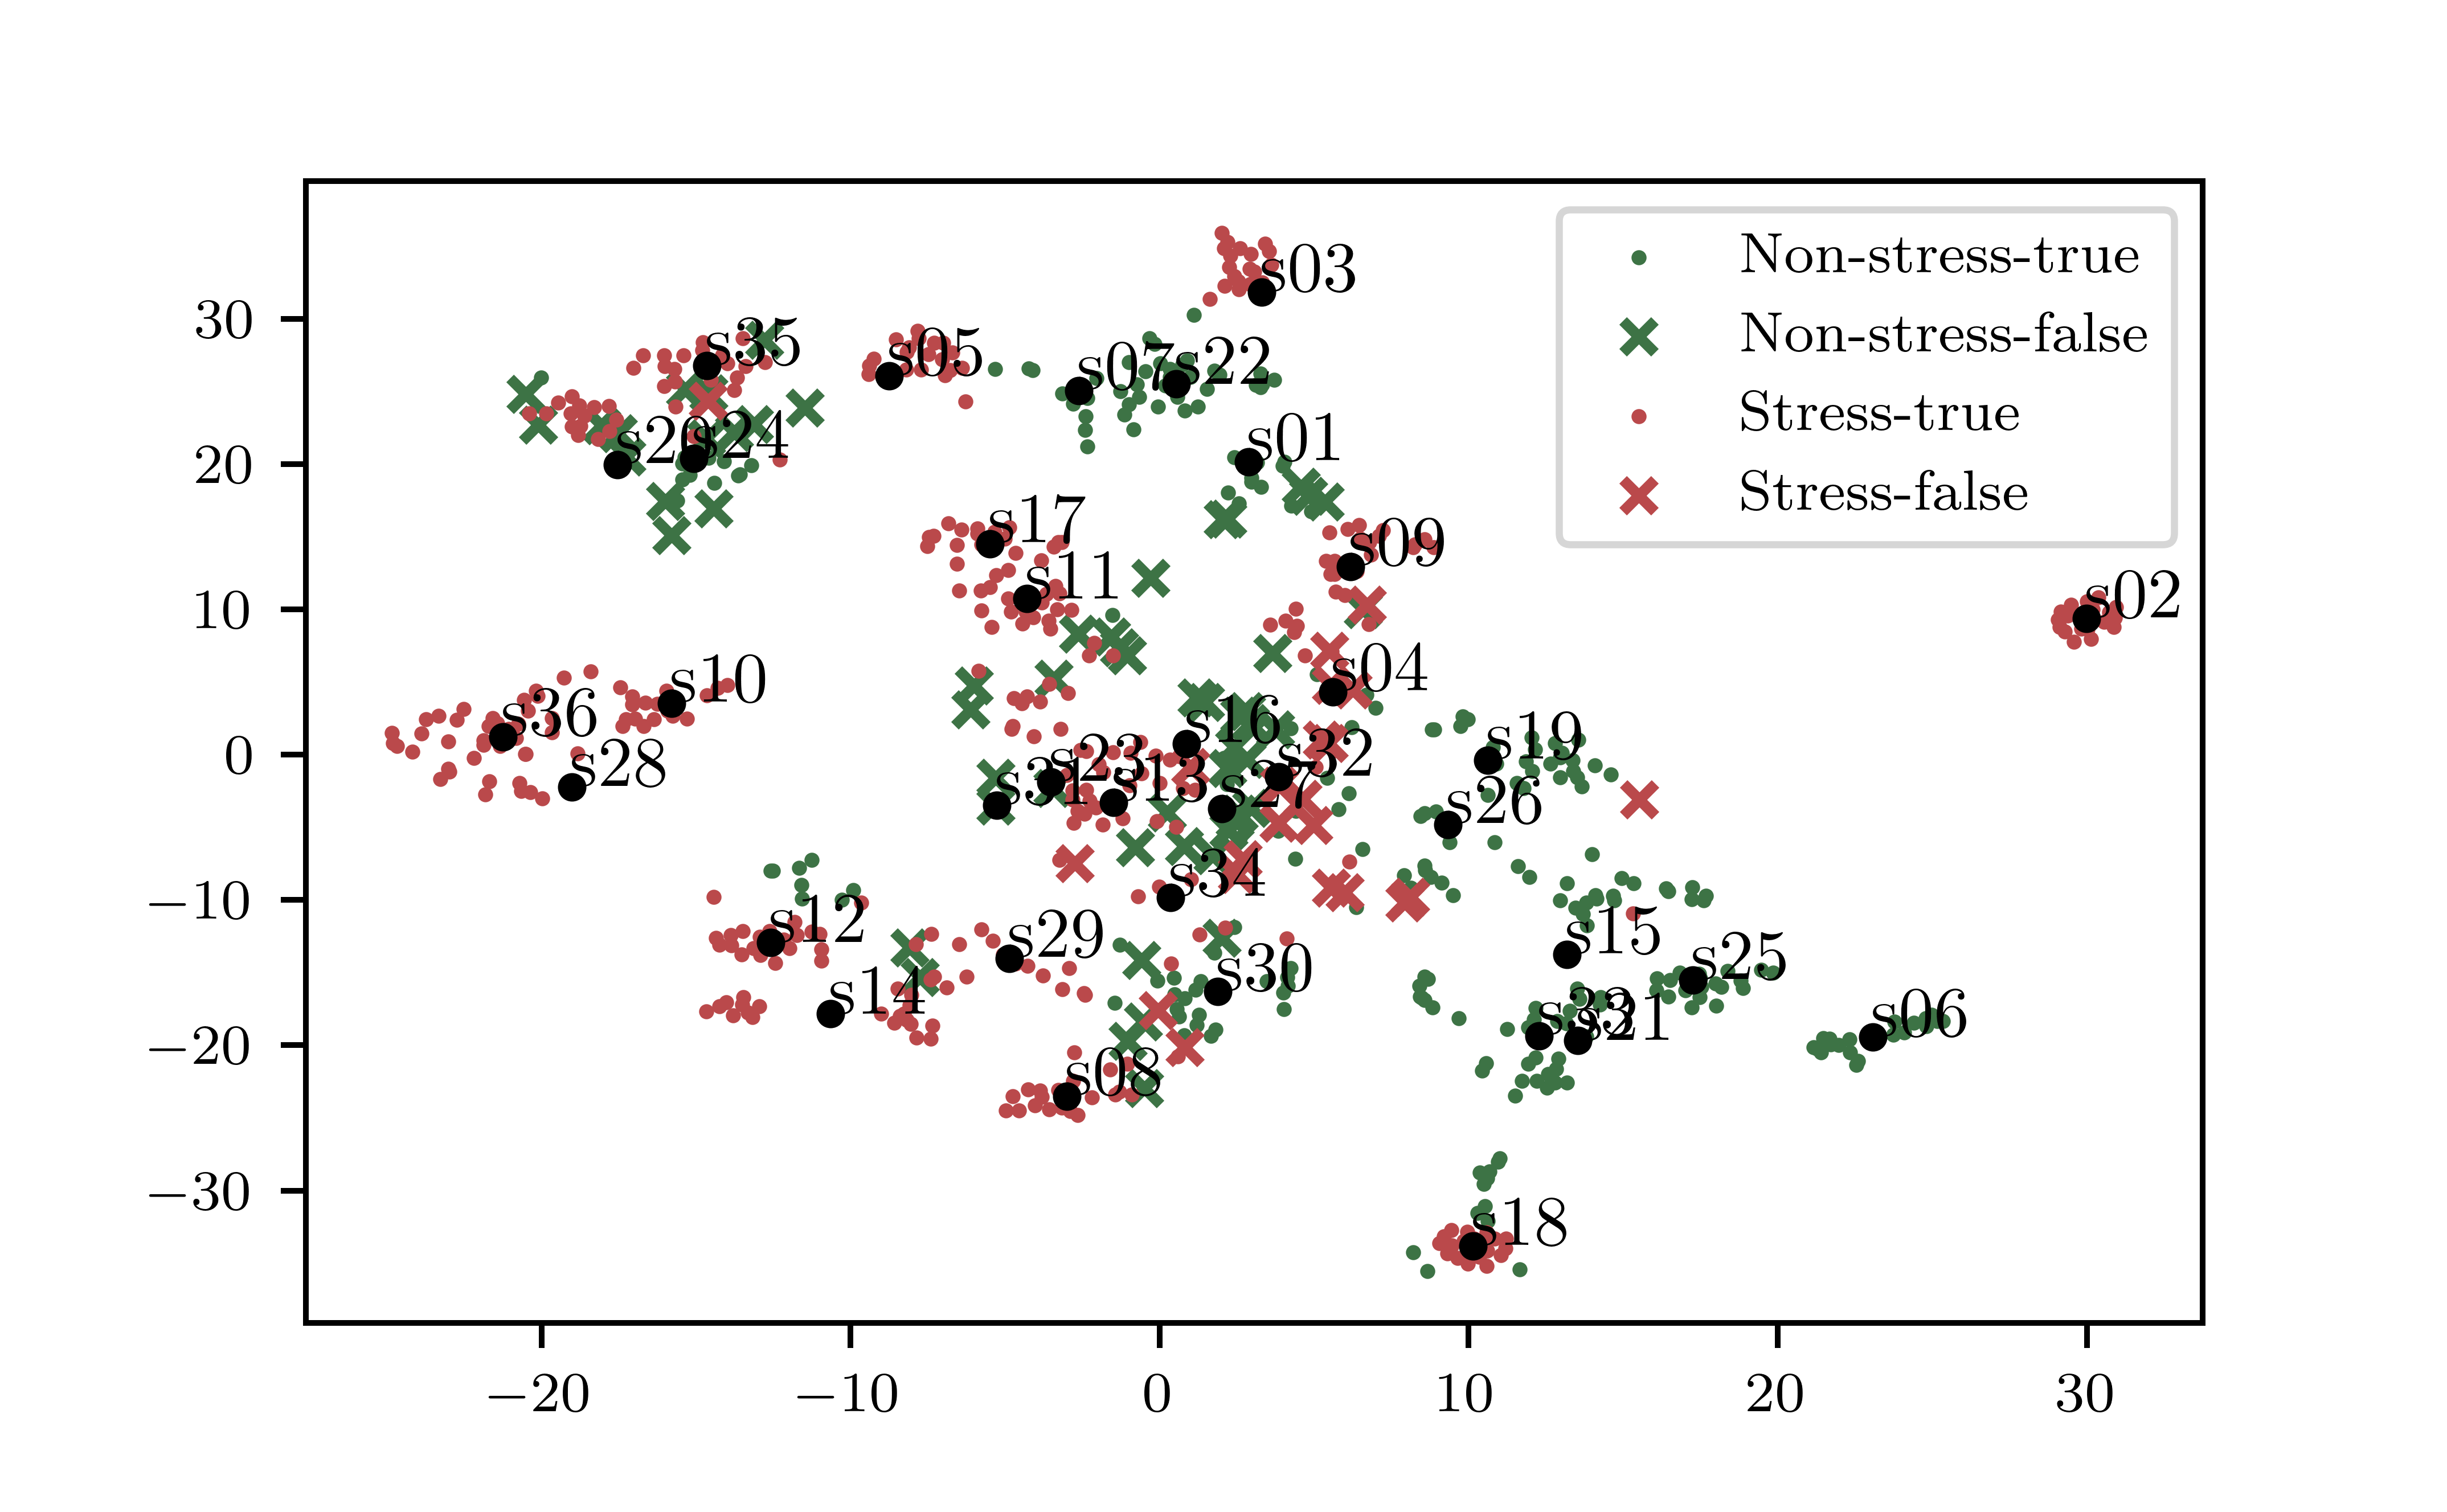
\includegraphics[width=\textwidth]{figures/t-sne-baseline-6.png}
        \caption{Baseline}
        % \label{fig:t-SNE_1}
    \end{subfigure}
    \hfill
    \begin{subfigure}[b]{0.49\textwidth}
        \centering
        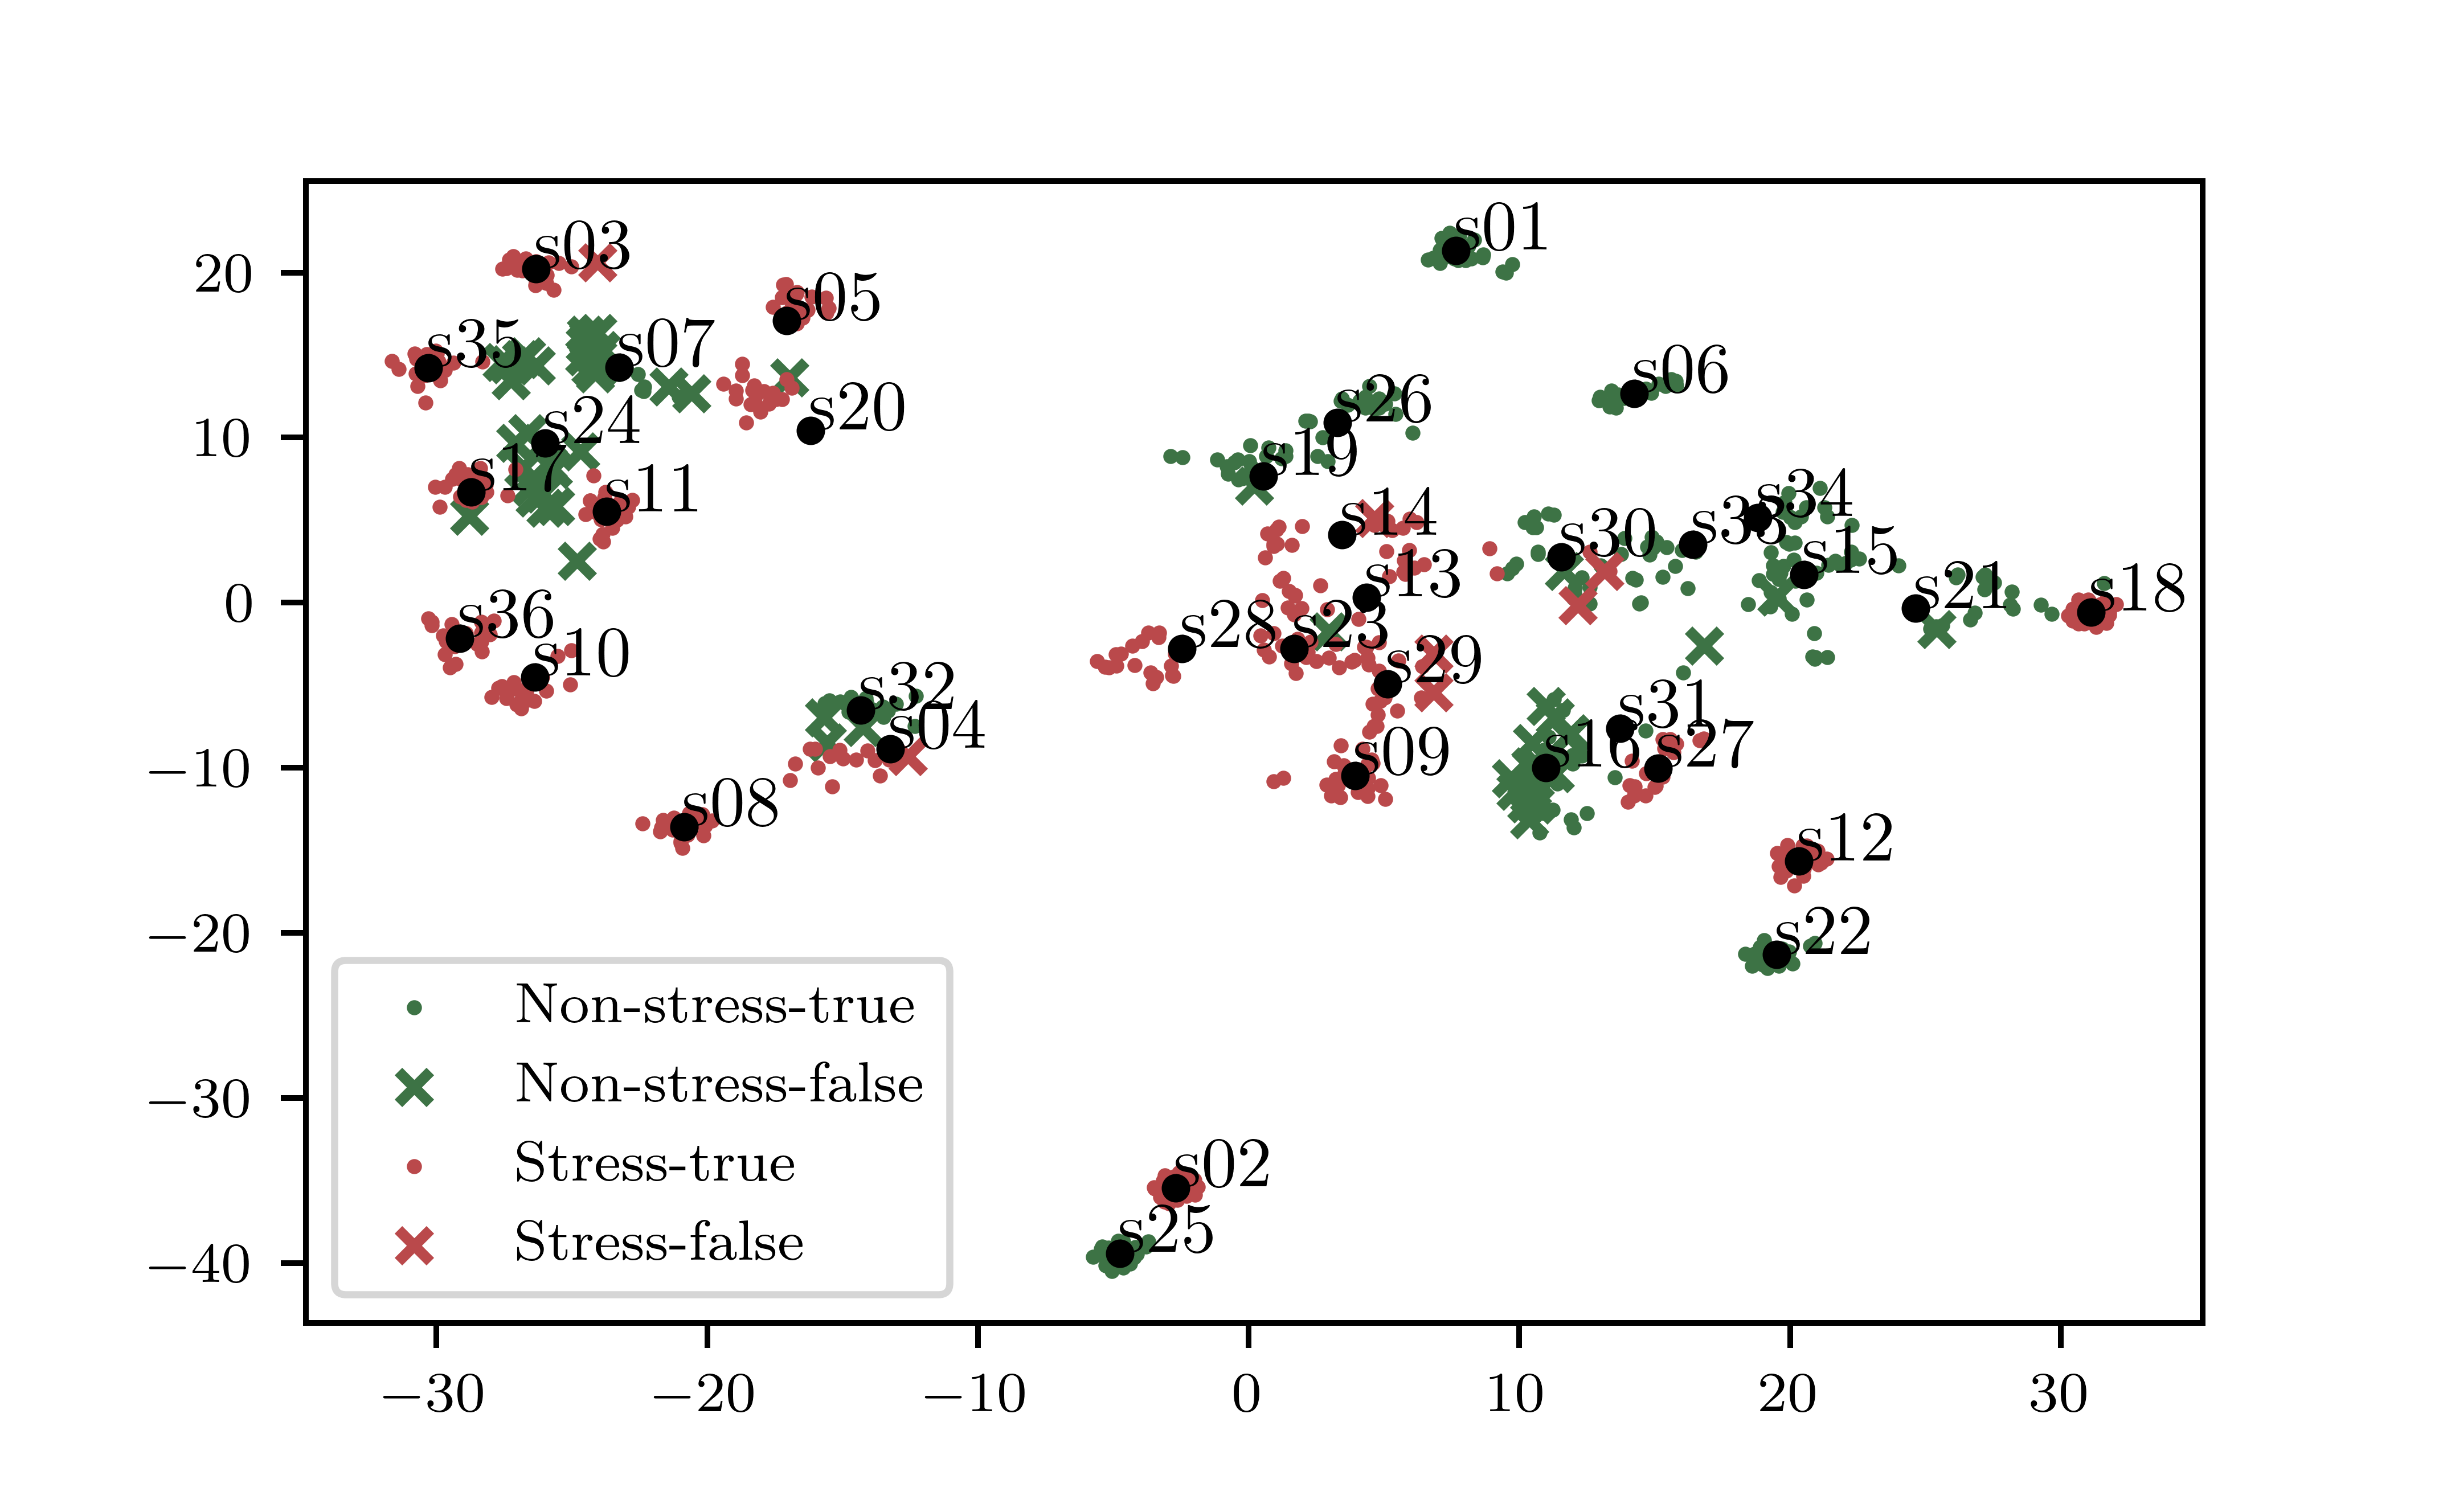
\includegraphics[width=\textwidth]{figures/t-sne-ensemble-6.png}
        \caption{Ensemble}
    \end{subfigure}
\end{figure}

% (5) Significant and contribution

This paper implements and assesses several empirical methods for feature selection that combine a t-test initial selection with feature importance scores based on five different classifiers. Our results confirm that with appropriate feature selection, EEG signals acquired from more stressed and less stressed individuals are sufficiently distinctive to classify them according to stress level, and our top eight features agree with conclusion of previous work finding that the delta and beta frequency bands are the most important frequencies for this task.

\section{Related work} \label{sec2}
Stress is known to cause aberrant reactions in the autonomic nervous system (ANS), including the antagonistic regulation of the sympathetic (SNS) and the parasympathetic (PNS) nervous system \cite{Cohen2000, Hughes2000}. These two systems are associated with stress and relaxation responses, respectively. Changes in the ANS can be detected by EEG signals \cite{Seo2010}. In recent years, EEG signals have emerged as a valid modalist for the analysis of mental states including stress \cite{Awang2011, Hu2015}. EEG signals can be decomposed into frequency bands \cite{Kulkarni2020}, each of which is useful for analysis of different brain states \cite{Alshargie-2018}. A change of power in beta band is associated with alertness, whereas theta band activity occurs throughout the sleep state, and alpha band activity rises with relaxation \cite{Wang2014}. Recent studies have analyzed EEG signals with various signal processing and machine learning methods to detect stress.

Several studies have demonstrated a relationship between stress and EEG signals, and they show that EEG can be used as an input variable for prediction of both short-term and long-term stress. In EEG research, the alpha band is the most commonly used in stress assessment, because it is characterized by increasing activity during relaxation, and decreasing activity during stress \cite{Alshargie-2016}. However, alpha is not the only band that can indicate mental stress. The beta band has also been found to convey signs of mental stress; an increase of power in the beta band is associated with increased alertness when performing cognitive tasks. A relationship between stress and beta band activity at the anterior temporal lobe has been demonstrated when stress-inducing pictures are shown \cite{Seo2010, Awang2011, Hamid2010}. Meanwhile, theta band activity has been used to assess stress during mental arithmetic tasks \cite{Grtner2015}. Moreover, gamma band activity related to slow bands has also been proposed as a biomarker for the identification of stress \cite{Arsalan2019}.

Previous studies have demonstrated the feasibility of using EEG for chronic stress assessment. Chronic stress, unlike acute stress, can be measured without stress-inducing tasks. Since chronic stress is a more related to depressive symptoms than acute stress \cite{McGonagle1990}, and since EEG may be useful as a stress indicator in everyday life \cite{Saeed2020}, we propose the use of EEG signals to identify chronic stress without inducing stress experimentally.

\section{Methodology}\label{sec3}

\subsection{Participants}\label{subsec1}
A total of 55 healthy participants (30 male, 25 female) with ages ranging from 21 to 45 years $(\text{Mean} = 26, SD = 4.84)$ participated in the study. The participants were informed to avoid food and drink with caffeine as well as conditioners, hair creams, sprays, or styling gels on the day of the experiment. Prior to the experiment, all participants gave consent in writing before completing the questionnaire and having their EEG recorded.

\subsection{Data Acquisition}\label{subsec2}
The EEG acquisition phase of the experiment was conducted in a room with a controlled environment. An EEG electrode cap kit was used to record EEG signals of the participants at 125 Hz at 16 active points, namely $\text{FP1}$, $\text{FP2}$, $\text{F3}$, $\text{F4}$, $\text{F7}$, $\text{F8}$, $\text{C3}$, $\text{C4}$, $\text{T3}$, $\text{T4}$, $\text{T5}$, $\text{T6}$, $\text{P3}$, $\text{P4}$, $\text{O1}$, and $\text{O2}$, with two reference electrodes according to the electrode locations of the international 10 - 20 system for EEG (Figure~\ref{fig:activeelectrode}). The experimental procedure is shown in Figure~\ref{fig:procedure}. All participants were initially instructed regarding the experimental procedure, signed the consent form, then took the PSS questionnaire. Each participant was placed comfortably in a chair and asked to close their eyes for 10 minutes while keeping their head motionless to eliminate movement artifacts. The closed-eyes condition was utilized to simplify data processing (obviating the need to remove blink artifact). This design is consistently with previous research that has found that chronic stress can be predicted from EEG without stress induction \cite{Khosrowabadi-2011, Peng-2012, Saeed2020}.

In the study, the PSS-10 questionnaire was used to assess and classify participants' stress levels. The questionnaire has 10 questions, each of which asks about the frequency of stress the subject has experienced in the last month. Each question is answered on a scale of 0 (the incident never happened), to 4 (it occurs frequently). The group of participants was partitioned into three groups based on their PSS scores, as either stressed, non-stressed, or neutral [TODO]. PSS thresholds were chosen as

\begin{equation} \label{eq:1}
   T_{u} =\mu + \frac{\sigma}{2}
\end{equation}

\begin{equation} \label{eq:2}
   T_{l} =\mu - \frac{\sigma}{2},
\end{equation}

where $\mu$ is the mean and $\sigma$ is the standard deviation of the full group's PSS scores over all 55 participants, $T_{u}$ is the upper threshold, and $T_{l}$ is the lower threshold. Any participants with PSS score lower than $T_{l}$ were labeled as non-stressed, and those with PSS scores higher than $T_{u}$ were labeled as stressed. Participants in the intermediary range were labeled as neutral and not used in the feature selection or classification experiment.

\begin{figure}[h!]
  \centering
  \caption{Experimental procedure and data acquisition process}
  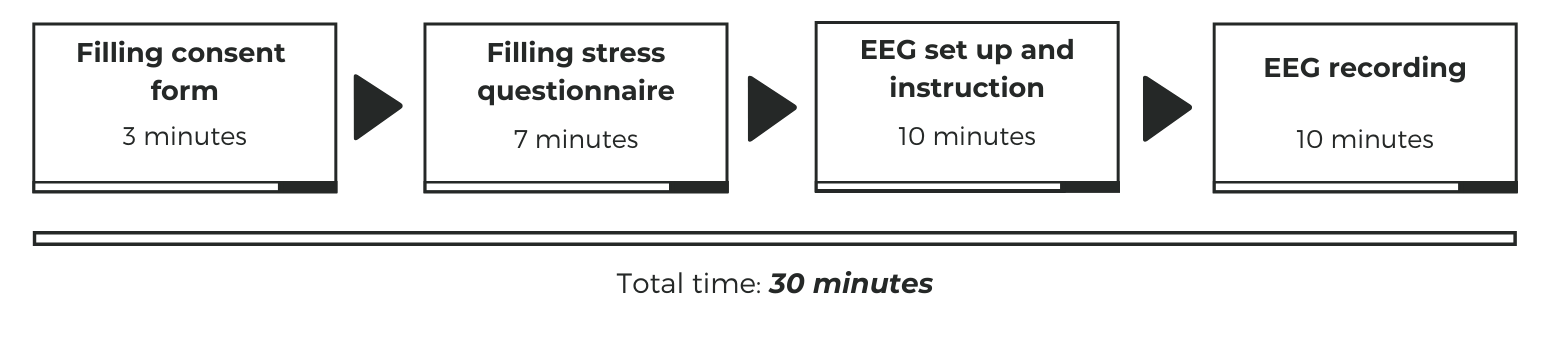
\includegraphics[width=1\textwidth]{Experimentalprocedure.png}
  \label{fig:procedure}
\end{figure}

\begin{figure}[h!]
 \centering
  \caption{Electrode locations of International 10-20 system for EEG recording \cite{wiki:10-20}.}
  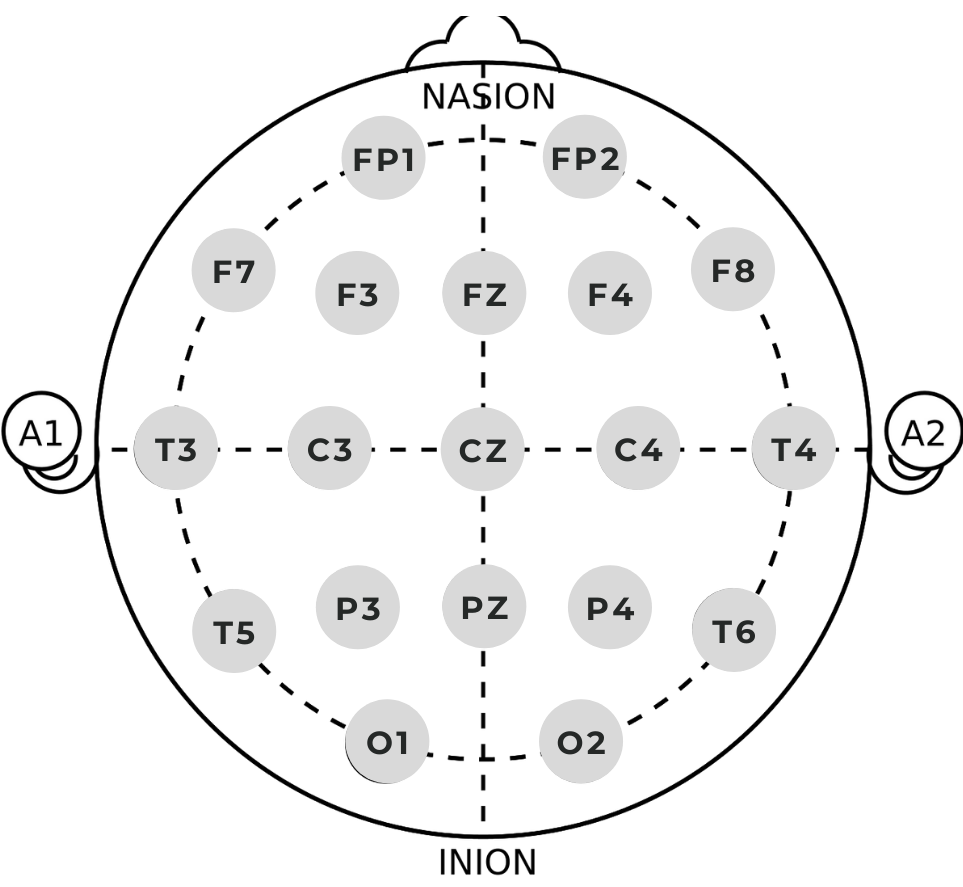
\includegraphics[width=0.5\textwidth]{Electrodeplacement.png}
  \label{fig:activeelectrode}
\end{figure}

\subsection{Feature Extraction}\label{method:featureExtraction}

The first five minutes of the participants' rest-state EEG signals were segmented into 20 smaller records (15 seconds each). For each record, the five EEG frequency bands were obtained using the \texttt{psd\_welch} function from in the \texttt{mne} library. The function calculates power spectral density (PSD) of multiple smaller windows and average them to get a smoother result. The frequency bands, namely, delta (1-3 Hz), theta (4-7 Hz), alpha (8-12 Hz), beta (13-30 Hz), gamma (25-43 Hz), slow (4-13 Hz), and $\text{beta}_{\text{low}}$ (13-17 Hz) were computed from each electrode. We did not perform any other preprocessing. The ratio of gamma to slow bands was used to calculate the $\text{gamma}_{\text{relative}}$ feature. Moreover, there were five alpha and beta asymmetries. The following formulae were used to compute the alpha asymmetries:

\begin{equation} \label{eq:3}
   \alpha_{f} =\frac{ \text{F4}_{\alpha} - \text{F3}_{\alpha} }{ \text{F4}_{\alpha} + \text{F3}_{\alpha} }
\end{equation}

\begin{equation} \label{eq:4}
    \alpha_{t} =\frac{ \text{T4}_{\alpha} - \text{T3}_{\alpha} }{ \text{T4}_{\alpha} + \text{T3}_{\alpha} }
\end{equation}

\begin{equation} \label{eq:5}
   \alpha_{a} ={\alpha_{f}+\alpha_{t}}
\end{equation}

$\alpha_{f}$, $\alpha_{t}$ and $\alpha_{a}$ indicate frontal, temporal, and alpha asymmetries, respectively, and $\text{channel}_\alpha$ denotes the PSD of alpha at each electrode. The beta asymmetry was computed over the frontal and temporal region using the same procedure:

\begin{equation} \label{eq:6}
    \beta_{f} =\frac{ \text{F4}_{\beta} - \text{F3}_{\beta} }{ \text{F4}_{\beta} + \text{F3}_{\beta} }
\end{equation}

\begin{equation} \label{eq:7}
    \beta_{t} =\frac{ \text{T4}_{\beta} - \text{T3}_{\beta} }{ \text{T4}_{\beta} + \text{T3}_{\beta} }
\end{equation}

$\beta_{f}$ and $\beta_{t}$ indicate frontal and temporal asymmetries of the beta band, and $\text{channel}_\beta$ denotes the PSD of beta at each electrode.

In total, we extracted $(16 \times 8) + 5 = 133$ features.

\subsection{Feature Selection}\label{sec:feature_selection}
% We segmented data into 15ssecond segments (20 samples from each participant) followed by the feature extraction process. 

We normalized each of the 133 features across the entire dataset using z-scaling:

\begin{equation} \label{eq:normalized}
   \mathbf{X}^{\prime}_i = \frac{\mathbf{X}_i - \mu_i}{\sigma_i},
\end{equation}

where $\mu_i$ is the mean and $\sigma_i$ is the standard deviation of the data for feature $i$ over all samples across the entire dataset.

Next, we eliminated features unlikely to be useful for classification by comparing the conditional means of each feature over each class (more stressed and less stressed) separately using t-tests for the null hypothesis of equal means. From the original 133 features, we found that 25 of t-tests gave $p < .001$, so we retained these 25 features for further consideration.

We then ranked the 25 features using seven methods:

\begin{enumerate}
    \item $\text{Rank}_{\text{Baseline}}$: <Will investigate t-value>.
    \item $\text{Rank}_{\text{LR}}$: ranked according to the absolute value of the logistic regression coefficient assigned to the feature.
    \item $\text{Rank}_{\text{LDA}}$: ranked according to the absolute value of the linear discriminant analysis coefficient assigned to the feature.
    \item $\text{Rank}_{\text{AB}}$: ranked according to the feature importance score given by AdaBoost. The importance score is the sum of the weight of each weak classifier utilizing the feature in question. [TODO: Recheck]
    \item $\text{Rank}_{\text{GB}}$: ranked according to the feature importance score given by gradient boosting. The importance score is the sum of the weight of each weak classifier utilizing the feature in question. [TODO: Recheck]
    \item $\text{Rank}_{\text{RF}}$: ranked according to the feature importance score given by random forest. The importance score is the sum of the weight of each weak classifier utilizing the feature in question. [TODO: Recheck]
    \item $\text{Rank}_{\text{Ensemble}}$: ranked according to a score based on the previous five rankings. The score for feature $i$ is
\end{enumerate}

\begin{equation} \label{eq:rank_score}
   \text{score}_i = \sum_{m\in M} \text{Rank}_{m}[i],
\end{equation}

where $M = \{\text{LR}, \text{LDA}, \text{AB}, \text{GB}, \text{RF} \}$, and $i$ is the index of the feature of interest. $\text{Rank}_{\text{Ensemble}}$ is obtained by sorting the scores in ascending order. Thus, the feature with the lowest score (summed rank) is the most important one.

\subsection{Classification}\label{subsec4}
We utilize two classifiers commonly used in previous studies \cite{Alshargie-2018, Subhani-2017, Saeed2020, Kotsiantis2007}: logistic regression (LR) and the support vector machine (SVM).

\subsubsection{Logistic Regression (LR)}
In its simplest form, logistic regression is a generalized linear model for the Bernoulli (binary class) distribution that employs a logistic sigmoid in a linear combination of the features to represent a binary dependent variable i.e., $ \text{p} ( \text{y} \vert \text{x} ) $.

\subsubsection{Support Vector Machine (SVM)}
A support vector machine performs linear binary maximum margin classification in a feature space. SVMs have been shown to be very effective in EEG-based stress categorization studies \cite{Alshargie-2018, Subhani-2017}. A linear SVM would give a similar result to LR, but with a nonlinear transformation into feature space, SVMs can give higher accuracy.

[TODO: Add LDA, Ada, RF, Boost]

\subsection{Performance Metrics}\label{subsec5}
A 10-CV score is used to measure the classification performance. t-SNE is used to visualize the similarity between samples. 

\section{Results}\label{sec4}
% The objective of this study was to understand the effectiveness of EEG in chronic stress assessment. The results of this study, which include group labelling, experimental results, feature selection, and classification were interpreted.

\subsection{Groups Labeling} \label{subsec6}
A total of 55 participants can be divided into 3 groups consisting of Stress, Non-Stress, and Neutral groups based on the PSS questionnaire score. From the Equation~\ref{eq:1} and Equation~\ref{eq:2}, we obtain the $\mu$, $\sigma$ = (20.75$\pm$6.13). The score lower than 17.68 is considered to be Non-Stress group, whereas the score higher than 23.81 is considered to be Stress group. The participants with a score in between the first standard deviation are considered to be in Neutral group and are discarded in the classification. As a result, the Stress group comprises 20 participants, while Non-Stress group comprises 16 participants. In total, the number of subjects in classification is $(20 + 16) = 36$ and $(36 \times 20) = 720$ samples after segmentation.

\subsection{t-test result}
The independent sample t-test with $p < .001$ was used to select feature in this study. For the t-test, the degree of freedom was 1 and the null hypothesis was tested for EEG feature of Stress and Non-Stress groups. The result using the p-values for different features are shown in Table~\ref{tab:featureselection1} and Table~\ref{tab:featureselection2}. 

% It is evident that at a confidence level of $< .001$, delta, theta, and alpha from frontal as well as alpha asymmetry are statistically significant feature in stressed and non-stressed groups. The rest of the feature, which are statistically significant are shown in the Table~\ref{tab:featureselection1} and Table~\ref{tab:featureselection2}.

\begin{table}[h!]
\caption{Results for the t-test on various frequency bands.}
\scalebox{0.75}{
\begin{tabular}{ccccccccc}
\hline
\textbf{}                            & \multicolumn{8}{c}{\textbf{Frequency bands}}                                                                                                                                                                      \\
\multicolumn{1}{l}{\textbf{Channel}} & \textbf{Delta ($\delta$)}       & \textbf{Theta ($\theta$)}       & \textbf{Alpha ($\alpha$)}       & \textbf{Beta ($\beta$)}        & \textbf{Gamma ($\gamma$)}       & \textbf{Slow}           & \textbf{Low Beta}    & \textbf{RG} \\ \hline
FP1                                  & \textbf{\textless .001} & 0.744                   & \textbf{0.002}          & 0.899                   & \textbf{0.024}          & 0.203                   & 0.629                   & 0.221                       \\
FP2                                  & \textbf{0.016}          & \textbf{0.010}          & \textbf{0.041}          & \textbf{0.008}          & 0.956                   & 0.682                   & 0.071                   & 0.168                       \\
F3                                   & \textbf{\textless .001} & \textbf{\textless .001} & \textbf{\textless .001} & \textbf{\textless .001} & \textbf{\textless .001} & \textbf{\textless .001} & \textbf{\textless .001} & 0.864                       \\
F4                                   & \textbf{\textless .001} & \textbf{0.001}          & \textbf{\textless .001} & 0.488                   & 0.276                   & \textbf{0.020}          & 0.479                   & \textbf{0.011}              \\
F7                                   & \textbf{0.006}          & 0.550                   & \textbf{\textless .001} & \textbf{0.015}          & 0.616                   & \textbf{0.026}          & 0.474                   & \textbf{0.011}              \\
F8                                   & 0.115                   & 0.211                   & 0.088                   & \textbf{0.045}          & 0.251                   & 0.789                   & 0.117                   & 0.677                       \\
C3                                   & \textbf{\textless .001} & \textbf{\textless .001} & 0.297                   & 0.069                   & \textbf{0.007}          & \textbf{0.026}          & \textbf{0.003}          & \textbf{\textless .001}     \\
C4                                   & 0.551                   & 0.329                   & 0.316                   & 0.895                   & \textbf{0.016}          & 0.297                   & 0.186                   & 0.146                       \\
T3                                   & 0.090                   & 0.719                   & \textbf{0.001}          & 0.650                   & \textbf{\textless .001} & 0.401                   & 0.608                   & 0.078                       \\
T4                                   & 0.101                   & \textbf{\textless .001} & 0.855                   & \textbf{0.029}          & \textbf{0.003}          & \textbf{0.003}          & \textbf{\textless .001} & \textbf{0.001}              \\
T5                                   & 0.095                   & 0.126                   & 0.213                   & 0.217                   & 0.305                   & 0.482                   & 0.687                   & 0.199                       \\
T6                                   & 0.919                   & 0.840                   & \textbf{\textless .001} & 0.306                   & \textbf{0.003}          & \textbf{0.010}          & \textbf{0.014}          & 0.105                       \\
P3                                   & 0.639                   & 0.507                   & 0.405                   & 0.114                   & 0.068                   & 0.424                   & 0.077                   & 0.358                       \\
P4                                   & \textbf{\textless .001} & \textbf{\textless .001} & \textbf{\textless .001} & 0.573                   & \textbf{0.012}          & 0.630                   & 0.379                   & 0.165                       \\
O1                                   & 0.057                   & 0.169                   & 0.080                   & 0.271                   & 0.128                   & 0.163                   & 0.778                   & 0.469                       \\
O2                                   & \textbf{0.001}          & 0.384                   & 0.388                   & \textbf{0.009}          & 0.544                   & 0.729                   & 0.252                   & \textbf{0.042}              \\ \hline
\end{tabular}} 
    \label{tab:featureselection1}
\end{table}

\begin{table}[h!]
\caption{Results for the t-test on asymmetries}
\scalebox{0.70}{
\begin{tabular}{ccccc}
\hline
\textbf{Alpha asymmetry ($\alpha_{a}$)}   & \textbf{Alpha frontal ($\alpha_{f}$)}   & \textbf{Alpha temporal ($\alpha_{t}$)}   & \textbf{Beta frontal ($\beta_{f}$)}    & \textbf{Beta temporal ($\beta_{f}$)} \\ \hline
\textbf{\textless .001} & \textbf{\textless .001} & \textbf{\textless .001} & \textbf{\textless .001} & \textbf{0.002}       \\ \hline
\end{tabular}}
    \label{tab:featureselection2}
\end{table}

There are 25 features with $p < .001$ which are $\text{FP1}_{\delta}$, $\text{F3}_{\delta}$, $\text{F4}_{\delta}$, $\text{C3}_{\delta}$, $\text{P4}_{\delta}$, $\text{F3}_{\theta}$, $\text{C3}_{\theta}$, $\text{T4}_{\theta}$, $\text{P4}_{\theta}$, $\text{F3}_{\alpha}$, $\text{F4}_{\alpha}$, $\text{F7}_{\alpha}$, $\text{T6}_{\alpha}$, $\text{P4}_{\alpha}$, $\text{F3}_{\beta}$, $\text{F3}_{\gamma}$, $\text{T3}_{\gamma}$, $\text{F3}_\text{slow}$, $\text{F3}_{\text{Low}\beta}$, $\text{T4}_{\text{Low}\beta}$, $\text{C3}_{\text{RG}}$, $\alpha_{f}$, $\alpha_{t}$, $\alpha_{a}$,$\beta_{f}$. We use this as a list for $\text{Rank}_{\text{Baseline}}$.

\subsection{Ranking with coefficient and feature importance score}

We rank the 25 features from the t-test result using coefficient/feature importance score of a classifier as mentioned in the Section~\ref{sec:feature_selection}. To verify any $\text{Rank}_{m}$ where $m \in \{\text{LR}, \text{LDA}, \text{ADA}, \text{GB}, \text{RF}\}$, we (1) iterate over the index of $\text{Rank}_{m}$; (2) select the features from the $\text{Rank}_{m}^{1}$ to $\text{Rank}_{m}^{i}$ where $i$ is the current iteration; (3) calculate the 10-CV score using rbf-SVM and LR; and (4) plot the t-SNE space to visualize the similarity of samples given the features from the iteration that SVM can achieve over $0.9$ 10-CV score.

The 10-CV score threshold of 0.9 for SVM and 0.8 for LR is selected based on the 10-CV score of each model when training the model using 25 features. The SVM exceeds 0.9 10-CV score while LR can reach 0.85 at best. Table that reports every ranks and 10-CV score of all classifiers can be found in Appendix~\ref{apen:ranks}.


% \subsubsection{Using Logistic Regression Coefficient to rank importantness}
% From the $\text{Feature}_{t-test}$, we rank the important of features using Logistic Regression Coefficient (LRC). The LRC coefficients is obtained from the Logistic Regression model after the training with $\text{Feature}_{t-test}$. This ranked list is called $\text{Feature}_{LRC}$ Table~\ref{tab:classification} shows that the SVM with rbf kernel can reach CV-score of 0.9 with the top six $\text{Feature}_{LRC}$ while without ranking use a total of eight features as shown in Table~\ref{tab:classification}. From Figure~[\ref{fig:t-SNE1-3}-\ref{fig:t-SNE7-8}], the t-SNE shows the similarity of features set. While the result of LRC features set over-fitting to the participants, the separation between non-stress and stress group is more pronounced. In addition, the separation between two groups can be seen in the Table~\ref{tab:classification} on the LR column. The LR classifier can reach 0.8 10-cv score with the top nine $\text{Feature}_{LRC}$ which is much smaller than the one on no-rank features.

\subsubsection{Baseline}

When using $\text{Rank}_{\text{Baseline}}$, rbf-SVM can achieve 0.9 10-CV score with top eight features including $\text{FP1}_{\delta}$, $\text{F3}_{\delta}$, $\text{F4}_{\delta}$, $\text{C3}_{\delta}$, $\text{P4}_{\delta}$, $\text{F3}_{\theta}$, $\text{C3}_{\theta}$, and $\text{T4}_{\theta}$ as shown in Table~\ref{tab:cv_baseline}. Using the same rank with LR, however, the model requires top 16 features in order to reach 0.8 10-CV score. 

\begin{table}[h!]
\centering
\caption{The 10-CV score of each classifier when using $\text{Rank}_{\text{Baseline}}$ as a rank. The model is trained on a list of features from $\text{Rank}^1$ to $\text{Rank}^i$ where $i$ is the row number. }
\label{tab:cv_baseline}
\begin{tabular}{r|ccc}
\hline
 No. & $\text{Rank}_{\text{Baseline}}$ &                      SVM &                       LR \\
\hline
   1 &           $\text{FP1}_{\delta}$ &          0.621$\pm$0.046 &          0.578$\pm$0.054 \\
   2 &            $\text{F3}_{\delta}$ &          0.740$\pm$0.061 &          0.678$\pm$0.055 \\
   3 &            $\text{F4}_{\delta}$ &          0.769$\pm$0.043 &          0.667$\pm$0.062 \\
   4 &            $\text{C3}_{\delta}$ &          0.829$\pm$0.044 &          0.678$\pm$0.077 \\
   5 &            $\text{P4}_{\delta}$ &          0.868$\pm$0.051 &          0.728$\pm$0.064 \\
   6 &            $\text{F3}_{\theta}$ &          0.875$\pm$0.041 &          0.722$\pm$0.049 \\
   7 &            $\text{C3}_{\theta}$ &          0.890$\pm$0.020 &          0.724$\pm$0.043 \\
   8 &            $\text{T4}_{\theta}$ & \textbf{0.915$\pm$0.031} &          0.764$\pm$0.033 \\
   9 &            $\text{P4}_{\theta}$ &          0.919$\pm$0.012 &          0.753$\pm$0.032 \\
  10 &            $\text{F3}_{\alpha}$ &          0.931$\pm$0.020 &          0.774$\pm$0.041 \\
  11 &            $\text{F4}_{\alpha}$ &          0.928$\pm$0.024 &          0.796$\pm$0.027 \\
  12 &            $\text{F7}_{\alpha}$ &          0.933$\pm$0.028 &          0.781$\pm$0.048 \\
  13 &            $\text{T6}_{\alpha}$ &          0.946$\pm$0.031 &          0.790$\pm$0.036 \\
  14 &            $\text{P4}_{\alpha}$ &          0.956$\pm$0.016 &          0.783$\pm$0.045 \\
  15 &             $\text{F3}_{\beta}$ &          0.961$\pm$0.023 &          0.788$\pm$0.041 \\
  16 &            $\text{F3}_{\gamma}$ &          0.978$\pm$0.015 & \textbf{0.815$\pm$0.037} \\
  17 &            $\text{T3}_{\gamma}$ &          0.976$\pm$0.023 &          0.811$\pm$0.044 \\
  18 &         $\text{F3}_\text{slow}$ &          0.974$\pm$0.015 &          0.808$\pm$0.040 \\
  19 &   $\text{F3}_{\text{Low}\beta}$ &          0.976$\pm$0.011 &          0.811$\pm$0.040 \\
  20 &   $\text{T4}_{\text{Low}\beta}$ &          0.982$\pm$0.014 &          0.825$\pm$0.058 \\
  21 &         $\text{C3}_{\text{RG}}$ &          0.981$\pm$0.013 &          0.838$\pm$0.022 \\
  22 &                    $\alpha_{f}$ &          0.979$\pm$0.007 &          0.824$\pm$0.041 \\
  23 &                    $\alpha_{t}$ &          0.981$\pm$0.009 &          0.833$\pm$0.037 \\
  24 &                    $\alpha_{a}$ &          0.978$\pm$0.013 &          0.838$\pm$0.031 \\
  25 &                     $\beta_{f}$ &          0.979$\pm$0.014 &          0.844$\pm$0.040 \\
\hline
\end{tabular}
\end{table}

\begin{figure}[h!]
  \centering
  \caption{The data plot in t-SNE space using top eight features from $\text{Rank}_{\text{Baseline}}$. Although the rbf-SVM achieves 0.915 10-CV score, the data are not separated. This affect the LR performace as shown in Table~\ref{tab:cv_baseline}}
  \scalebox{0.49}{
      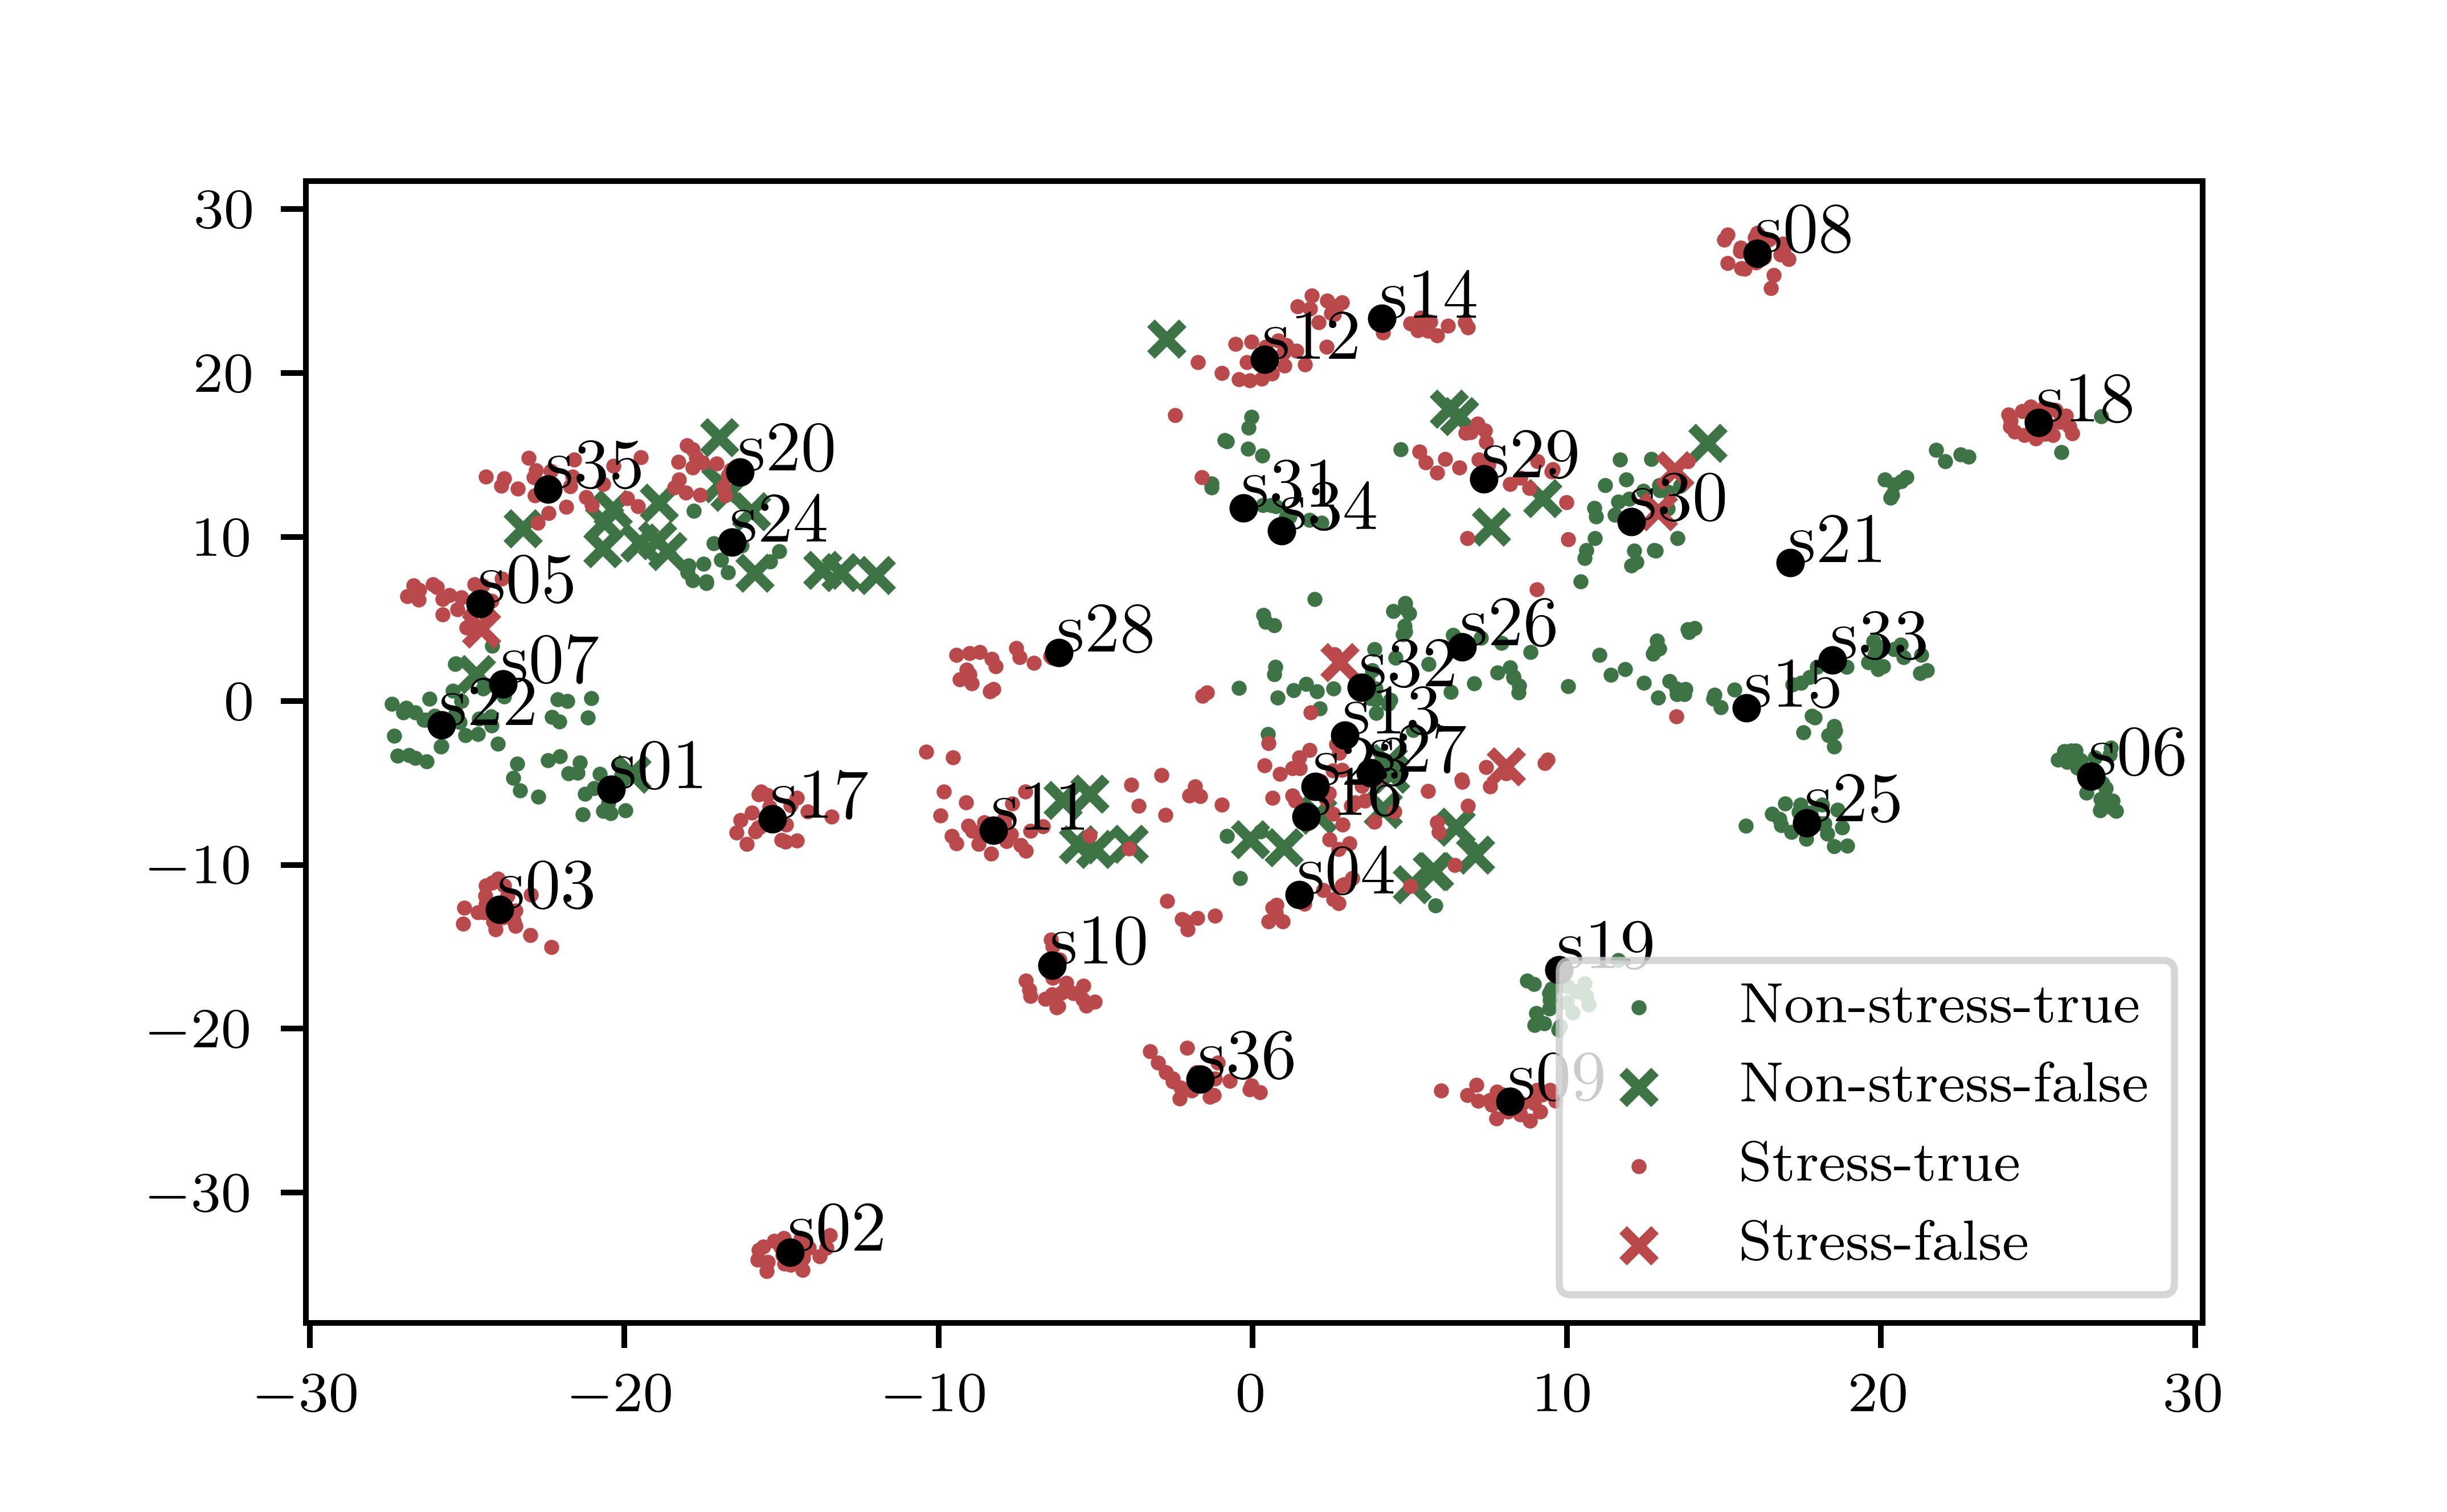
\includegraphics[width=1\textwidth]{figures/t-sne-baseline-8.png}
  }
  \label{fig:t-sne-bseline-8}
\end{figure}

\subsubsection{Logistic Regression Coefficient}

Table~\ref{tab:cv_LR} shows the result using the ranked features of Logistic Regression Coefficient. With this rank, the SVM is able to achieve 0.9 10-CV score at top six features. The LR classifier also reach 0.8 10-CV score at top nine features, seven features less than the $\text{Rank}_{\text{Baseline}}$. The top six features of $\text{Rank}_{\text{LR}}$ are $\text{F3}_{\beta}$, $\text{P4}_{\delta}$, $\beta_{f}$, $\text{C3}_{\text{RG}}$, $\text{F3}_{\delta}$, $\text{F4}_{\delta}$, and $\text{T4}_{\theta}$.

\begin{table}[h!]
\centering
\caption{The 10-CV score of each classifier when using $\text{Rank}_{\text{LR}}$ as a rank. The model is trained on a list of features from $\text{Rank}^1$ to $\text{Rank}^i$ where $i$ is the row number.}
\label{tab:cv_LR}
\begin{tabular}{r|cccc}
\hline
 No. &     $\text{Rank}_{\text{LR}}$ &  coeff &                      SVM &                       LR \\
\hline
   1 &           $\text{F3}_{\beta}$ &  1.894 &          0.575$\pm$0.051 &          0.558$\pm$0.040 \\
   2 &          $\text{P4}_{\delta}$ &  1.651 &          0.635$\pm$0.050 &          0.571$\pm$0.048 \\
   3 &                   $\beta_{f}$ & -1.435 &          0.749$\pm$0.058 &          0.624$\pm$0.051 \\
   4 &       $\text{C3}_{\text{RG}}$ & -1.346 &          0.858$\pm$0.034 &          0.646$\pm$0.032 \\
   5 &          $\text{F3}_{\delta}$ & -1.273 &          0.886$\pm$0.030 &          0.718$\pm$0.047 \\
   6 &          $\text{F4}_{\delta}$ & -1.258 & \textbf{0.900$\pm$0.042} &          0.735$\pm$0.061 \\
   7 &          $\text{T4}_{\theta}$ &  0.952 &          0.910$\pm$0.029 &          0.735$\pm$0.053 \\
   8 & $\text{F3}_{\text{Low}\beta}$ & -0.841 &          0.921$\pm$0.037 &          0.765$\pm$0.054 \\
   9 &          $\text{P4}_{\alpha}$ & -0.833 &          0.961$\pm$0.014 & \textbf{0.836$\pm$0.040} \\
  10 &          $\text{F7}_{\alpha}$ &  0.767 &          0.961$\pm$0.022 &          0.832$\pm$0.040 \\
  11 &          $\text{F4}_{\alpha}$ & -0.609 &          0.960$\pm$0.018 &          0.846$\pm$0.048 \\
  12 &          $\text{F3}_{\alpha}$ & -0.594 &          0.961$\pm$0.016 &          0.858$\pm$0.045 \\
  13 &         $\text{FP1}_{\delta}$ & -0.503 &          0.964$\pm$0.015 &          0.849$\pm$0.052 \\
  14 &          $\text{T6}_{\alpha}$ & -0.465 &          0.957$\pm$0.015 &          0.854$\pm$0.019 \\
  15 &          $\text{F3}_{\gamma}$ &  0.422 &          0.957$\pm$0.031 &          0.856$\pm$0.032 \\
  16 &          $\text{P4}_{\theta}$ &  0.405 &          0.971$\pm$0.018 &          0.851$\pm$0.049 \\
  17 & $\text{T4}_{\text{Low}\beta}$ &  0.396 &          0.968$\pm$0.019 &          0.850$\pm$0.041 \\
  18 &          $\text{F3}_{\theta}$ & -0.384 &          0.969$\pm$0.016 &          0.854$\pm$0.037 \\
  19 &          $\text{C3}_{\delta}$ &  0.350 &          0.982$\pm$0.013 &          0.846$\pm$0.036 \\
  20 &          $\text{C3}_{\theta}$ & -0.348 &          0.979$\pm$0.016 &          0.847$\pm$0.020 \\
  21 &          $\text{T3}_{\gamma}$ & -0.323 &          0.979$\pm$0.011 &          0.850$\pm$0.034 \\
  22 &                  $\alpha_{t}$ & -0.201 &          0.975$\pm$0.019 &          0.853$\pm$0.034 \\
  23 &                  $\alpha_{a}$ & -0.182 &          0.981$\pm$0.023 &          0.853$\pm$0.035 \\
  24 &                  $\alpha_{f}$ & -0.067 &          0.979$\pm$0.017 &          0.847$\pm$0.052 \\
  25 &       $\text{F3}_\text{slow}$ &  0.036 &          0.975$\pm$0.015 &          0.840$\pm$0.042 \\
\hline
\end{tabular}
\end{table}

\begin{figure}[h!]
    \caption{The top six features from $\text{Rank}_{\text{Baseline}}$ and $\text{Rank}_{\text{LR}}$ plot in t-SNE space. The two groups are better separated in the case of $\text{Rank}_{\text{LR}}$. }
    \label{fig:t-SNE_baseline-lr}
    
    \centering
    \begin{subfigure}[b]{0.49\textwidth}
        \centering
        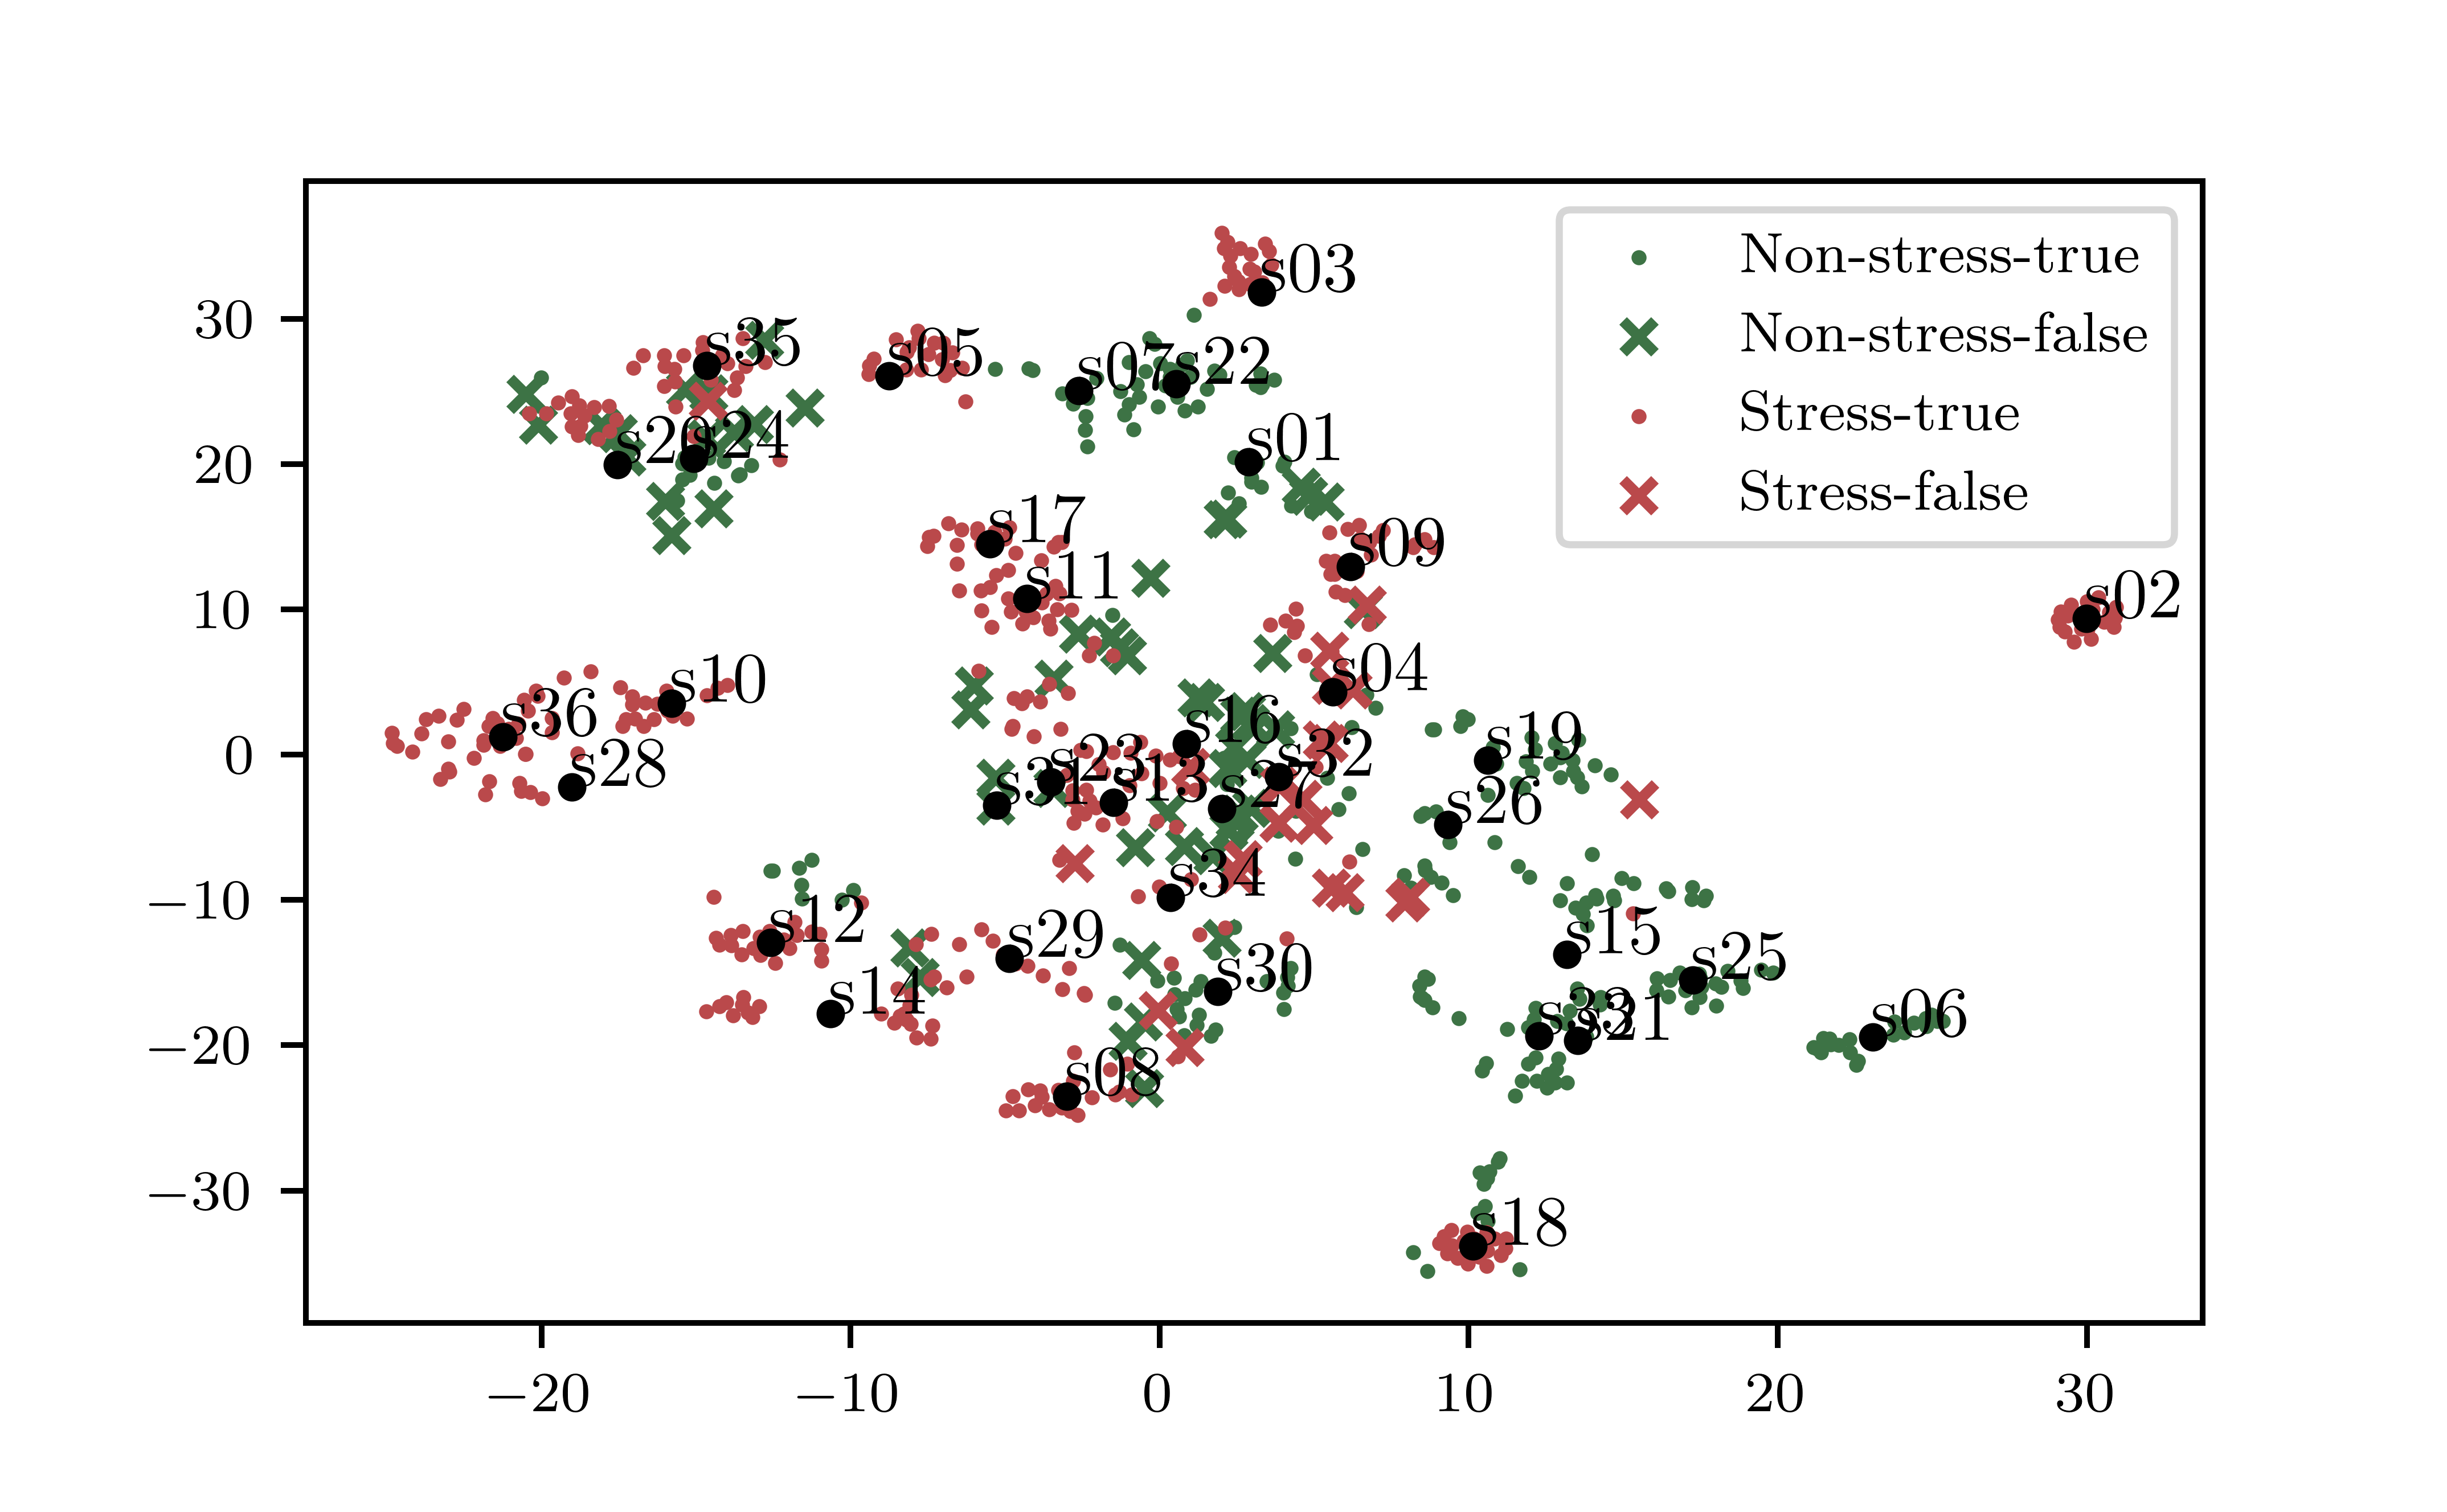
\includegraphics[width=\textwidth]{figures/t-sne-baseline-6.png}
        \caption{Baseline}
    \end{subfigure}
    \hfill
    \begin{subfigure}[b]{0.49\textwidth}
        \centering
        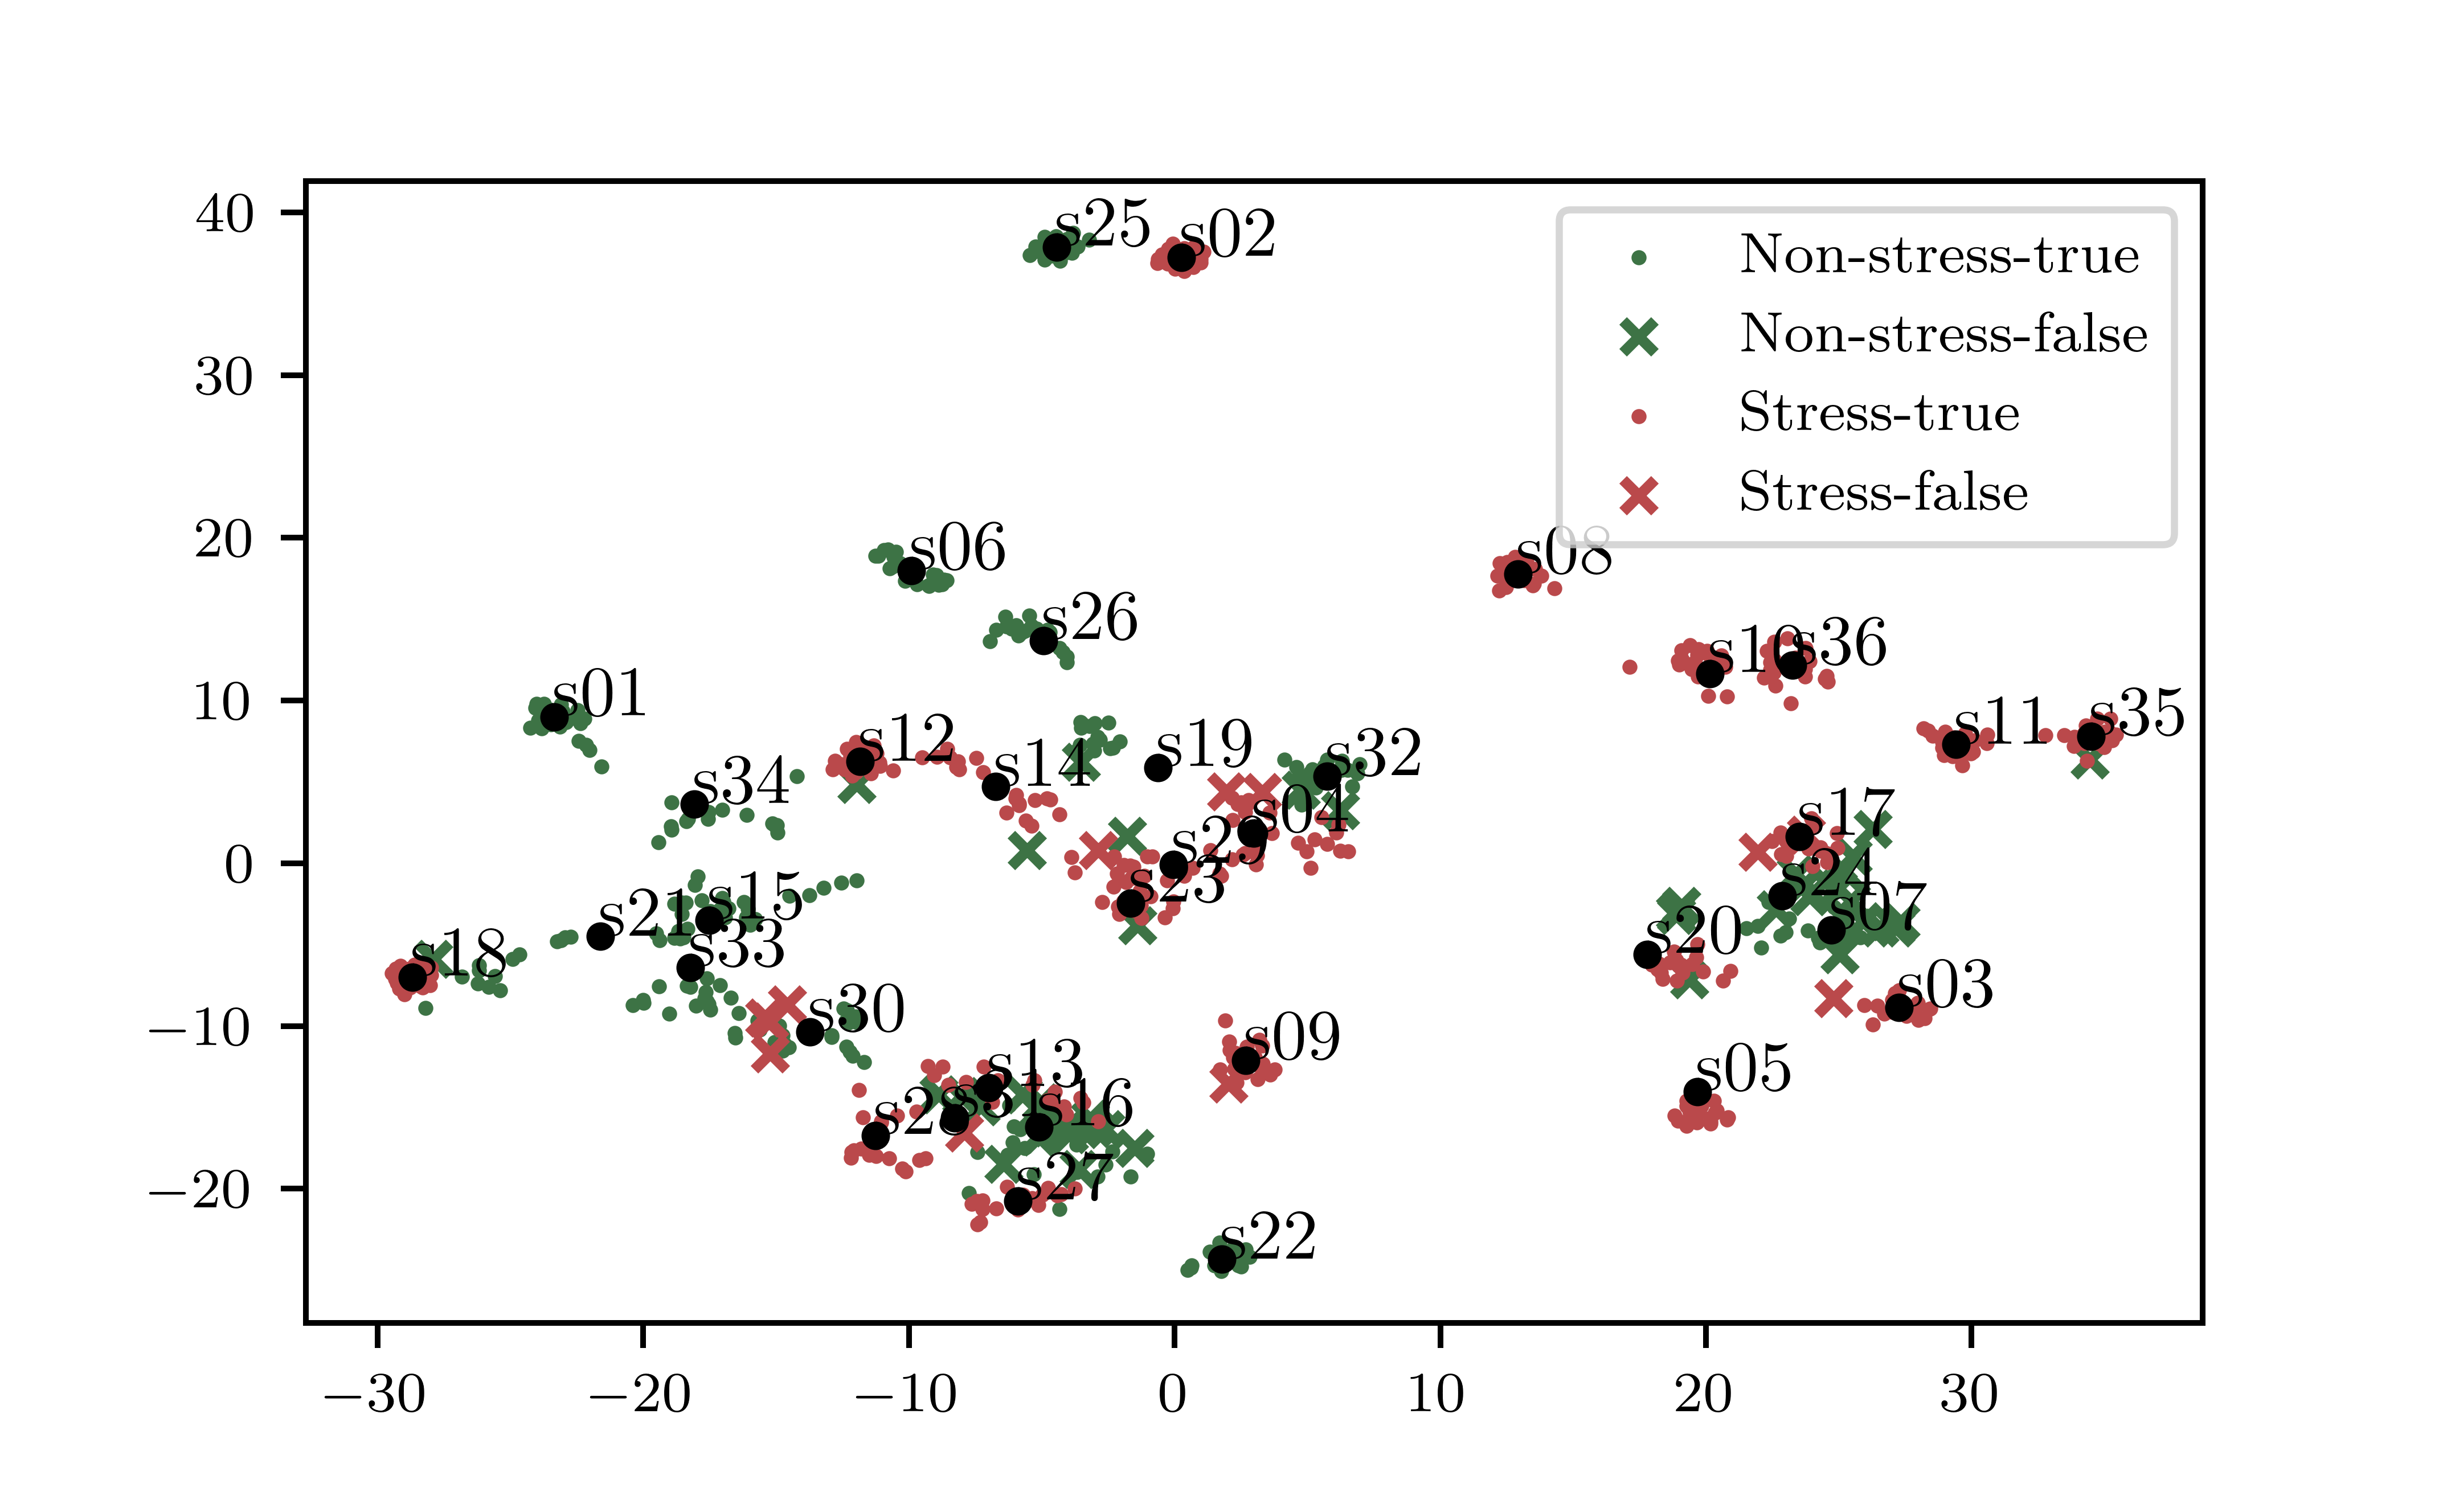
\includegraphics[width=\textwidth]{figures/t-sne-lr-6.png}
        \caption{LR}
    \end{subfigure}
\end{figure}

\subsubsection{Ensemble}

The score for $\text{Rank}_{\text{Ensemble}}$ is calculated follow the Equation~\ref{eq:rank_score}. Table~\ref{tab:cv_ensemble} shows the calculated score and rank them accordingly. In this configuration, SVM, at top six features, achieves $0.899\pm0.040$ 10-CV score and, later, achieves over 0.9 10-CV score at iteration eight. The top eight features are $\beta_{f}$, $\text{F3}_{\delta}$, $\text{F4}_{\delta}$, $\text{F3}_{\beta}$, $\text{P4}_{\delta}$, $\text{F3}_{\gamma}$, $\text{P4}_{\theta}$, and $\text{C3}_{\theta}$.

\begin{table}[h!]
\centering
\caption{The 10-CV score of each classifier when using $\text{Rank}_{\text{ensemble}}$ as a rank. The model is trained on a list of features from $\text{Rank}^1$ to $\text{Rank}^i$ where $i$ is the row number.}
\label{tab:cv_ensemble}
\begin{tabular}{r|cccc}
\hline
 No. & $\text{Rank}_{\text{ensemble}}$ &  score &                      SVM &                       LR \\
\hline
   1 &                     $\beta_{f}$ &     15 &          0.693$\pm$0.057 &          0.669$\pm$0.046 \\
   2 &            $\text{F3}_{\delta}$ &     18 &          0.765$\pm$0.029 &          0.731$\pm$0.048 \\
   3 &            $\text{F4}_{\delta}$ &     34 &          0.775$\pm$0.057 &          0.725$\pm$0.035 \\
   4 &             $\text{F3}_{\beta}$ &     34 &          0.849$\pm$0.040 &          0.743$\pm$0.047 \\
   5 &            $\text{P4}_{\delta}$ &     45 &          0.867$\pm$0.044 &          0.728$\pm$0.070 \\
   6 &            $\text{F3}_{\gamma}$ &     47 &          0.899$\pm$0.040 &          0.735$\pm$0.033 \\
   7 &            $\text{P4}_{\theta}$ &     48 &          0.890$\pm$0.040 &          0.754$\pm$0.041 \\
   8 &            $\text{C3}_{\theta}$ &     49 & \textbf{0.925$\pm$0.023} &          0.782$\pm$0.058 \\
   9 &         $\text{C3}_{\text{RG}}$ &     52 &          0.944$\pm$0.030 &          0.775$\pm$0.030 \\
  10 &            $\text{T4}_{\theta}$ &     54 &          0.947$\pm$0.017 &          0.794$\pm$0.050 \\
  11 &   $\text{T4}_{\text{Low}\beta}$ &     54 &          0.958$\pm$0.023 &          0.797$\pm$0.058 \\
  12 &            $\text{P4}_{\alpha}$ &     57 &          0.971$\pm$0.020 & \textbf{0.811$\pm$0.060} \\
  13 &            $\text{F7}_{\alpha}$ &     57 &          0.975$\pm$0.025 &          0.815$\pm$0.050 \\
  14 &            $\text{F3}_{\alpha}$ &     59 &          0.972$\pm$0.025 &          0.838$\pm$0.040 \\
  15 &            $\text{F3}_{\theta}$ &     61 &          0.976$\pm$0.021 &          0.849$\pm$0.034 \\
  16 &            $\text{C3}_{\delta}$ &     61 &          0.978$\pm$0.023 &          0.849$\pm$0.058 \\
  17 &            $\text{F4}_{\alpha}$ &     67 &          0.978$\pm$0.015 &          0.844$\pm$0.056 \\
  18 &   $\text{F3}_{\text{Low}\beta}$ &     69 &          0.979$\pm$0.018 &          0.849$\pm$0.036 \\
  19 &            $\text{T3}_{\gamma}$ &     71 &          0.981$\pm$0.013 &          0.840$\pm$0.035 \\
  20 &            $\text{T6}_{\alpha}$ &     73 &          0.981$\pm$0.015 &          0.850$\pm$0.053 \\
  21 &           $\text{FP1}_{\delta}$ &     79 &          0.979$\pm$0.009 &          0.844$\pm$0.037 \\
  22 &         $\text{F3}_\text{slow}$ &     88 &          0.981$\pm$0.013 &          0.844$\pm$0.040 \\
  23 &                    $\alpha_{f}$ &     94 &          0.981$\pm$0.011 &          0.854$\pm$0.036 \\
  24 &                    $\alpha_{a}$ &    103 &          0.979$\pm$0.013 &          0.850$\pm$0.038 \\
  25 &                    $\alpha_{t}$ &    111 &          0.978$\pm$0.015 &          0.844$\pm$0.020 \\
\hline
\end{tabular}
\end{table}

\begin{figure}[h!]
    \caption{The top six and top eight features from $\text{Rank}_{\text{LR}}$ and $\text{Rank}_{\text{Ensemble}}$ plot in t-SNE space.}
    \label{fig:t-SNE_lr-ensemble}
    
    \centering
    \begin{subfigure}[b]{0.49\textwidth}
        \centering
        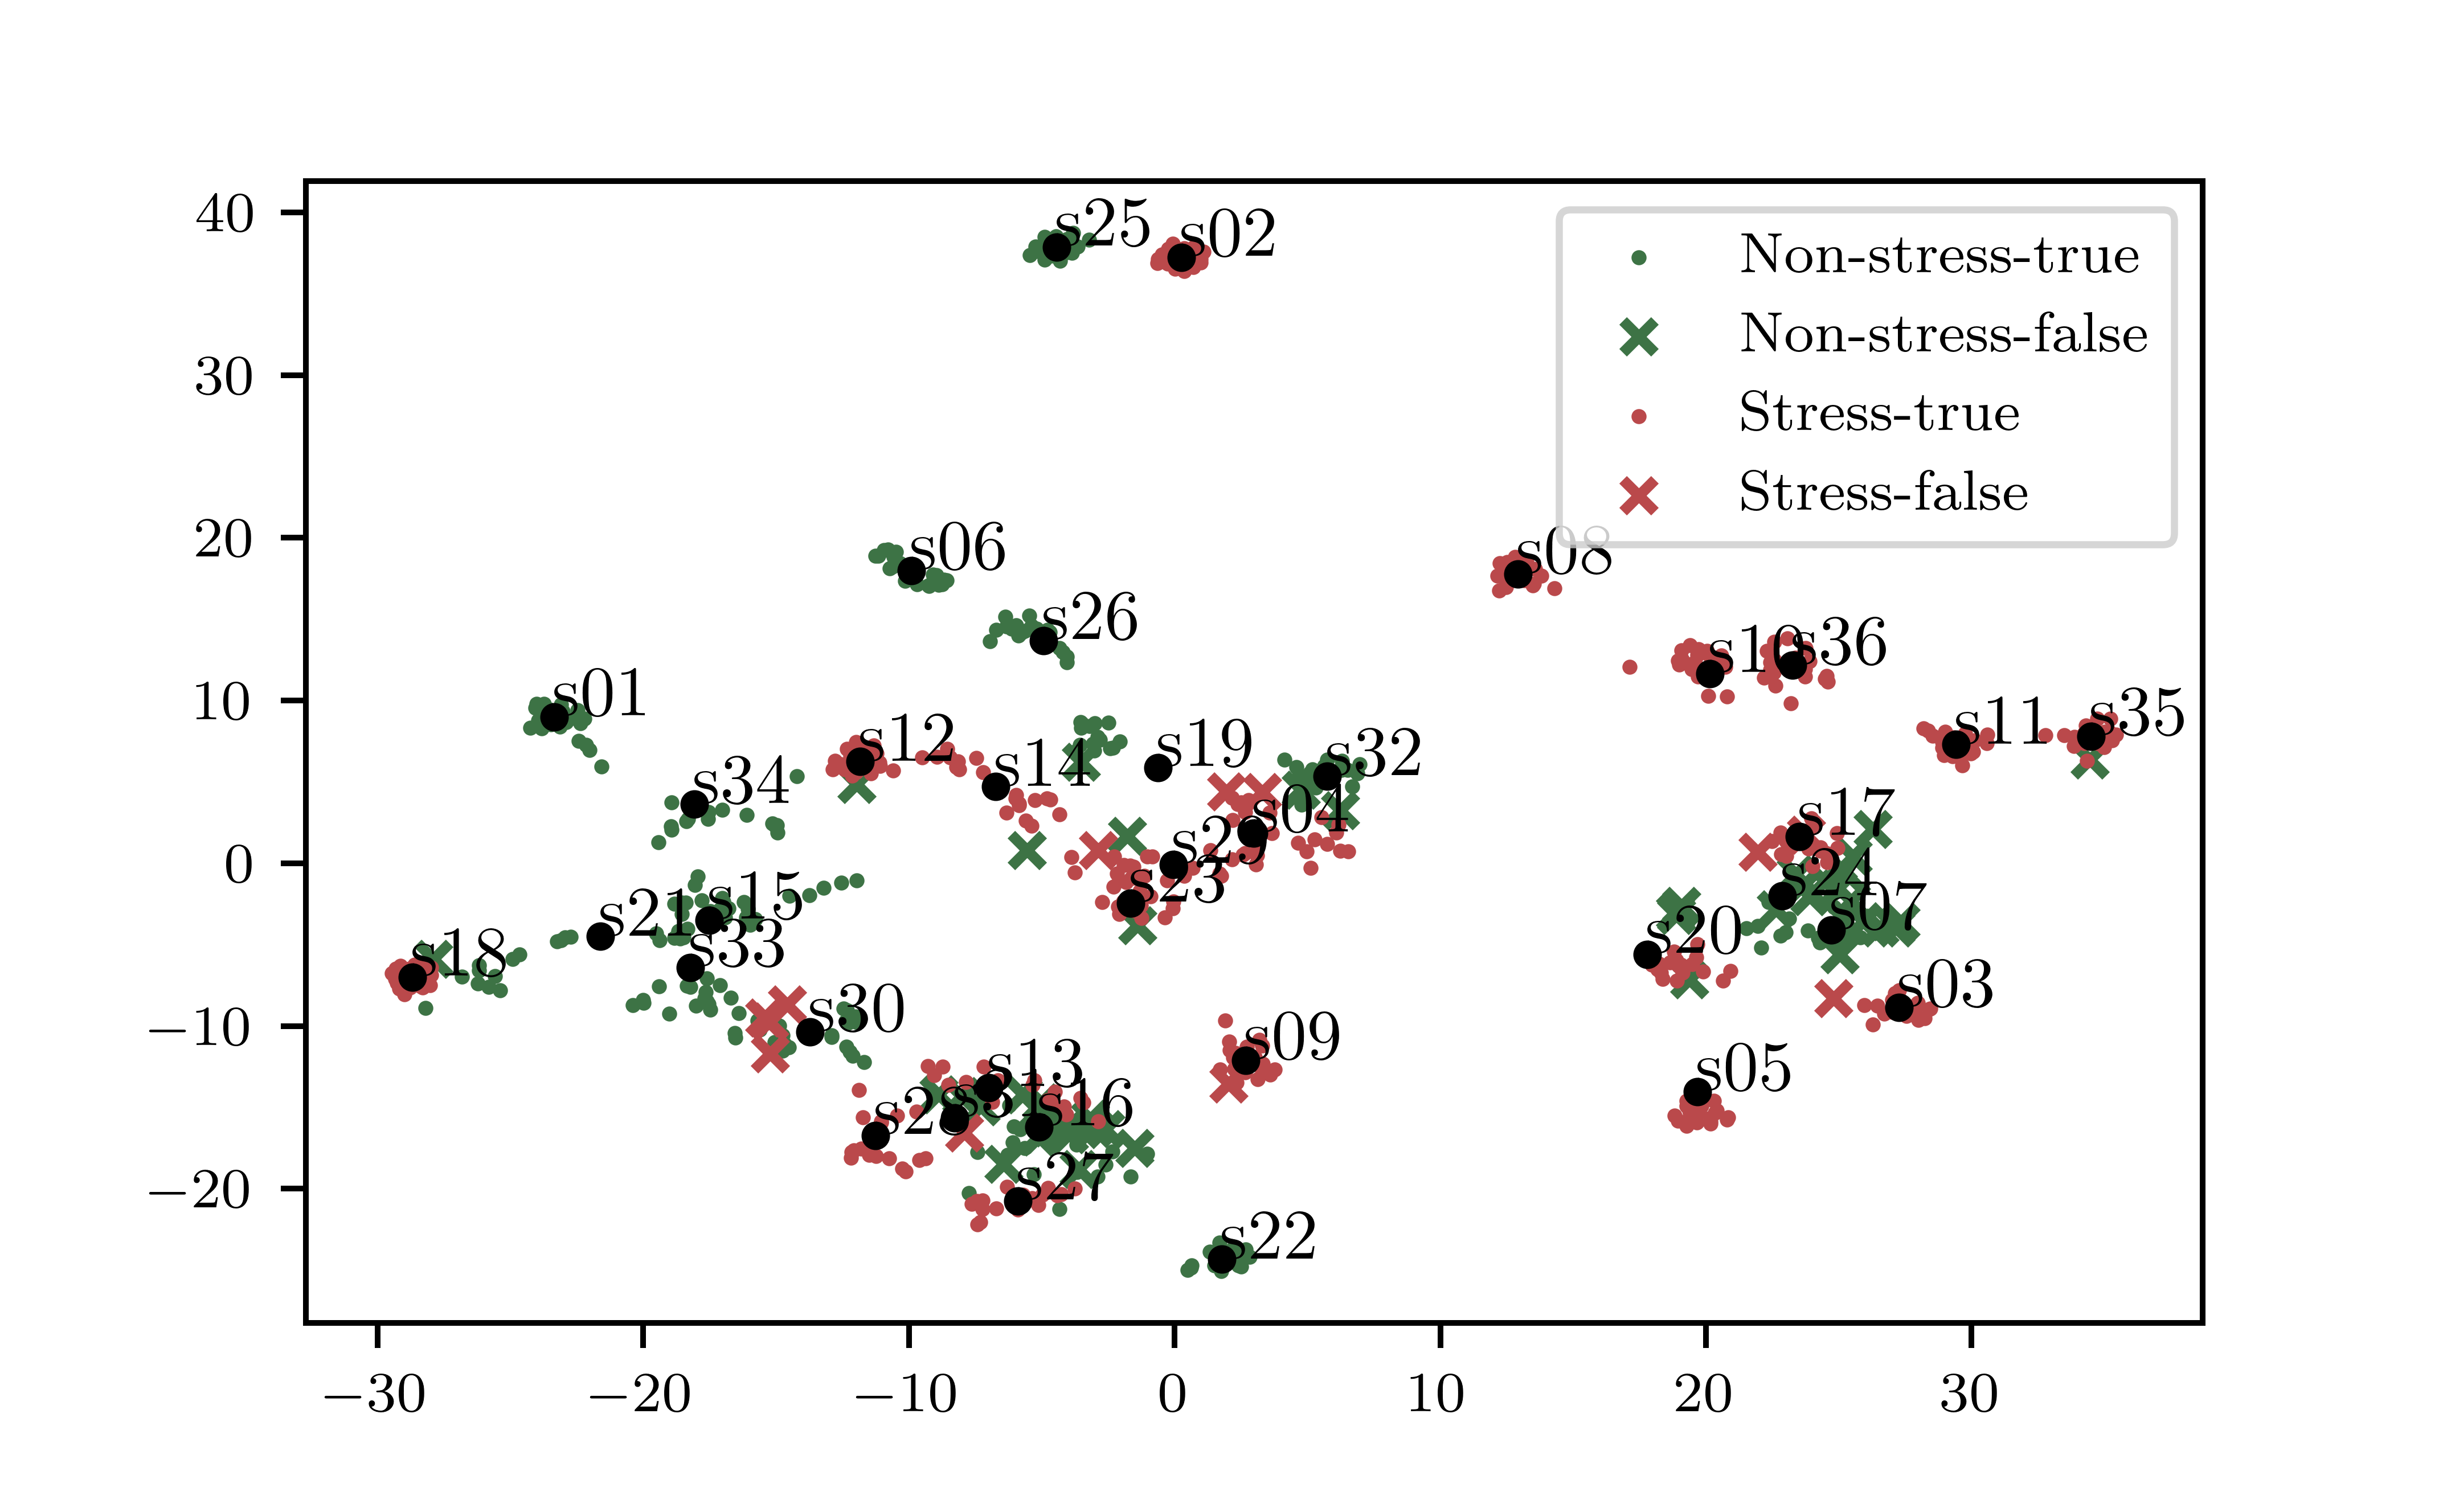
\includegraphics[width=\textwidth]{figures/t-sne-lr-6.png}
        \caption{top six LR}
    \end{subfigure}
    \hfill
    \begin{subfigure}[b]{0.49\textwidth}
        \centering
        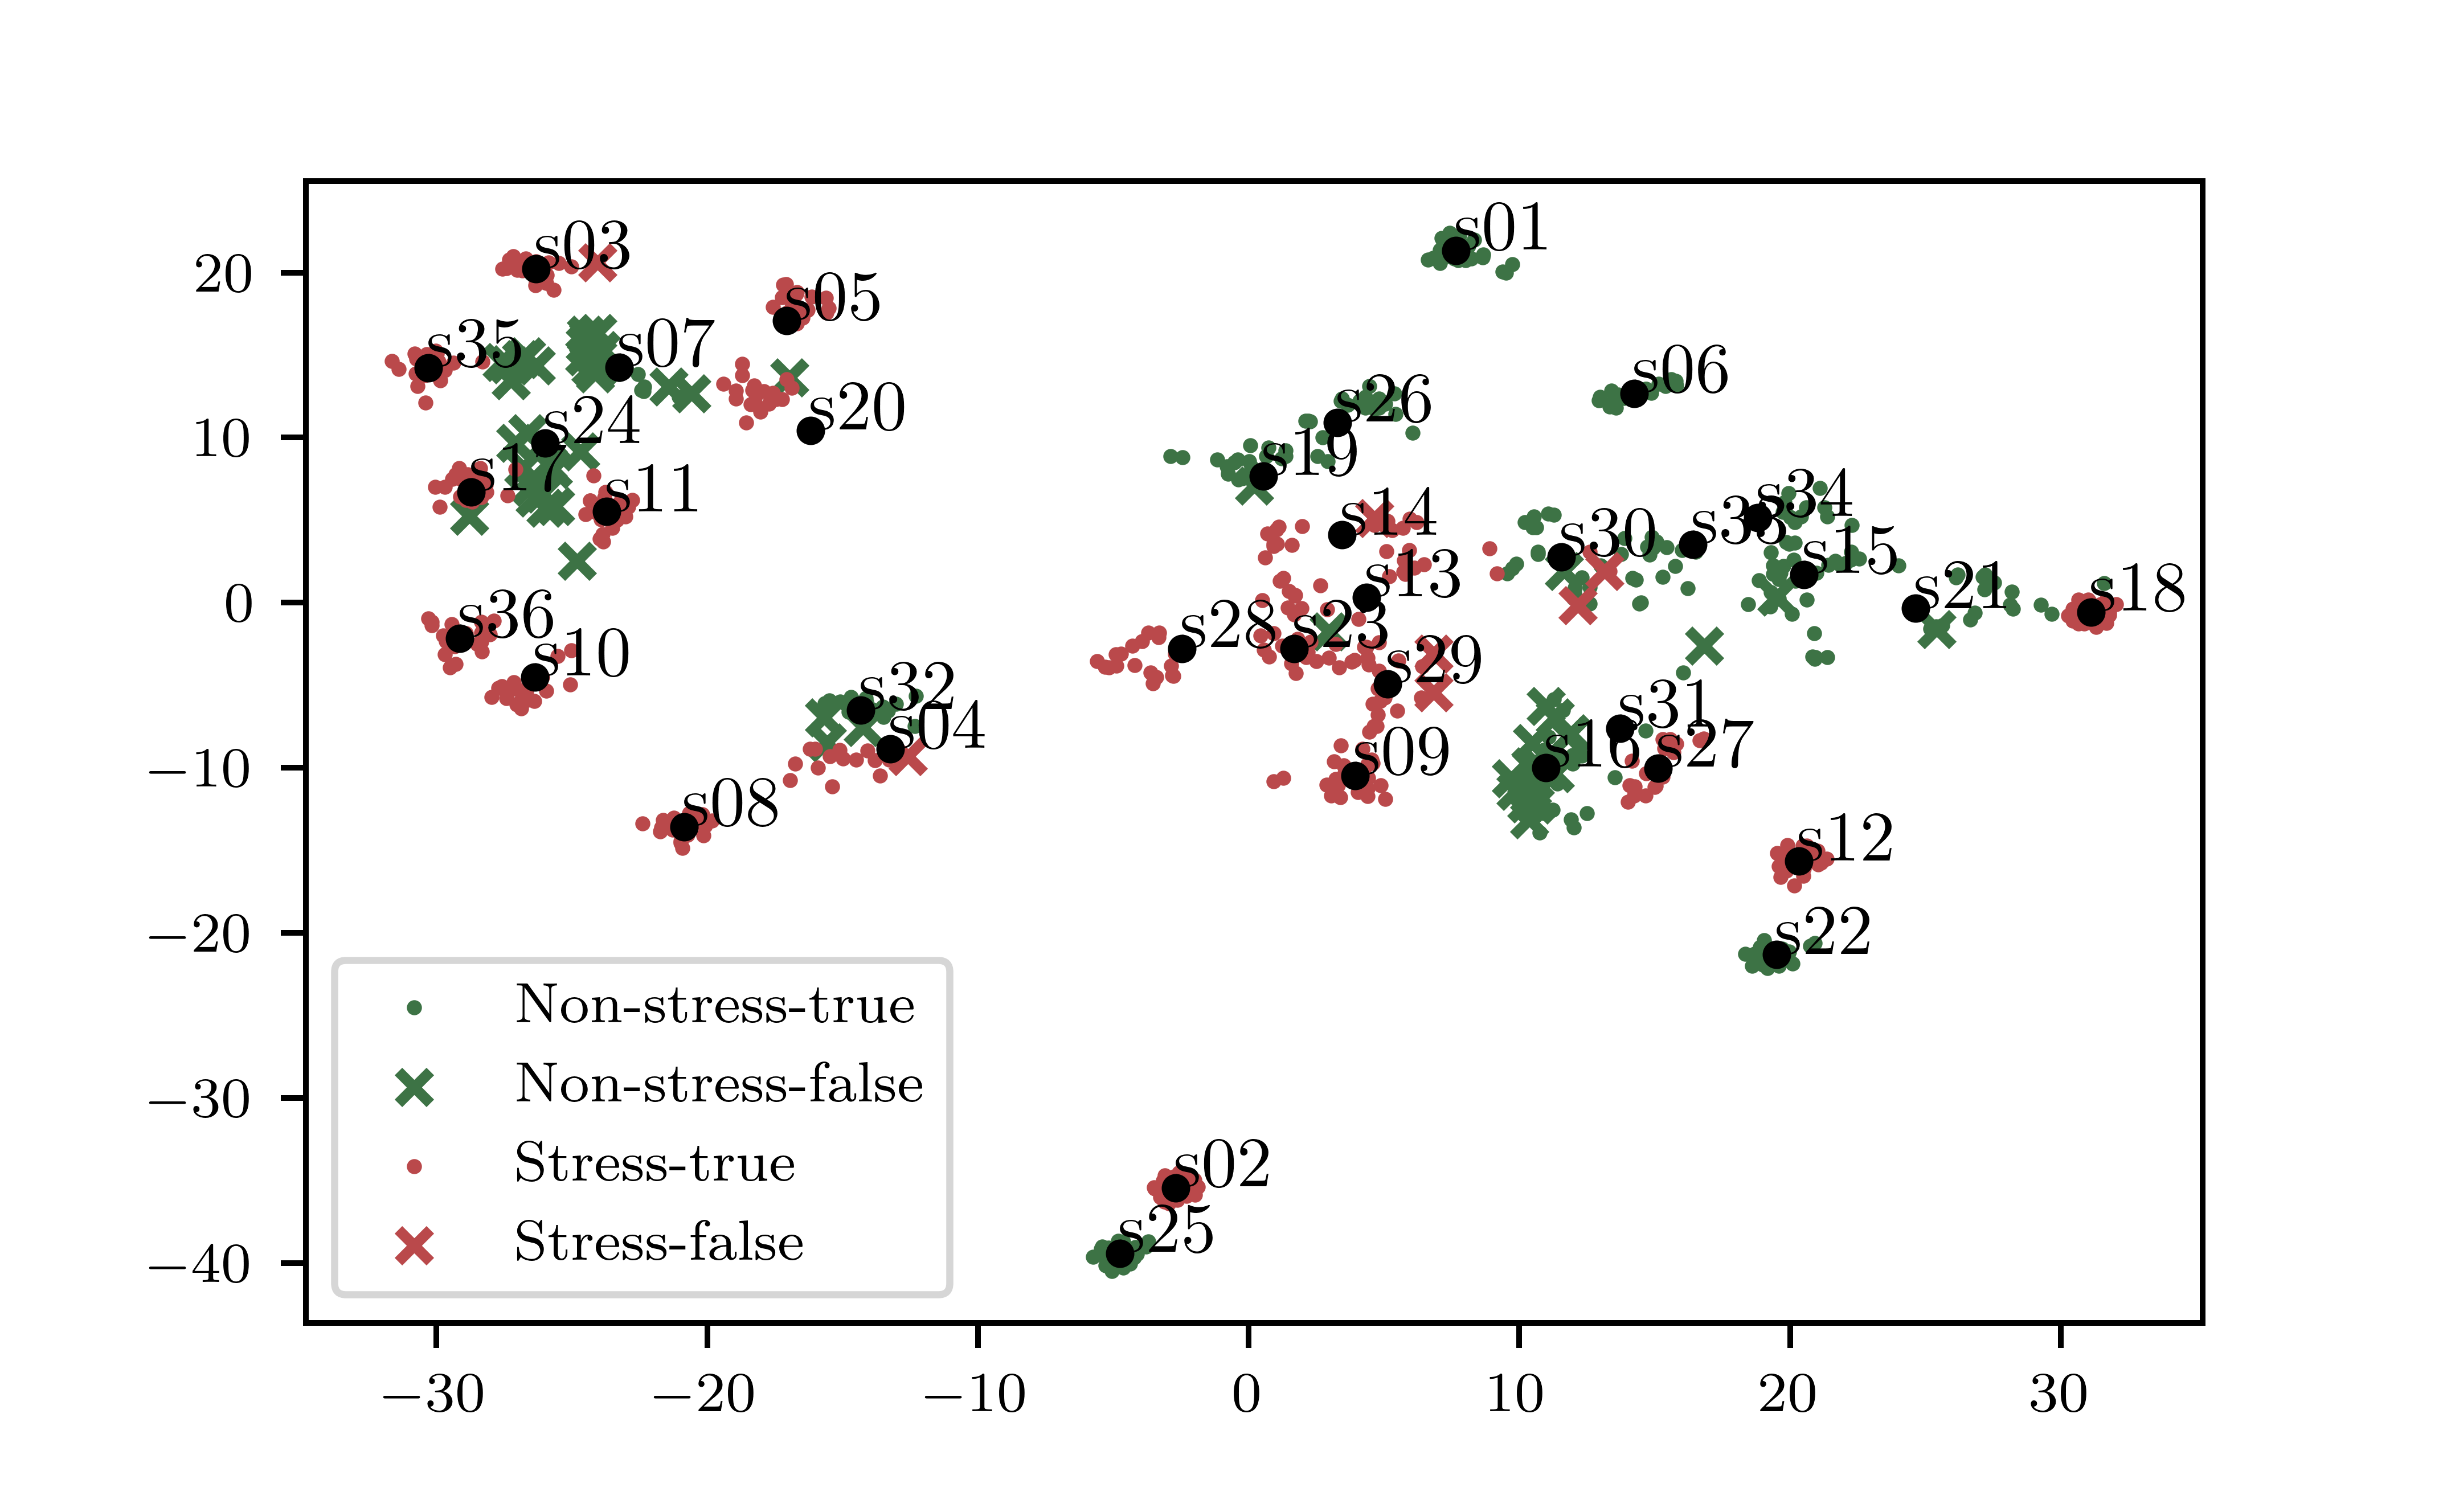
\includegraphics[width=\textwidth]{figures/t-sne-ensemble-6.png}
        \caption{top six Ensemble}
    \end{subfigure}
    \\
    \begin{subfigure}[b]{0.49\textwidth}
        \centering
        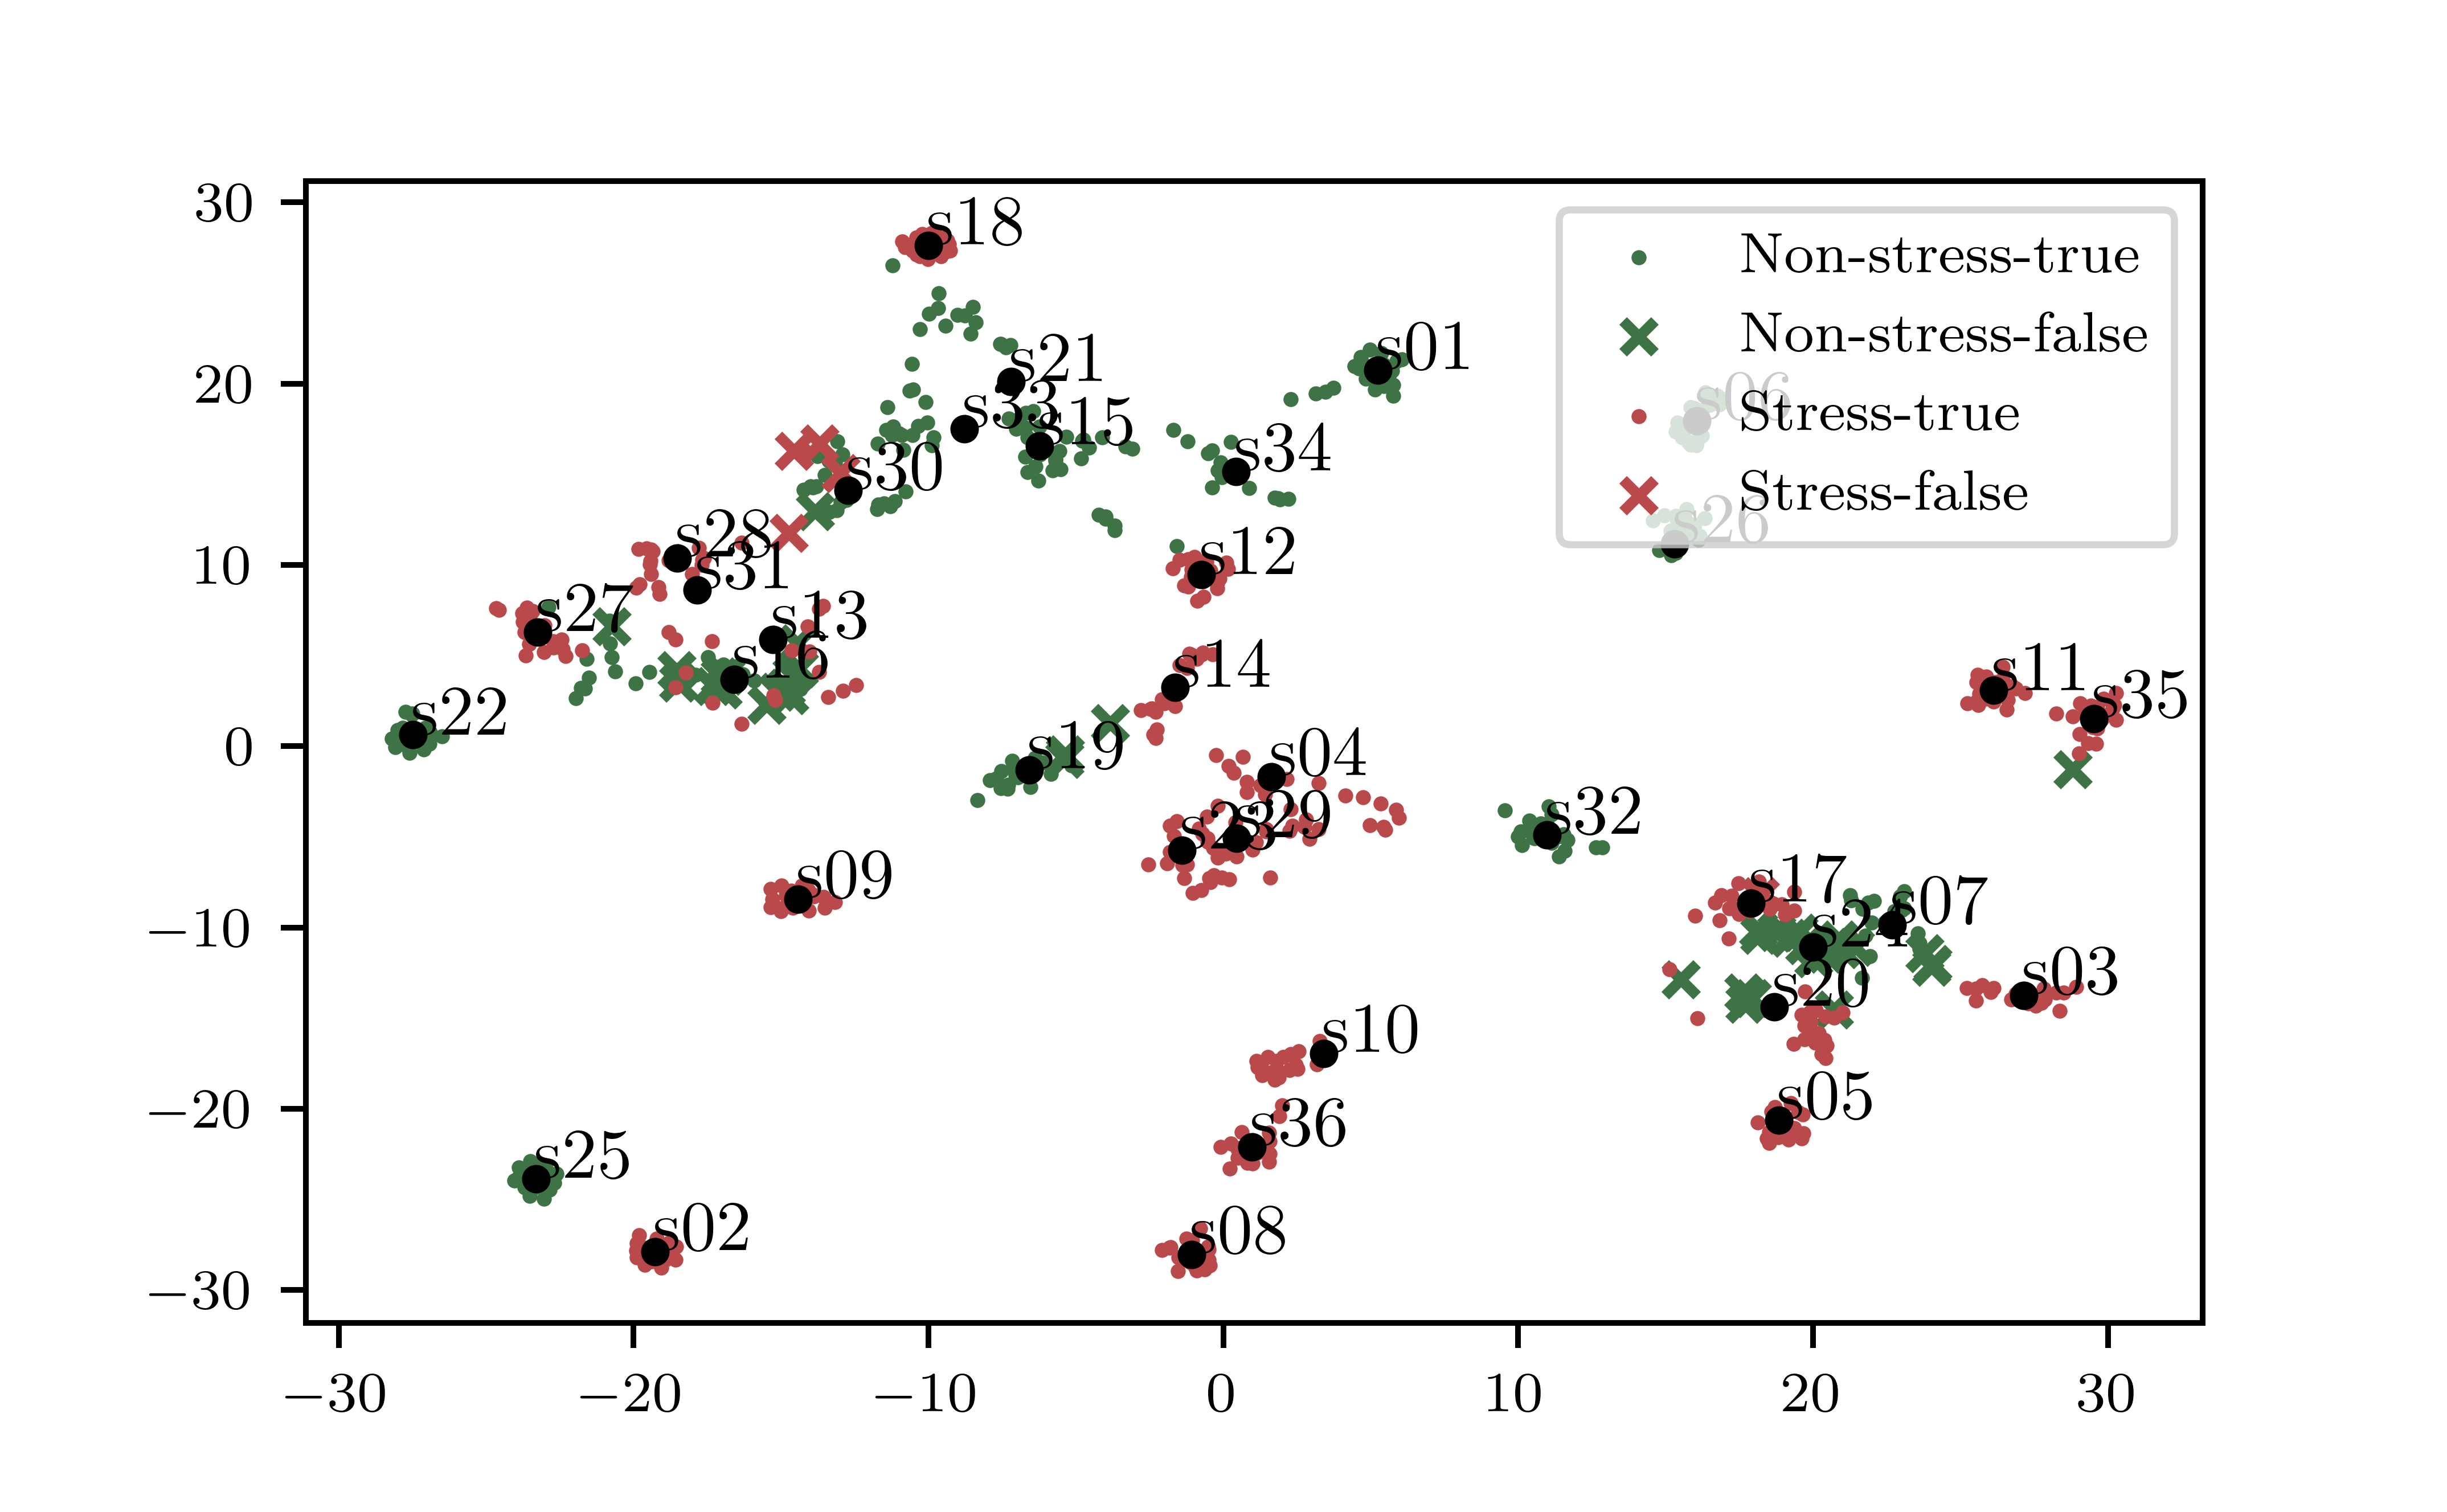
\includegraphics[width=\textwidth]{figures/t-sne-lr-8.png}
        \caption{top eight LR}
    \end{subfigure}
    \hfill
    \begin{subfigure}[b]{0.49\textwidth}
        \centering
        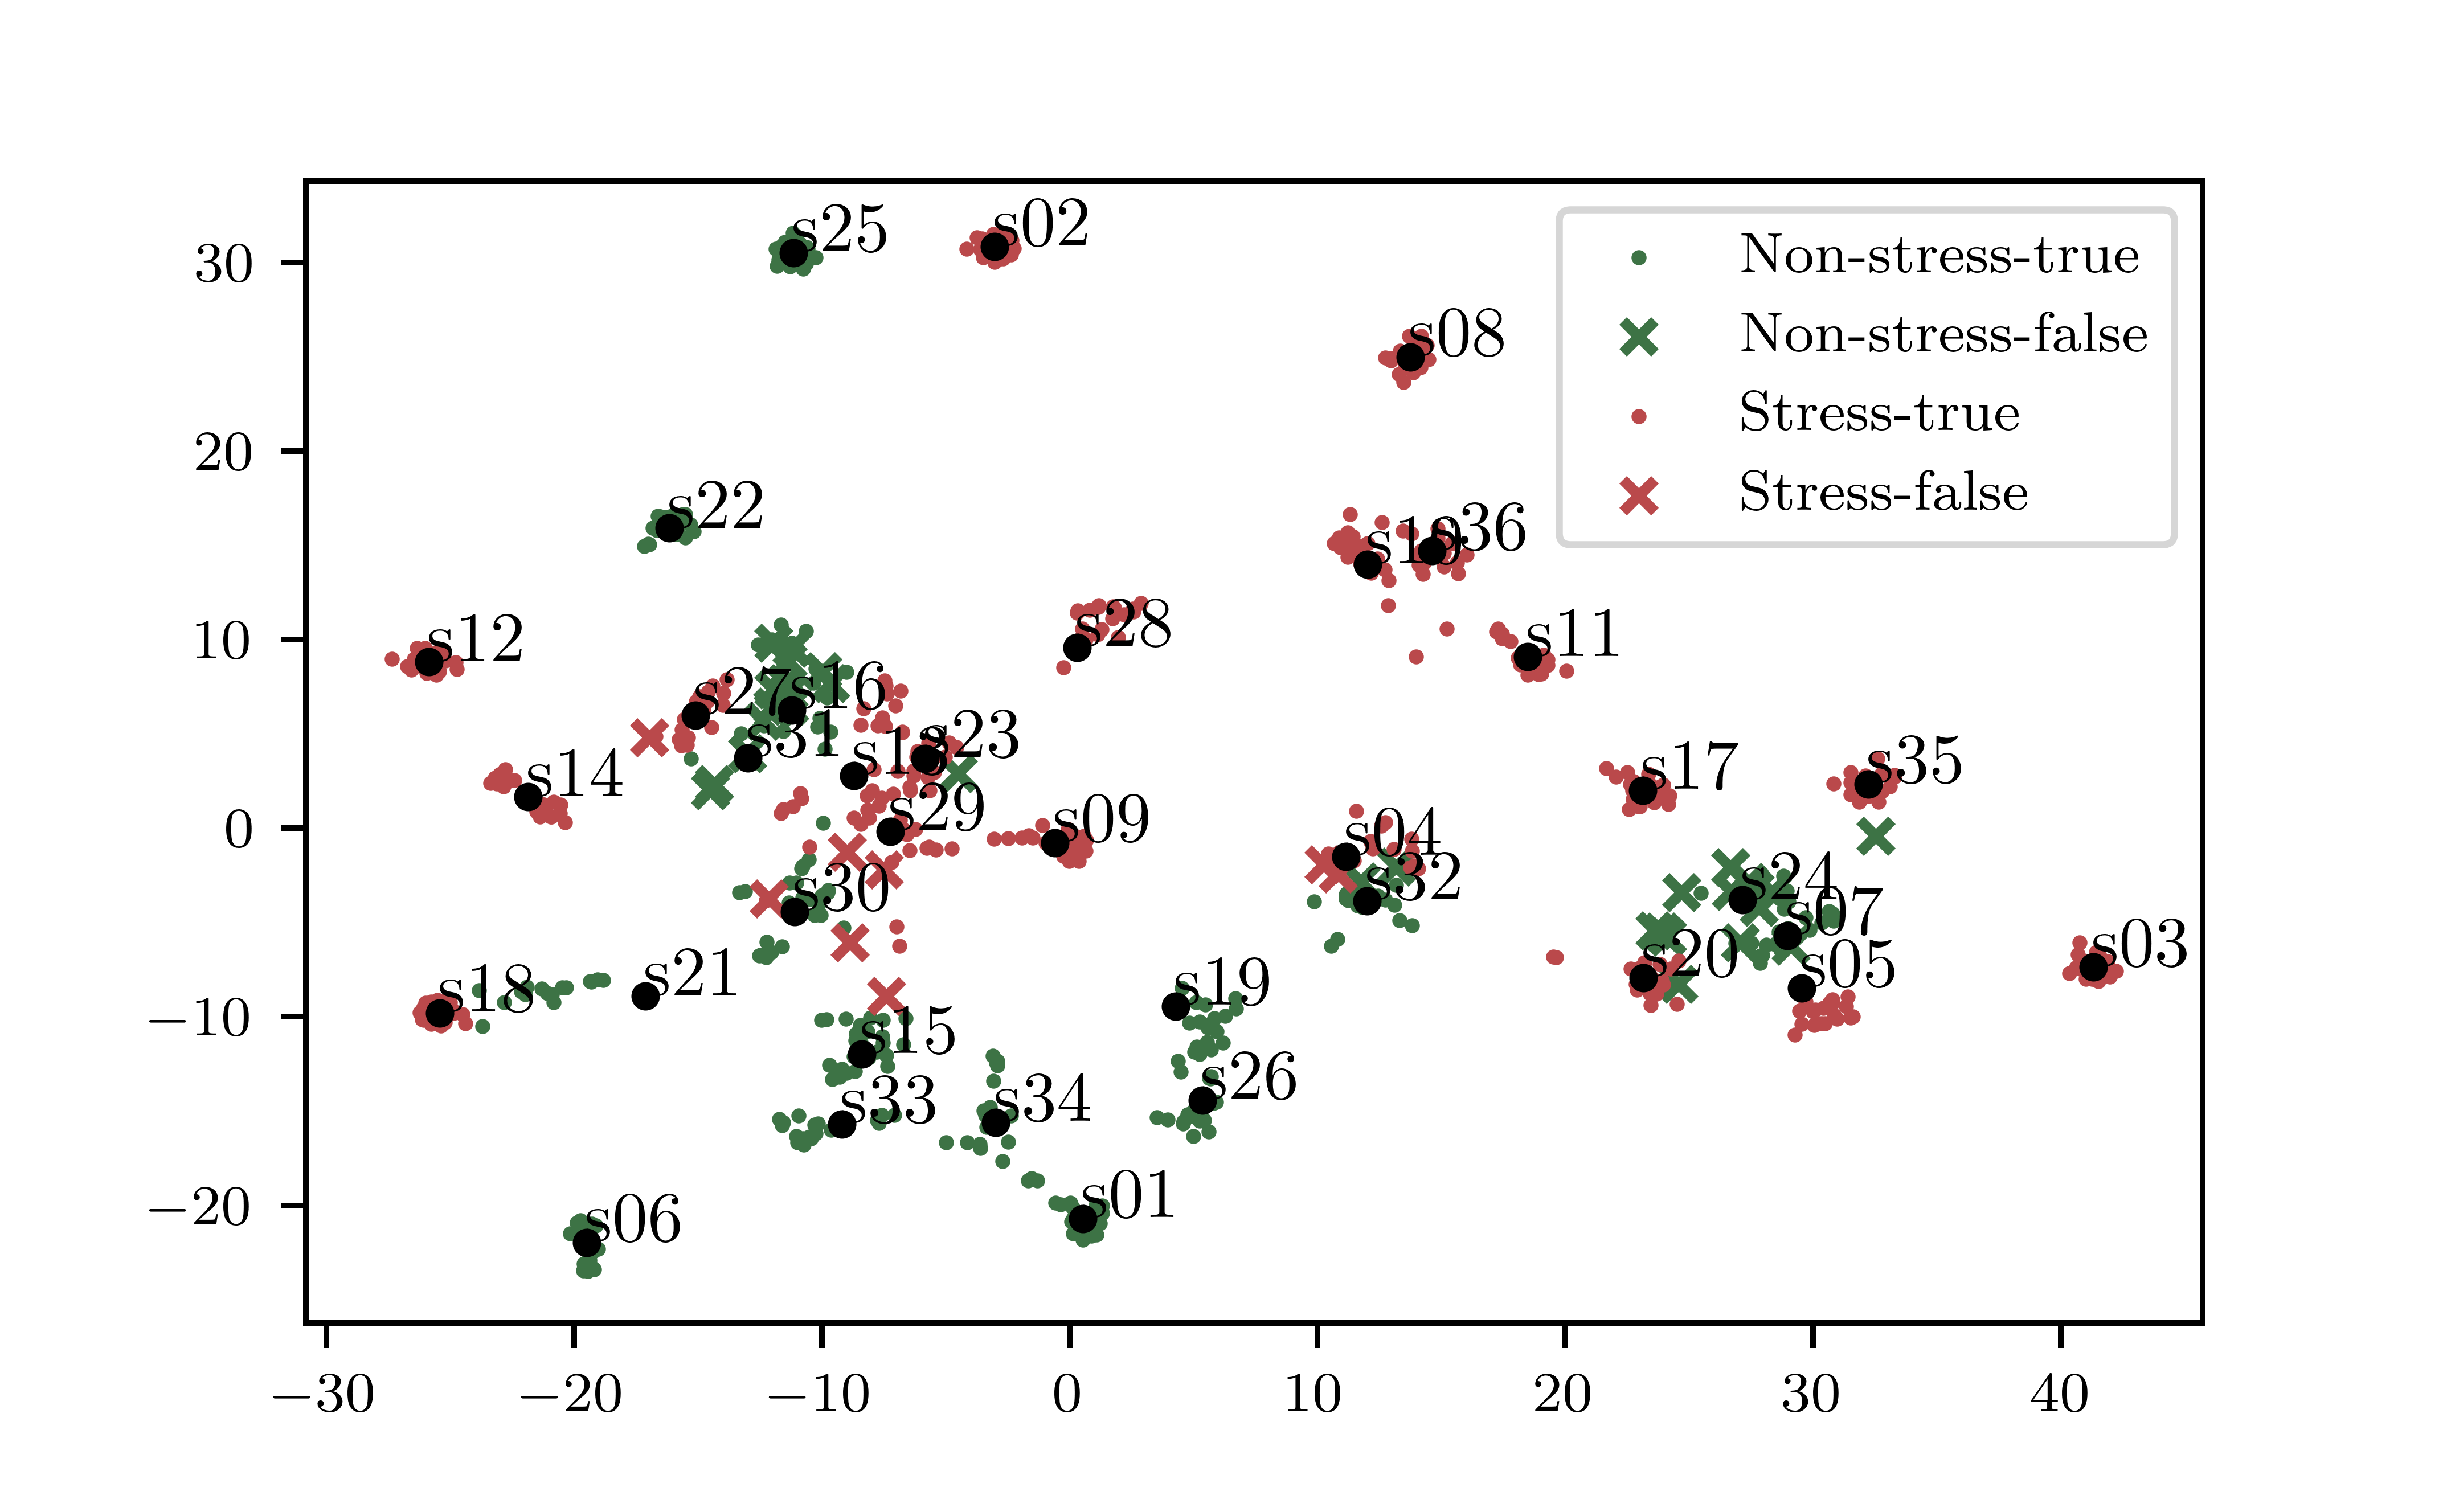
\includegraphics[width=\textwidth]{figures/t-sne-ensemble-8.png}
        \caption{top eight Ensemble}
    \end{subfigure}
\end{figure}

\FloatBarrier

\section{Discussion}\label{sec5}

At the recording state, we chose to do eye-closed conditions because we want to avoid external factors such as lighting conditions and visual distraction, as well as eye artifacts. However, there are challenges to this approach. First, during closing the eye, the power of the Alpha band in the occipital area is greatly increased. We could argue that this does not affect our result but due to the nature of EEG, the Alpha information in the occipital area could contaminate their neighbor. Maybe this is the reason why any of the Alpha asymmetry features are staying at the bottom of the rank. Second, the participant might fall asleep during the record. Because the record session is five minutes long and the participant is asked to avoid any form of caffeine which many of them have on a daily basis, closing the eyes for five minutes is enough to turn some participants into a relaxing or sleeping state. 

All 55 participants can be considered well educated since all of them are, at least, pursuing a degree of bachelor. The nationality range is limited to Asian and the age is between 20 and 40 years old. Our data is somewhat biased by this fact. 

The label of the data is based on the questionnaire PSS-10 score, a method subject to error and manipulation. The analysis could be improved if a psychologist expert is involved in the labeling process. Because of our labeling method, our data has a minor imbalance issue which we chose to ignore (16 Non-stress and 20 Stress participants). Our suggestion would be to increase the lower threshold to accommodate more Non-stress samples or we could segment the two groups differently.

In our experiment, RBF-SVM shows to be the best classifier for chronic stress. However, because of the nature of the RBF kernel, we can not rank the features by importance. To be specific, given enough data dimension, RBF-SVM always achieves a 0.9 10-CV score. While we could brute force through every combination of features given enough time, we can not be sure that the model learns chronic stress patterns or participant-specific patterns. Because of this reason, t-SNE is utilized. 

We, first, investigated the Logistic Regression Coefficient and found that, in t-SNE space, the two groups are well separated as shown in Figure~\ref{fig:t-SNE_baseline-lr}. In addition, the performance of other models is also improved given a smaller set of features (Table~\ref{tab:cv_lr_apen}). Therefore, we extend our idea to other models and, finally, convolute all ranks into the $\text{Rank}_{\text{Ensemble}}$. Every classifier seems to agree that the Beta and Delta band are the most important frequency. The electrode $\text{F3}$ is the most important followed by $\text{F4}$ and $\text{P4}$. Our result agrees with the previous studies \cite{Saeed2020}

Furthermore, t-SNE plots seem to suggest that our data has an outlier, for instance, s07 and s24 consistently appear in the middle of the stress group. To confirm this assumption, a larger and broader group of participants is needed. 

\section{Conclusion}\label{sec6}

In conclusion, the rest-state EEG can be used to classify chronic stress. The classification result shows that SVM with rbf kernel achieves over 0.98 10-CV scores and LR achieves 0.85 using all features with $p < .001$ from the reported t-test result. Extended ranking with various classifiers improve the feature selection and help to narrow down the feature list. Finally, convoluted $\text{Rank}_{\text{Ensemble}}$ shows the top eight Chronic Stress features which are $\beta_{f}$, $\text{F3}_{\delta}$, $\text{F4}_{\delta}$, $\text{F3}_{\beta}$, $\text{P4}_{\delta}$, $\text{F3}_{\gamma}$, $\text{P4}_{\theta}$, and $\text{C3}_{\theta}$. With these eight features, rbf-SVM, ADA, GB, and RF achieve over 0.9 10-CV score while adding the next four features ( $\text{C3}_{\text{RG}}$, $\text{T4}_{\theta}$, $\text{T4}_{\text{Low}\beta}$, and $\text{P4}_{\alpha}$ ), helps LR and LDA to achieve over 0.8 10-CV score (Table~\ref{tab:cv_ensemble_apen}). 

%\backmatter

%\bmhead{Supplementary information}

%If your article has accompanying supplementary file/s please state so here. 

%Authors reporting data from electrophoretic gels and blots should supply the full unprocessed scans for key as part of their Supplementary information. This may be requested by the editorial team/s if it is missing.

%Please refer to Journal-level guidance for any specific requirements.

%\bmhead{Acknowledgments}

%Acknowledgments are not compulsory. Where included they should be brief. Grant or contribution numbers may be acknowledged.

%Please refer to Journal-level guidance for any specific requirements.

%\section*{Declarations}

%Some journals require declarations to be submitted in a standardised format. Please check the Instructions for Authors of the journal to which you are submitting to see if you need to complete this section. If yes, your manuscript must contain the following sections under the heading `Declarations':

%\begin{itemize}
%\item Funding
%\item Conflict of interest/Competing interests (check journal-specific guidelines for which heading to use)
%\item Ethics approval 
%\item Consent to participate
%\item Consent for publication
%\item Availability of data and materials
%\item Code availability 
%\item Authors' contributions
%\end{itemize}

%\noindent
%If any of the sections are not relevant to your manuscript, please include the heading and write `Not applicable' for that section. 

%%===================================================%%
%% For presentation purpose, we have included        %%
%% \bigskip command. please ignore this.             %%
%%===================================================%%
\bigskip
\newpage
%\begin{flushleft}%
%Editorial Policies for:

%\bigskip\noindent
%Springer journals and proceedings: %\url{https://www.springer.com/gp/editorial-policies}

%\bigskip\noindent
%Nature Portfolio journals: %\url{https://www.nature.com/nature-research/editorial-policies}

%\bigskip\noindent
%\textit{Scientific Reports}: %\url{https://www.nature.com/srep/journal-policies/editorial-policies}

%\bigskip\noindent
%BMC journals: \url{https://www.biomedcentral.com/getpublished/editorial-policies}
%\end{flushleft}

\begin{appendices}

%\section{Section title of first appendix}\label{secA1}

%An appendix contains supplementary information that is not an essential part of the text itself but which may be helpful in providing a more comprehensive understanding of the research problem or it is information that is too cumbersome to be included in the body of the paper.

%%=============================================%%
%% For submissions to Nature Portfolio Journals %%
%% please use the heading ``Extended Data''.   %%
%%=============================================%%

%%=============================================================%%
%% Sample for another appendix section			       %%
%%=============================================================%%

%% \section{Example of another appendix section}\label{secA2}%
%% Appendices may be used for helpful, supporting or essential material that would otherwise 
%% clutter, break up or be distracting to the text. Appendices can consist of sections, figures, 
%% tables and equations etc.

\section{10-CV result of each Ranks}\label{apen:ranks}

\begin{figure}[h!]
  \centering
  \caption{A bump chart of features in each ranking.}
  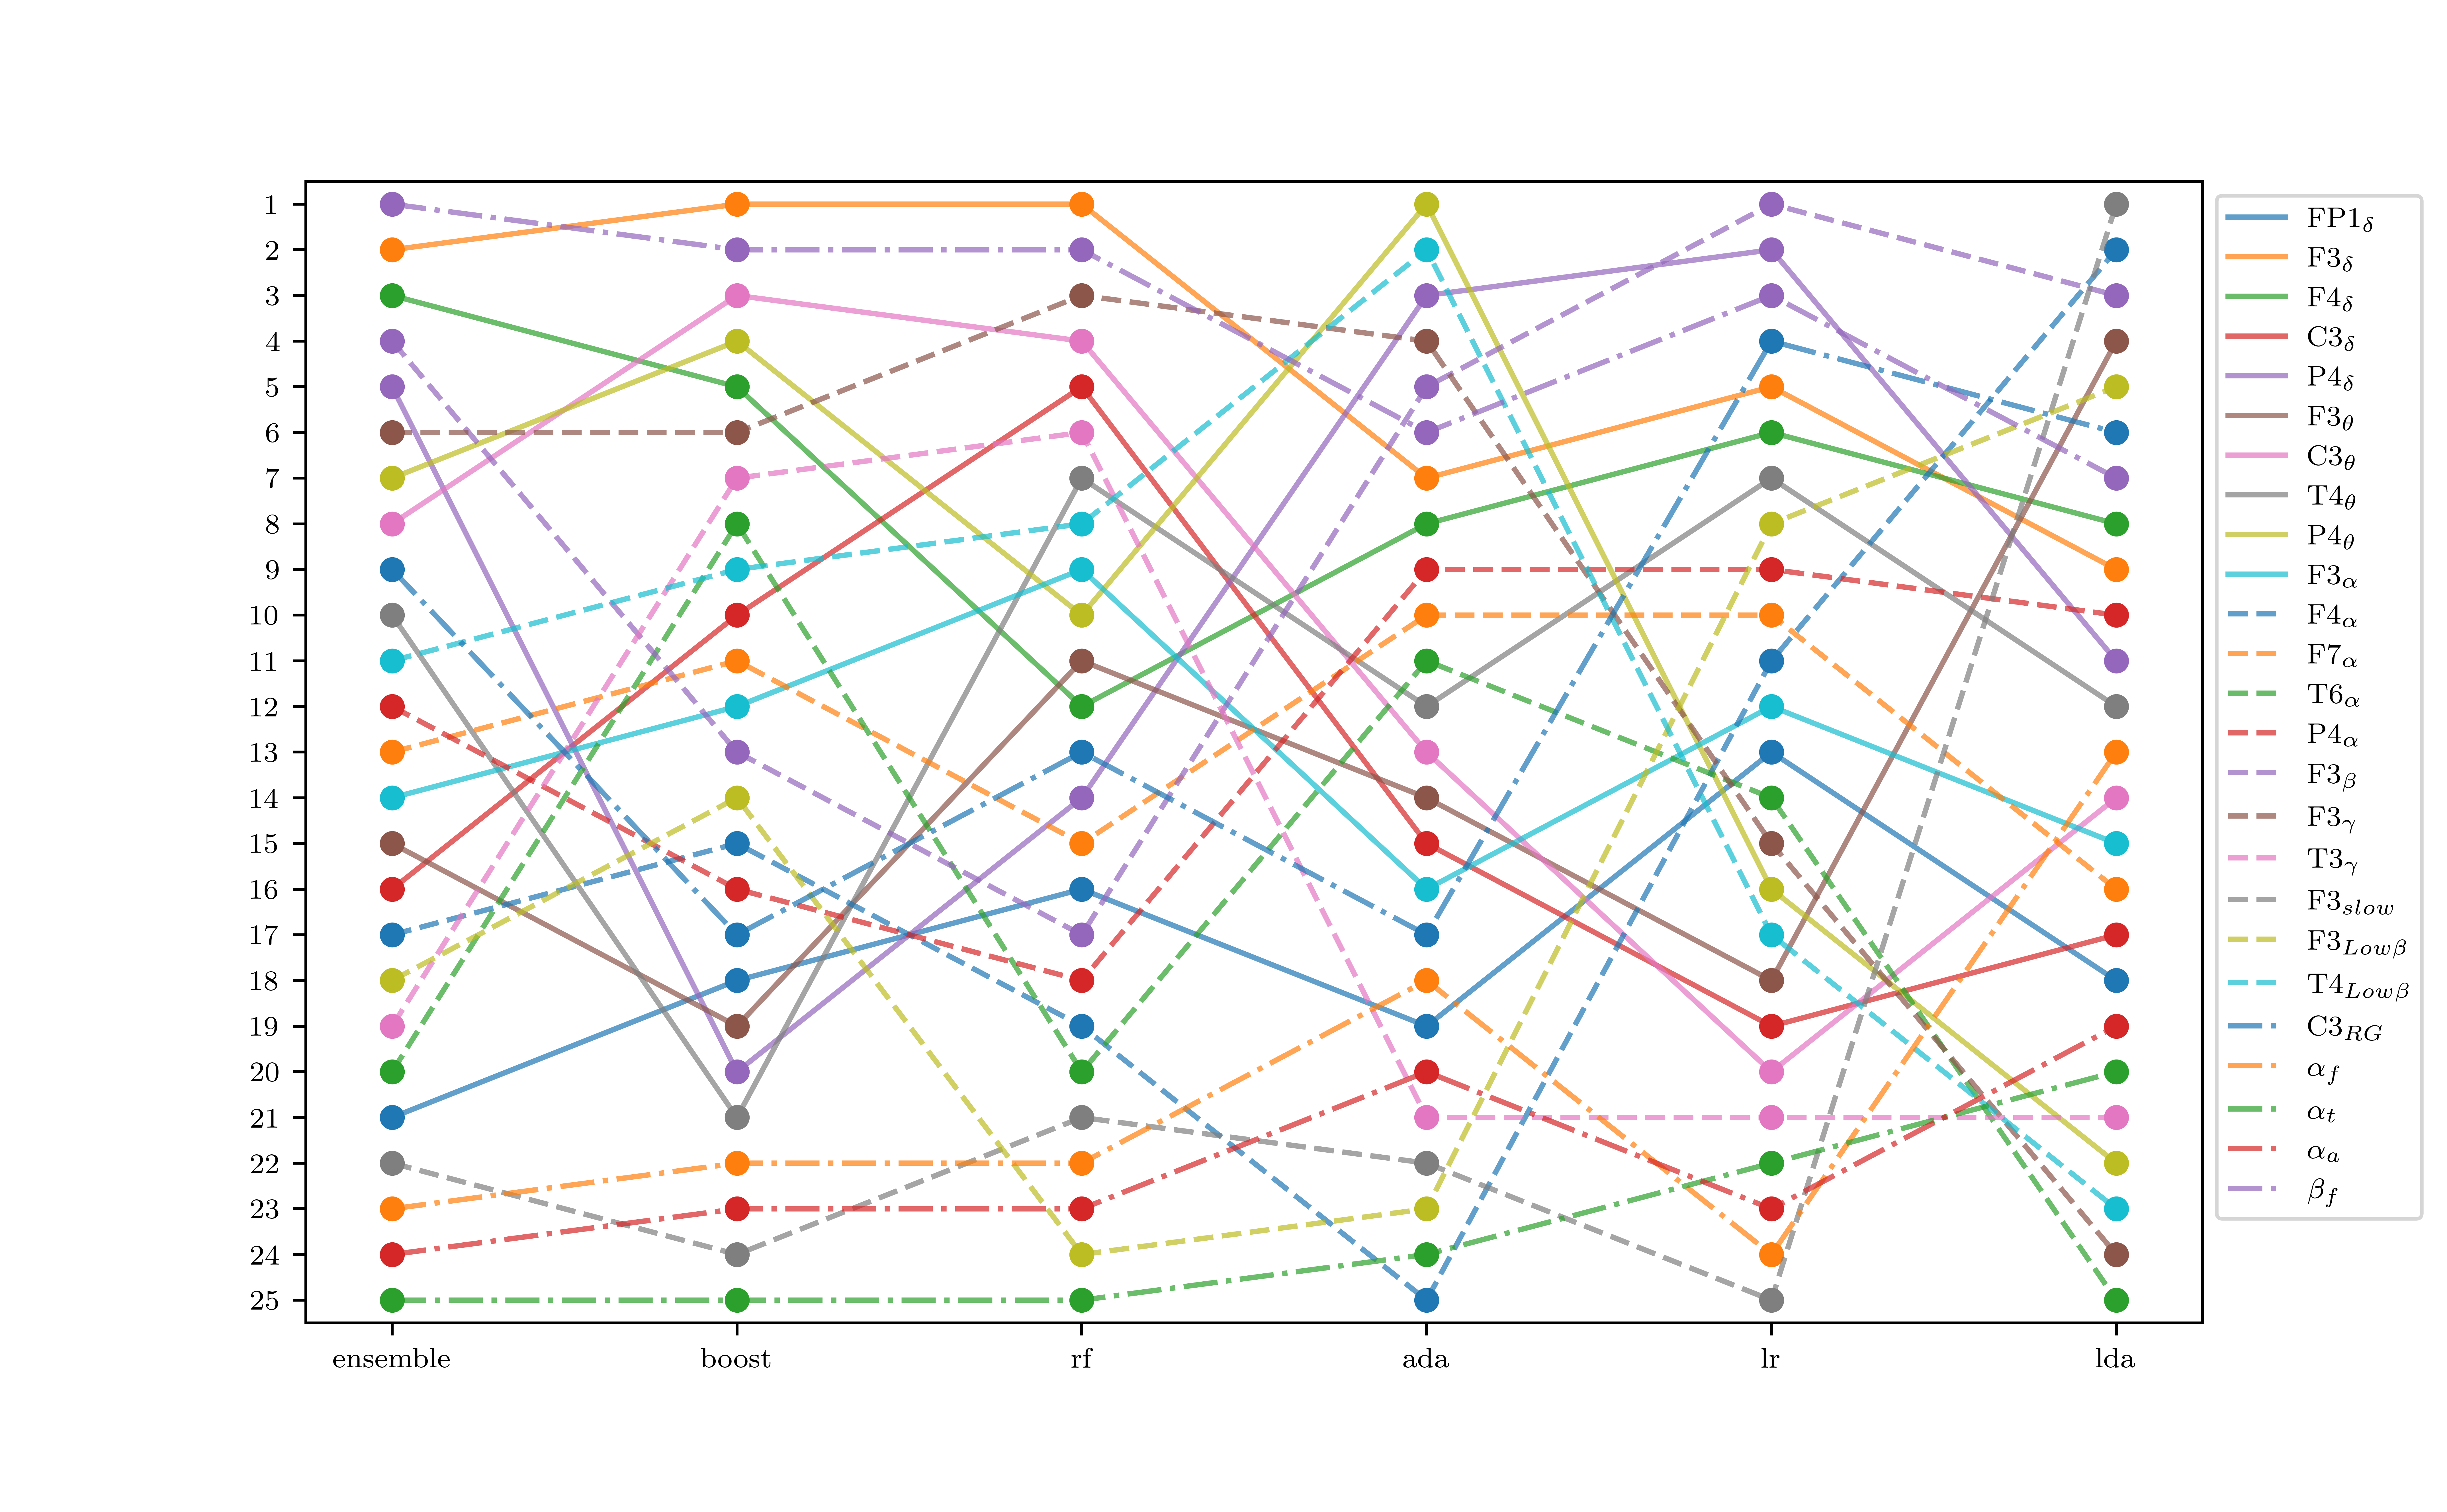
\includegraphics[width=1\textwidth]{figures/bump_chart.png}
  \label{fig:bump_chart}
\end{figure}




\begin{table}[h!]
\centering
\caption{The 10-CV score of each classifier when using $\text{Rank}_{\text{baseline}}$ as a rank.}
\label{tab:cv_baseline_apen}
\scalebox{0.72}{
\begin{tabular}{r|ccccccc}
\hline
 No. & $\text{Rank}_{\text{baseline}}$ &                      SVM &                       LR &                       GB &                      ADA &                       RF &                      LDA \\
\hline
   1 &           $\text{FP1}_{\delta}$ &          0.621$\pm$0.046 &          0.578$\pm$0.054 &          0.606$\pm$0.030 &          0.604$\pm$0.036 &          0.525$\pm$0.045 &          0.585$\pm$0.044 \\
   2 &            $\text{F3}_{\delta}$ &          0.740$\pm$0.061 &          0.678$\pm$0.055 &          0.733$\pm$0.047 &          0.710$\pm$0.049 &          0.724$\pm$0.061 &          0.676$\pm$0.045 \\
   3 &            $\text{F4}_{\delta}$ &          0.769$\pm$0.043 &          0.667$\pm$0.062 &          0.765$\pm$0.047 &          0.714$\pm$0.037 &          0.761$\pm$0.028 &          0.664$\pm$0.039 \\
   4 &            $\text{C3}_{\delta}$ &          0.829$\pm$0.044 &          0.678$\pm$0.077 &          0.832$\pm$0.038 &          0.761$\pm$0.036 &          0.843$\pm$0.028 &          0.675$\pm$0.043 \\
   5 &            $\text{P4}_{\delta}$ &          0.868$\pm$0.051 &          0.728$\pm$0.064 &          0.868$\pm$0.030 &          0.807$\pm$0.043 &          0.885$\pm$0.036 &          0.733$\pm$0.036 \\
   6 &            $\text{F3}_{\theta}$ &          0.875$\pm$0.041 &          0.722$\pm$0.049 &          0.853$\pm$0.050 &          0.821$\pm$0.074 &          0.878$\pm$0.058 &          0.724$\pm$0.055 \\
   7 &            $\text{C3}_{\theta}$ &          0.890$\pm$0.020 &          0.724$\pm$0.043 &          0.875$\pm$0.032 &          0.833$\pm$0.046 &          0.897$\pm$0.040 &          0.722$\pm$0.046 \\
   8 &            $\text{T4}_{\theta}$ & \textbf{0.915$\pm$0.031} &          0.764$\pm$0.033 &          0.883$\pm$0.052 &          0.843$\pm$0.030 & \textbf{0.907$\pm$0.030} &          0.751$\pm$0.054 \\
   9 &            $\text{P4}_{\theta}$ &          0.919$\pm$0.012 &          0.753$\pm$0.032 & \textbf{0.901$\pm$0.021} &          0.840$\pm$0.027 &          0.911$\pm$0.045 &          0.765$\pm$0.052 \\
  10 &            $\text{F3}_{\alpha}$ &          0.931$\pm$0.020 &          0.774$\pm$0.041 &          0.918$\pm$0.027 &          0.878$\pm$0.039 &          0.926$\pm$0.021 &          0.778$\pm$0.050 \\
  11 &            $\text{F4}_{\alpha}$ &          0.928$\pm$0.024 &          0.796$\pm$0.027 &          0.931$\pm$0.026 &          0.876$\pm$0.030 &          0.936$\pm$0.026 & \textbf{0.800$\pm$0.035} \\
  12 &            $\text{F7}_{\alpha}$ &          0.933$\pm$0.028 &          0.781$\pm$0.048 &          0.928$\pm$0.028 &          0.867$\pm$0.034 &          0.939$\pm$0.028 &          0.793$\pm$0.032 \\
  13 &            $\text{T6}_{\alpha}$ &          0.946$\pm$0.031 &          0.790$\pm$0.036 &          0.940$\pm$0.019 &          0.869$\pm$0.038 &          0.936$\pm$0.036 &          0.789$\pm$0.042 \\
  14 &            $\text{P4}_{\alpha}$ &          0.956$\pm$0.016 &          0.783$\pm$0.045 &          0.933$\pm$0.027 &          0.899$\pm$0.037 &          0.947$\pm$0.024 &          0.788$\pm$0.030 \\
  15 &             $\text{F3}_{\beta}$ &          0.961$\pm$0.023 &          0.788$\pm$0.041 &          0.940$\pm$0.028 &          0.882$\pm$0.041 &          0.957$\pm$0.020 &          0.769$\pm$0.033 \\
  16 &            $\text{F3}_{\gamma}$ &          0.978$\pm$0.015 & \textbf{0.815$\pm$0.037} &          0.951$\pm$0.022 & \textbf{0.924$\pm$0.029} &          0.969$\pm$0.022 &          0.814$\pm$0.032 \\
  17 &            $\text{T3}_{\gamma}$ &          0.976$\pm$0.023 &          0.811$\pm$0.044 &          0.956$\pm$0.030 &          0.912$\pm$0.027 &          0.975$\pm$0.015 &          0.814$\pm$0.044 \\
  18 &         $\text{F3}_\text{slow}$ &          0.974$\pm$0.015 &          0.808$\pm$0.040 &          0.961$\pm$0.025 &          0.914$\pm$0.031 &          0.968$\pm$0.024 &          0.817$\pm$0.047 \\
  19 &   $\text{F3}_{\text{Low}\beta}$ &          0.976$\pm$0.011 &          0.811$\pm$0.040 &          0.960$\pm$0.020 &          0.911$\pm$0.024 &          0.971$\pm$0.025 &          0.808$\pm$0.042 \\
  20 &   $\text{T4}_{\text{Low}\beta}$ &          0.982$\pm$0.014 &          0.825$\pm$0.058 &          0.958$\pm$0.012 &          0.918$\pm$0.027 &          0.974$\pm$0.013 &          0.812$\pm$0.051 \\
  21 &         $\text{C3}_{\text{RG}}$ &          0.981$\pm$0.013 &          0.838$\pm$0.022 &          0.958$\pm$0.020 &          0.904$\pm$0.021 &          0.971$\pm$0.018 &          0.814$\pm$0.043 \\
  22 &                    $\alpha_{f}$ &          0.979$\pm$0.007 &          0.824$\pm$0.041 &          0.962$\pm$0.015 &          0.912$\pm$0.036 &          0.975$\pm$0.020 &          0.819$\pm$0.041 \\
  23 &                    $\alpha_{t}$ &          0.981$\pm$0.009 &          0.833$\pm$0.037 &          0.964$\pm$0.015 &          0.924$\pm$0.032 &          0.969$\pm$0.021 &          0.821$\pm$0.042 \\
  24 &                    $\alpha_{a}$ &          0.978$\pm$0.013 &          0.838$\pm$0.031 &          0.968$\pm$0.022 &          0.914$\pm$0.037 &          0.979$\pm$0.016 &          0.826$\pm$0.031 \\
  25 &                     $\beta_{f}$ &          0.979$\pm$0.014 &          0.844$\pm$0.040 &          0.961$\pm$0.022 &          0.917$\pm$0.037 &          0.972$\pm$0.014 &          0.831$\pm$0.033 \\
\hline
\end{tabular}
}
\end{table}


\begin{table}[h!]
\centering
\caption{The 10-CV score of each classifier when using $\text{Rank}_{\text{LR}}$ as a rank.}
\label{tab:cv_lr_apen}
\scalebox{0.69}{
\begin{tabular}{r|cccccccc}
\hline
 No. &     $\text{Rank}_{\text{LR}}$ &  coeff &                      SVM &                       LR &                       GB &                      ADA &                       RF &                      LDA \\
\hline
   1 &           $\text{F3}_{\beta}$ &  1.894 &          0.575$\pm$0.051 &          0.558$\pm$0.040 &          0.561$\pm$0.072 &          0.607$\pm$0.075 &          0.564$\pm$0.057 &          0.565$\pm$0.046 \\
   2 &          $\text{P4}_{\delta}$ &  1.651 &          0.635$\pm$0.050 &          0.571$\pm$0.048 &          0.656$\pm$0.033 &          0.610$\pm$0.054 &          0.693$\pm$0.036 &          0.571$\pm$0.047 \\
   3 &                   $\beta_{f}$ & -1.435 &          0.749$\pm$0.058 &          0.624$\pm$0.051 &          0.753$\pm$0.047 &          0.742$\pm$0.039 &          0.814$\pm$0.055 &          0.624$\pm$0.054 \\
   4 &       $\text{C3}_{\text{RG}}$ & -1.346 &          0.858$\pm$0.034 &          0.646$\pm$0.032 &          0.856$\pm$0.032 &          0.781$\pm$0.034 &          0.885$\pm$0.035 &          0.647$\pm$0.044 \\
   5 &          $\text{F3}_{\delta}$ & -1.273 &          0.886$\pm$0.030 &          0.718$\pm$0.047 &          0.875$\pm$0.052 &          0.826$\pm$0.044 &          0.897$\pm$0.019 &          0.715$\pm$0.024 \\
   6 &          $\text{F4}_{\delta}$ & -1.258 & \textbf{0.900$\pm$0.042} &          0.735$\pm$0.061 &          0.899$\pm$0.028 &          0.850$\pm$0.035 & \textbf{0.912$\pm$0.028} &          0.749$\pm$0.015 \\
   7 &          $\text{T4}_{\theta}$ &  0.952 &          0.910$\pm$0.029 &          0.735$\pm$0.053 & \textbf{0.900$\pm$0.038} &          0.865$\pm$0.036 &          0.922$\pm$0.044 &          0.754$\pm$0.041 \\
   8 & $\text{F3}_{\text{Low}\beta}$ & -0.841 &          0.921$\pm$0.037 &          0.765$\pm$0.054 &          0.896$\pm$0.052 &          0.868$\pm$0.037 &          0.931$\pm$0.039 &          0.761$\pm$0.044 \\
   9 &          $\text{P4}_{\alpha}$ & -0.833 &          0.961$\pm$0.014 & \textbf{0.836$\pm$0.040} &          0.931$\pm$0.026 &          0.888$\pm$0.033 &          0.940$\pm$0.018 & \textbf{0.836$\pm$0.046} \\
  10 &          $\text{F7}_{\alpha}$ &  0.767 &          0.961$\pm$0.022 &          0.832$\pm$0.040 &          0.932$\pm$0.035 &          0.893$\pm$0.036 &          0.960$\pm$0.028 &          0.835$\pm$0.067 \\
  11 &          $\text{F4}_{\alpha}$ & -0.609 &          0.960$\pm$0.018 &          0.846$\pm$0.048 &          0.947$\pm$0.024 &          0.893$\pm$0.031 &          0.946$\pm$0.021 &          0.840$\pm$0.049 \\
  12 &          $\text{F3}_{\alpha}$ & -0.594 &          0.961$\pm$0.016 &          0.858$\pm$0.045 &          0.942$\pm$0.024 & \textbf{0.900$\pm$0.025} &          0.949$\pm$0.027 &          0.846$\pm$0.040 \\
  13 &         $\text{FP1}_{\delta}$ & -0.503 &          0.964$\pm$0.015 &          0.849$\pm$0.052 &          0.938$\pm$0.021 &          0.908$\pm$0.031 &          0.953$\pm$0.021 &          0.839$\pm$0.037 \\
  14 &          $\text{T6}_{\alpha}$ & -0.465 &          0.957$\pm$0.015 &          0.854$\pm$0.019 &          0.939$\pm$0.031 &          0.917$\pm$0.032 &          0.951$\pm$0.024 &          0.836$\pm$0.043 \\
  15 &          $\text{F3}_{\gamma}$ &  0.422 &          0.957$\pm$0.031 &          0.856$\pm$0.032 &          0.956$\pm$0.024 &          0.912$\pm$0.035 &          0.964$\pm$0.020 &          0.842$\pm$0.045 \\
  16 &          $\text{P4}_{\theta}$ &  0.405 &          0.971$\pm$0.018 &          0.851$\pm$0.049 &          0.951$\pm$0.027 &          0.935$\pm$0.026 &          0.967$\pm$0.017 &          0.846$\pm$0.024 \\
  17 & $\text{T4}_{\text{Low}\beta}$ &  0.396 &          0.968$\pm$0.019 &          0.850$\pm$0.041 &          0.961$\pm$0.010 &          0.922$\pm$0.036 &          0.968$\pm$0.028 &          0.839$\pm$0.048 \\
  18 &          $\text{F3}_{\theta}$ & -0.384 &          0.969$\pm$0.016 &          0.854$\pm$0.037 &          0.962$\pm$0.018 &          0.935$\pm$0.021 &          0.968$\pm$0.014 &          0.838$\pm$0.064 \\
  19 &          $\text{C3}_{\delta}$ &  0.350 &          0.982$\pm$0.013 &          0.846$\pm$0.036 &          0.962$\pm$0.021 &          0.938$\pm$0.027 &          0.972$\pm$0.021 &          0.843$\pm$0.033 \\
  20 &          $\text{C3}_{\theta}$ & -0.348 &          0.979$\pm$0.016 &          0.847$\pm$0.020 &          0.951$\pm$0.029 &          0.936$\pm$0.017 &          0.967$\pm$0.021 &          0.831$\pm$0.034 \\
  21 &          $\text{T3}_{\gamma}$ & -0.323 &          0.979$\pm$0.011 &          0.850$\pm$0.034 &          0.957$\pm$0.025 &          0.939$\pm$0.029 &          0.974$\pm$0.020 &          0.835$\pm$0.023 \\
  22 &                  $\alpha_{t}$ & -0.201 &          0.975$\pm$0.019 &          0.853$\pm$0.034 &          0.962$\pm$0.033 &          0.925$\pm$0.033 &          0.969$\pm$0.018 &          0.829$\pm$0.038 \\
  23 &                  $\alpha_{a}$ & -0.182 &          0.981$\pm$0.023 &          0.853$\pm$0.035 &          0.954$\pm$0.014 &          0.917$\pm$0.039 &          0.976$\pm$0.025 &          0.829$\pm$0.036 \\
  24 &                  $\alpha_{f}$ & -0.067 &          0.979$\pm$0.017 &          0.847$\pm$0.052 &          0.964$\pm$0.029 &          0.919$\pm$0.031 &          0.976$\pm$0.012 &          0.826$\pm$0.040 \\
  25 &       $\text{F3}_\text{slow}$ &  0.036 &          0.975$\pm$0.015 &          0.840$\pm$0.042 &          0.956$\pm$0.018 &          0.925$\pm$0.021 &          0.974$\pm$0.016 &          0.833$\pm$0.041 \\
\hline
\end{tabular}
}
\end{table}


\begin{table}[h!]
\centering
\caption{The 10-CV score of each classifier when using $\text{Rank}_{\text{LDA}}$ as a rank.}
\label{tab:cv_lda_apen}
\scalebox{0.68}{
\begin{tabular}{r|cccccccc}
\hline
 No. &    $\text{Rank}_{\text{LDA}}$ &  score &                      SVM &                       LR &                       GB &                      ADA &                       RF &                      LDA \\
\hline
   1 &       $\text{F3}_\text{slow}$ &  4.658 &          0.603$\pm$0.044 &          0.589$\pm$0.046 &          0.593$\pm$0.052 &          0.592$\pm$0.059 &          0.610$\pm$0.055 &          0.583$\pm$0.043 \\
   2 &          $\text{F4}_{\alpha}$ & -3.383 &          0.707$\pm$0.040 &          0.640$\pm$0.055 &          0.703$\pm$0.063 &          0.682$\pm$0.050 &          0.706$\pm$0.053 &          0.643$\pm$0.058 \\
   3 &           $\text{F3}_{\beta}$ &  3.258 &          0.726$\pm$0.038 &          0.658$\pm$0.049 &          0.758$\pm$0.051 &          0.718$\pm$0.046 &          0.783$\pm$0.038 &          0.650$\pm$0.064 \\
   4 &          $\text{F3}_{\theta}$ & -2.143 &          0.749$\pm$0.049 &          0.633$\pm$0.039 &          0.800$\pm$0.024 &          0.729$\pm$0.053 &          0.818$\pm$0.043 &          0.629$\pm$0.041 \\
   5 & $\text{F3}_{\text{Low}\beta}$ & -1.710 &          0.753$\pm$0.046 &          0.651$\pm$0.044 &          0.788$\pm$0.032 &          0.775$\pm$0.041 &          0.804$\pm$0.049 &          0.649$\pm$0.066 \\
   6 &       $\text{C3}_{\text{RG}}$ & -1.595 &          0.800$\pm$0.042 &          0.679$\pm$0.049 &          0.808$\pm$0.044 &          0.738$\pm$0.045 &          0.847$\pm$0.041 &          0.674$\pm$0.044 \\
   7 &                   $\beta_{f}$ & -1.398 &          0.854$\pm$0.049 &          0.707$\pm$0.041 &          0.882$\pm$0.027 &          0.824$\pm$0.025 &          0.886$\pm$0.038 &          0.725$\pm$0.043 \\
   8 &          $\text{F4}_{\delta}$ & -1.289 &          0.883$\pm$0.048 &          0.714$\pm$0.053 &          0.886$\pm$0.044 &          0.856$\pm$0.037 & \textbf{0.917$\pm$0.026} &          0.725$\pm$0.026 \\
   9 &          $\text{F3}_{\delta}$ & -1.227 &          0.897$\pm$0.031 &          0.767$\pm$0.057 &          0.893$\pm$0.030 &          0.868$\pm$0.023 &          0.912$\pm$0.041 &          0.782$\pm$0.026 \\
  10 &          $\text{P4}_{\alpha}$ & -1.155 & \textbf{0.911$\pm$0.022} &          0.783$\pm$0.042 & \textbf{0.910$\pm$0.030} &          0.867$\pm$0.050 &          0.918$\pm$0.040 &          0.785$\pm$0.058 \\
  11 &          $\text{P4}_{\delta}$ &  1.143 &          0.958$\pm$0.022 & \textbf{0.828$\pm$0.039} &          0.925$\pm$0.030 &          0.892$\pm$0.036 &          0.944$\pm$0.022 & \textbf{0.832$\pm$0.034} \\
  12 &          $\text{T4}_{\theta}$ &  1.069 &          0.960$\pm$0.027 &          0.849$\pm$0.037 &          0.947$\pm$0.022 &          0.899$\pm$0.035 &          0.954$\pm$0.022 &          0.844$\pm$0.044 \\
  13 &                  $\alpha_{f}$ & -1.042 &          0.957$\pm$0.027 &          0.850$\pm$0.029 &          0.942$\pm$0.019 & \textbf{0.906$\pm$0.037} &          0.953$\pm$0.026 &          0.844$\pm$0.046 \\
  14 &          $\text{C3}_{\theta}$ & -0.639 &          0.972$\pm$0.020 &          0.850$\pm$0.048 &          0.943$\pm$0.027 &          0.915$\pm$0.024 &          0.967$\pm$0.021 &          0.838$\pm$0.044 \\
  15 &          $\text{F3}_{\alpha}$ & -0.458 &          0.975$\pm$0.021 &          0.847$\pm$0.033 &          0.944$\pm$0.029 &          0.914$\pm$0.044 &          0.960$\pm$0.018 &          0.839$\pm$0.034 \\
  16 &          $\text{F7}_{\alpha}$ &  0.395 &          0.976$\pm$0.014 &          0.851$\pm$0.042 &          0.946$\pm$0.031 &          0.914$\pm$0.030 &          0.961$\pm$0.023 &          0.835$\pm$0.032 \\
  17 &          $\text{C3}_{\delta}$ &  0.364 &          0.972$\pm$0.022 &          0.851$\pm$0.045 &          0.946$\pm$0.025 &          0.919$\pm$0.028 &          0.968$\pm$0.020 &          0.833$\pm$0.024 \\
  18 &         $\text{FP1}_{\delta}$ & -0.339 &          0.975$\pm$0.016 &          0.850$\pm$0.038 &          0.950$\pm$0.039 &          0.890$\pm$0.031 &          0.960$\pm$0.023 &          0.832$\pm$0.038 \\
  19 &                  $\alpha_{a}$ & -0.279 &          0.979$\pm$0.019 &          0.839$\pm$0.044 &          0.946$\pm$0.023 &          0.915$\pm$0.031 &          0.961$\pm$0.025 &          0.835$\pm$0.036 \\
  20 &                  $\alpha_{t}$ &  0.271 &          0.974$\pm$0.025 &          0.847$\pm$0.025 &          0.953$\pm$0.029 &          0.912$\pm$0.028 &          0.972$\pm$0.015 &          0.836$\pm$0.043 \\
  21 &          $\text{T3}_{\gamma}$ &  0.180 &          0.978$\pm$0.019 &          0.849$\pm$0.034 &          0.953$\pm$0.020 &          0.904$\pm$0.029 &          0.974$\pm$0.021 &          0.835$\pm$0.040 \\
  22 &          $\text{P4}_{\theta}$ &  0.077 &          0.974$\pm$0.015 &          0.849$\pm$0.034 &          0.947$\pm$0.039 &          0.910$\pm$0.044 &          0.968$\pm$0.018 &          0.838$\pm$0.044 \\
  23 & $\text{T4}_{\text{Low}\beta}$ &  0.066 &          0.979$\pm$0.017 &          0.849$\pm$0.024 &          0.953$\pm$0.026 &          0.911$\pm$0.032 &          0.978$\pm$0.015 &          0.825$\pm$0.053 \\
  24 &          $\text{F3}_{\gamma}$ & -0.042 &          0.978$\pm$0.015 &          0.842$\pm$0.042 &          0.964$\pm$0.029 &          0.925$\pm$0.038 &          0.971$\pm$0.034 &          0.832$\pm$0.033 \\
  25 &          $\text{T6}_{\alpha}$ &  0.022 &          0.976$\pm$0.013 &          0.847$\pm$0.037 &          0.962$\pm$0.019 &          0.932$\pm$0.027 &          0.975$\pm$0.023 &          0.835$\pm$0.051 \\
\hline
\end{tabular}
}
\end{table}

% ada

\begin{table}[h!]
\centering
\caption{The 10-CV score of each classifier when using $\text{Rank}_{\text{ADA}}$ as a rank.}
\label{tab:cv_ada_apen}
\scalebox{0.69}{
\begin{tabular}{r|cccccccc}
\hline
 No. &    $\text{Rank}_{\text{ADA}}$ &  score &                      SVM &                       LR &                       GB &                      ADA &                       RF &                      LDA \\
\hline
   1 &          $\text{P4}_{\theta}$ &   0.10 &          0.594$\pm$0.070 &          0.538$\pm$0.026 &          0.571$\pm$0.040 &          0.604$\pm$0.044 &          0.517$\pm$0.071 &          0.539$\pm$0.032 \\
   2 & $\text{T4}_{\text{Low}\beta}$ &   0.08 &          0.703$\pm$0.041 &          0.572$\pm$0.045 &          0.656$\pm$0.065 &          0.633$\pm$0.029 &          0.636$\pm$0.054 &          0.569$\pm$0.031 \\
   3 &          $\text{P4}_{\delta}$ &   0.08 &          0.742$\pm$0.042 &          0.604$\pm$0.035 &          0.731$\pm$0.032 &          0.682$\pm$0.052 &          0.750$\pm$0.046 &          0.599$\pm$0.052 \\
   4 &          $\text{F3}_{\gamma}$ &   0.08 &          0.835$\pm$0.026 &          0.610$\pm$0.051 &          0.879$\pm$0.028 &          0.774$\pm$0.054 &          0.893$\pm$0.027 &          0.612$\pm$0.047 \\
   5 &           $\text{F3}_{\beta}$ &   0.08 &          0.853$\pm$0.026 &          0.633$\pm$0.055 &          0.899$\pm$0.038 &          0.794$\pm$0.037 & \textbf{0.915$\pm$0.038} &          0.621$\pm$0.041 \\
   6 &                   $\beta_{f}$ &   0.08 &          0.893$\pm$0.030 &          0.678$\pm$0.050 & \textbf{0.924$\pm$0.033} &          0.846$\pm$0.055 &          0.940$\pm$0.029 &          0.676$\pm$0.048 \\
   7 &          $\text{F3}_{\delta}$ &   0.06 & \textbf{0.921$\pm$0.033} &          0.733$\pm$0.044 &          0.942$\pm$0.040 & \textbf{0.906$\pm$0.029} &          0.958$\pm$0.024 &          0.739$\pm$0.054 \\
   8 &          $\text{F4}_{\delta}$ &   0.06 &          0.932$\pm$0.037 &          0.756$\pm$0.035 &          0.947$\pm$0.019 &          0.901$\pm$0.027 &          0.961$\pm$0.014 &          0.769$\pm$0.052 \\
   9 &          $\text{P4}_{\alpha}$ &   0.06 &          0.949$\pm$0.028 & \textbf{0.800$\pm$0.049} &          0.942$\pm$0.038 &          0.917$\pm$0.024 &          0.964$\pm$0.021 & \textbf{0.804$\pm$0.054} \\
  10 &          $\text{F7}_{\alpha}$ &   0.06 &          0.954$\pm$0.021 &          0.807$\pm$0.048 &          0.950$\pm$0.025 &          0.932$\pm$0.023 &          0.964$\pm$0.028 &          0.803$\pm$0.054 \\
  11 &          $\text{T6}_{\alpha}$ &   0.04 &          0.958$\pm$0.022 &          0.811$\pm$0.038 &          0.962$\pm$0.022 &          0.921$\pm$0.028 &          0.968$\pm$0.016 &          0.806$\pm$0.039 \\
  12 &          $\text{T4}_{\theta}$ &   0.04 &          0.964$\pm$0.023 &          0.828$\pm$0.049 &          0.965$\pm$0.025 &          0.928$\pm$0.030 &          0.975$\pm$0.017 &          0.810$\pm$0.038 \\
  13 &          $\text{C3}_{\theta}$ &   0.04 &          0.976$\pm$0.022 &          0.821$\pm$0.031 &          0.957$\pm$0.025 &          0.926$\pm$0.028 &          0.969$\pm$0.014 &          0.819$\pm$0.043 \\
  14 &          $\text{F3}_{\theta}$ &   0.04 &          0.979$\pm$0.023 &          0.821$\pm$0.058 &          0.954$\pm$0.028 &          0.933$\pm$0.038 &          0.972$\pm$0.026 &          0.817$\pm$0.047 \\
  15 &          $\text{C3}_{\delta}$ &   0.02 &          0.981$\pm$0.017 &          0.821$\pm$0.048 &          0.964$\pm$0.018 &          0.944$\pm$0.022 &          0.969$\pm$0.016 &          0.825$\pm$0.049 \\
  16 &          $\text{F3}_{\alpha}$ &   0.02 &          0.979$\pm$0.025 &          0.832$\pm$0.045 &          0.956$\pm$0.008 &          0.924$\pm$0.035 &          0.975$\pm$0.023 &          0.833$\pm$0.037 \\
  17 &       $\text{C3}_{\text{RG}}$ &   0.02 &          0.978$\pm$0.023 &          0.846$\pm$0.040 &          0.967$\pm$0.019 &          0.935$\pm$0.015 &          0.975$\pm$0.018 &          0.828$\pm$0.030 \\
  18 &                  $\alpha_{f}$ &   0.02 &          0.979$\pm$0.014 &          0.847$\pm$0.049 &          0.957$\pm$0.020 &          0.936$\pm$0.021 &          0.976$\pm$0.022 &          0.825$\pm$0.029 \\
  19 &         $\text{FP1}_{\delta}$ &   0.02 &          0.979$\pm$0.022 &          0.843$\pm$0.044 &          0.960$\pm$0.013 &          0.929$\pm$0.030 &          0.972$\pm$0.023 &          0.826$\pm$0.034 \\
  20 &                  $\alpha_{a}$ &   0.00 &          0.981$\pm$0.020 &          0.846$\pm$0.051 &          0.964$\pm$0.021 &          0.929$\pm$0.020 &          0.975$\pm$0.016 &          0.817$\pm$0.043 \\
  21 &          $\text{T3}_{\gamma}$ &   0.00 &          0.982$\pm$0.006 &          0.843$\pm$0.034 &          0.963$\pm$0.022 &          0.928$\pm$0.040 &          0.978$\pm$0.017 &          0.826$\pm$0.046 \\
  22 &       $\text{F3}_\text{slow}$ &   0.00 &          0.981$\pm$0.017 &          0.839$\pm$0.057 &          0.967$\pm$0.023 &          0.924$\pm$0.027 &          0.981$\pm$0.021 &          0.829$\pm$0.054 \\
  23 & $\text{F3}_{\text{Low}\beta}$ &   0.00 &          0.982$\pm$0.013 &          0.843$\pm$0.036 &          0.968$\pm$0.015 &          0.914$\pm$0.033 &          0.979$\pm$0.014 &          0.832$\pm$0.037 \\
  24 &                  $\alpha_{t}$ &   0.00 &          0.975$\pm$0.021 &          0.847$\pm$0.023 &          0.958$\pm$0.032 &          0.918$\pm$0.018 &          0.983$\pm$0.015 &          0.832$\pm$0.015 \\
  25 &          $\text{F4}_{\alpha}$ &   0.00 &          0.975$\pm$0.016 &          0.847$\pm$0.022 &          0.956$\pm$0.026 &          0.906$\pm$0.043 &          0.972$\pm$0.020 &          0.831$\pm$0.037 \\
\hline
\end{tabular}
}
\end{table}


% gb

\begin{table}[h!]
\centering
\caption{The 10-CV score of each classifier when using $\text{Rank}_{\text{GB}}$ as a rank.}
\label{tab:cv_gb_apen}
\scalebox{0.69}{
\begin{tabular}{r|cccccccc}
\hline
 No. &     $\text{Rank}_{\text{GB}}$ &  score &                      SVM &                       LR &                       GB &                      ADA &                       RF &                      LDA \\
\hline
   1 &          $\text{F3}_{\delta}$ &  0.140 &          0.679$\pm$0.049 &          0.689$\pm$0.041 &          0.668$\pm$0.051 &          0.688$\pm$0.047 &          0.582$\pm$0.053 &          0.688$\pm$0.024 \\
   2 &                   $\beta_{f}$ &  0.099 &          0.767$\pm$0.024 &          0.731$\pm$0.050 &          0.761$\pm$0.040 &          0.749$\pm$0.042 &          0.732$\pm$0.049 &          0.725$\pm$0.054 \\
   3 &          $\text{C3}_{\theta}$ &  0.082 &          0.810$\pm$0.039 &          0.718$\pm$0.031 &          0.782$\pm$0.050 &          0.806$\pm$0.033 &          0.803$\pm$0.032 &          0.714$\pm$0.042 \\
   4 &          $\text{P4}_{\theta}$ &  0.076 &          0.836$\pm$0.025 &          0.704$\pm$0.040 &          0.822$\pm$0.024 &          0.831$\pm$0.037 &          0.846$\pm$0.036 &          0.707$\pm$0.047 \\
   5 &          $\text{F4}_{\delta}$ &  0.073 &          0.858$\pm$0.015 &          0.721$\pm$0.054 &          0.851$\pm$0.034 &          0.836$\pm$0.031 &          0.868$\pm$0.025 &          0.721$\pm$0.035 \\
   6 &          $\text{F3}_{\gamma}$ &  0.071 &          0.894$\pm$0.034 &          0.719$\pm$0.049 & \textbf{0.919$\pm$0.037} &          0.894$\pm$0.029 & \textbf{0.936$\pm$0.021} &          0.722$\pm$0.046 \\
   7 &          $\text{T3}_{\gamma}$ &  0.069 & \textbf{0.917$\pm$0.030} &          0.732$\pm$0.049 &          0.932$\pm$0.042 &          0.892$\pm$0.037 &          0.953$\pm$0.022 &          0.735$\pm$0.039 \\
   8 &          $\text{T6}_{\alpha}$ &  0.061 &          0.950$\pm$0.026 &          0.740$\pm$0.063 &          0.933$\pm$0.031 & \textbf{0.910$\pm$0.029} &          0.956$\pm$0.028 &          0.740$\pm$0.072 \\
   9 & $\text{T4}_{\text{Low}\beta}$ &  0.050 &          0.957$\pm$0.021 &          0.778$\pm$0.060 &          0.953$\pm$0.027 &          0.922$\pm$0.028 &          0.956$\pm$0.023 &          0.776$\pm$0.035 \\
  10 &          $\text{C3}_{\delta}$ &  0.040 &          0.953$\pm$0.015 &          0.776$\pm$0.053 &          0.947$\pm$0.036 &          0.897$\pm$0.020 &          0.954$\pm$0.022 &          0.776$\pm$0.040 \\
  11 &          $\text{F7}_{\alpha}$ &  0.036 &          0.960$\pm$0.018 &          0.772$\pm$0.059 &          0.956$\pm$0.023 &          0.919$\pm$0.025 &          0.971$\pm$0.020 &          0.781$\pm$0.034 \\
  12 &          $\text{F3}_{\alpha}$ &  0.034 &          0.957$\pm$0.024 &          0.771$\pm$0.063 &          0.947$\pm$0.037 &          0.915$\pm$0.029 &          0.968$\pm$0.015 &          0.788$\pm$0.051 \\
  13 &           $\text{F3}_{\beta}$ &  0.026 &          0.972$\pm$0.019 &          0.779$\pm$0.036 &          0.949$\pm$0.029 &          0.931$\pm$0.019 &          0.976$\pm$0.021 & \textbf{0.801$\pm$0.056} \\
  14 & $\text{F3}_{\text{Low}\beta}$ &  0.021 &          0.974$\pm$0.021 &          0.789$\pm$0.043 &          0.953$\pm$0.011 &          0.921$\pm$0.027 &          0.974$\pm$0.015 &          0.817$\pm$0.031 \\
  15 &          $\text{F4}_{\alpha}$ &  0.016 &          0.972$\pm$0.024 &          0.797$\pm$0.049 &          0.956$\pm$0.022 &          0.922$\pm$0.032 &          0.972$\pm$0.021 &          0.822$\pm$0.025 \\
  16 &          $\text{P4}_{\alpha}$ &  0.015 &          0.975$\pm$0.014 & \textbf{0.801$\pm$0.030} &          0.961$\pm$0.017 &          0.938$\pm$0.034 &          0.974$\pm$0.024 &          0.804$\pm$0.048 \\
  17 &       $\text{C3}_{\text{RG}}$ &  0.014 &          0.976$\pm$0.016 &          0.826$\pm$0.036 &          0.957$\pm$0.024 &          0.925$\pm$0.029 &          0.971$\pm$0.013 &          0.817$\pm$0.028 \\
  18 &         $\text{FP1}_{\delta}$ &  0.014 &          0.972$\pm$0.014 &          0.822$\pm$0.051 &          0.957$\pm$0.030 &          0.929$\pm$0.031 &          0.967$\pm$0.014 &          0.808$\pm$0.043 \\
  19 &          $\text{F3}_{\theta}$ &  0.013 &          0.978$\pm$0.013 &          0.824$\pm$0.047 &          0.957$\pm$0.021 &          0.922$\pm$0.029 &          0.972$\pm$0.024 &          0.812$\pm$0.043 \\
  20 &          $\text{P4}_{\delta}$ &  0.012 &          0.981$\pm$0.013 &          0.839$\pm$0.029 &          0.960$\pm$0.020 &          0.921$\pm$0.032 &          0.975$\pm$0.015 &          0.826$\pm$0.044 \\
  21 &          $\text{T4}_{\theta}$ &  0.011 &          0.979$\pm$0.019 &          0.853$\pm$0.040 &          0.961$\pm$0.025 &          0.932$\pm$0.046 &          0.982$\pm$0.015 &          0.832$\pm$0.057 \\
  22 &                  $\alpha_{f}$ &  0.010 &          0.983$\pm$0.018 &          0.849$\pm$0.042 &          0.958$\pm$0.016 &          0.926$\pm$0.015 &          0.975$\pm$0.015 &          0.828$\pm$0.037 \\
  23 &                  $\alpha_{a}$ &  0.007 &          0.979$\pm$0.017 &          0.847$\pm$0.043 &          0.954$\pm$0.023 &          0.921$\pm$0.033 &          0.976$\pm$0.018 &          0.835$\pm$0.038 \\
  24 &       $\text{F3}_\text{slow}$ &  0.006 &          0.979$\pm$0.017 &          0.851$\pm$0.038 &          0.967$\pm$0.017 &          0.922$\pm$0.033 &          0.978$\pm$0.019 &          0.833$\pm$0.061 \\
  25 &                  $\alpha_{t}$ &  0.002 &          0.981$\pm$0.013 &          0.853$\pm$0.037 &          0.964$\pm$0.017 &          0.910$\pm$0.026 &          0.986$\pm$0.012 &          0.828$\pm$0.043 \\
\hline
\end{tabular}
}
\end{table}

% rf

\begin{table}[h!]
\centering
\caption{The 10-CV score of each classifier when using $\text{Rank}_{\text{RF}}$ as a rank.}
\label{tab:cv_rf_apen}
\scalebox{0.69}{
\begin{tabular}{r|cccccccc}
\hline
 No. &     $\text{Rank}_{\text{RF}}$ &  score &                      SVM &                       LR &                       GB &                      ADA &                       RF &                      LDA \\
\hline
   1 &          $\text{F3}_{\delta}$ &  0.103 &          0.686$\pm$0.068 &          0.693$\pm$0.033 &          0.669$\pm$0.048 &          0.694$\pm$0.026 &          0.568$\pm$0.070 &          0.690$\pm$0.039 \\
   2 &                   $\beta_{f}$ &  0.076 &          0.767$\pm$0.046 &          0.732$\pm$0.039 &          0.751$\pm$0.037 &          0.747$\pm$0.056 &          0.733$\pm$0.037 &          0.725$\pm$0.044 \\
   3 &          $\text{F3}_{\gamma}$ &  0.066 &          0.804$\pm$0.033 &          0.729$\pm$0.057 &          0.868$\pm$0.037 &          0.821$\pm$0.039 &          0.883$\pm$0.024 &          0.725$\pm$0.051 \\
   4 &          $\text{C3}_{\theta}$ &  0.052 &          0.847$\pm$0.038 &          0.701$\pm$0.067 &          0.879$\pm$0.043 &          0.864$\pm$0.050 &          0.885$\pm$0.029 &          0.711$\pm$0.058 \\
   5 &          $\text{C3}_{\delta}$ &  0.048 &          0.826$\pm$0.038 &          0.719$\pm$0.048 &          0.897$\pm$0.021 &          0.853$\pm$0.032 & \textbf{0.907$\pm$0.027} &          0.721$\pm$0.050 \\
   6 &          $\text{T3}_{\gamma}$ &  0.045 &          0.860$\pm$0.037 &          0.724$\pm$0.043 & \textbf{0.904$\pm$0.038} &          0.865$\pm$0.037 &          0.925$\pm$0.024 &          0.722$\pm$0.045 \\
   7 &          $\text{T4}_{\theta}$ &  0.045 &          0.872$\pm$0.025 &          0.717$\pm$0.031 &          0.914$\pm$0.034 &          0.868$\pm$0.039 &          0.950$\pm$0.023 &          0.726$\pm$0.040 \\
   8 & $\text{T4}_{\text{Low}\beta}$ &  0.045 &          0.890$\pm$0.043 &          0.731$\pm$0.057 &          0.919$\pm$0.025 &          0.894$\pm$0.031 &          0.957$\pm$0.017 &          0.742$\pm$0.041 \\
   9 &          $\text{F3}_{\alpha}$ &  0.041 & \textbf{0.917$\pm$0.030} &          0.776$\pm$0.039 &          0.925$\pm$0.023 &          0.896$\pm$0.025 &          0.951$\pm$0.042 &          0.785$\pm$0.034 \\
  10 &          $\text{P4}_{\theta}$ &  0.038 &          0.949$\pm$0.025 &          0.778$\pm$0.025 &          0.936$\pm$0.023 & \textbf{0.901$\pm$0.031} &          0.968$\pm$0.015 &          0.788$\pm$0.071 \\
  11 &          $\text{F3}_{\theta}$ &  0.038 &          0.944$\pm$0.019 &          0.774$\pm$0.033 &          0.935$\pm$0.030 &          0.901$\pm$0.032 &          0.975$\pm$0.016 &          0.786$\pm$0.038 \\
  12 &          $\text{F4}_{\delta}$ &  0.036 &          0.965$\pm$0.023 &          0.799$\pm$0.037 &          0.951$\pm$0.026 &          0.915$\pm$0.039 &          0.971$\pm$0.021 & \textbf{0.819$\pm$0.040} \\
  13 &       $\text{C3}_{\text{RG}}$ &  0.036 &          0.969$\pm$0.026 & \textbf{0.810$\pm$0.038} &          0.954$\pm$0.021 &          0.921$\pm$0.032 &          0.958$\pm$0.014 &          0.806$\pm$0.040 \\
  14 &          $\text{P4}_{\delta}$ &  0.036 &          0.969$\pm$0.018 &          0.833$\pm$0.059 &          0.960$\pm$0.019 &          0.919$\pm$0.022 &          0.971$\pm$0.024 &          0.822$\pm$0.026 \\
  15 &          $\text{F7}_{\alpha}$ &  0.035 &          0.975$\pm$0.018 &          0.836$\pm$0.037 &          0.957$\pm$0.024 &          0.907$\pm$0.022 &          0.974$\pm$0.023 &          0.828$\pm$0.028 \\
  16 &         $\text{FP1}_{\delta}$ &  0.033 &          0.978$\pm$0.015 &          0.847$\pm$0.038 &          0.953$\pm$0.023 &          0.912$\pm$0.036 &          0.974$\pm$0.013 &          0.825$\pm$0.025 \\
  17 &           $\text{F3}_{\beta}$ &  0.032 &          0.978$\pm$0.011 &          0.846$\pm$0.042 &          0.958$\pm$0.021 &          0.924$\pm$0.027 &          0.969$\pm$0.020 &          0.828$\pm$0.026 \\
  18 &          $\text{P4}_{\alpha}$ &  0.032 &          0.976$\pm$0.015 &          0.843$\pm$0.033 &          0.967$\pm$0.019 &          0.925$\pm$0.017 &          0.972$\pm$0.022 &          0.829$\pm$0.032 \\
  19 &          $\text{F4}_{\alpha}$ &  0.029 &          0.981$\pm$0.020 &          0.839$\pm$0.035 &          0.956$\pm$0.016 &          0.915$\pm$0.042 &          0.972$\pm$0.015 &          0.829$\pm$0.035 \\
  20 &          $\text{T6}_{\alpha}$ &  0.029 &          0.979$\pm$0.019 &          0.844$\pm$0.028 &          0.957$\pm$0.022 &          0.935$\pm$0.016 &          0.976$\pm$0.026 &          0.831$\pm$0.040 \\
  21 &       $\text{F3}_\text{slow}$ &  0.027 &          0.979$\pm$0.014 &          0.844$\pm$0.039 &          0.969$\pm$0.025 &          0.933$\pm$0.023 &          0.975$\pm$0.016 &          0.825$\pm$0.040 \\
  22 &                  $\alpha_{f}$ &  0.026 &          0.979$\pm$0.024 &          0.843$\pm$0.022 &          0.958$\pm$0.012 &          0.931$\pm$0.024 &          0.982$\pm$0.013 &          0.825$\pm$0.029 \\
  23 &                  $\alpha_{a}$ &  0.023 &          0.981$\pm$0.015 &          0.847$\pm$0.036 &          0.962$\pm$0.023 &          0.911$\pm$0.029 &          0.975$\pm$0.016 &          0.822$\pm$0.034 \\
  24 & $\text{F3}_{\text{Low}\beta}$ &  0.019 &          0.979$\pm$0.017 &          0.844$\pm$0.045 &          0.958$\pm$0.028 &          0.917$\pm$0.022 &          0.969$\pm$0.017 &          0.833$\pm$0.060 \\
  25 &                  $\alpha_{t}$ &  0.012 &          0.975$\pm$0.014 &          0.851$\pm$0.037 &          0.957$\pm$0.037 &          0.907$\pm$0.044 &          0.978$\pm$0.009 &          0.831$\pm$0.040 \\
\hline
\end{tabular}
}
\end{table}

\begin{table}[h!]
\centering
\caption{The 10-CV score of each classifier when using $\text{Rank}_{\text{Ensemble}}$ as a rank.}
\label{tab:cv_ensemble_apen}
\scalebox{0.67}{
\begin{tabular}{r|cccccccc}
\hline
 No. & $\text{Rank}_{\text{Ensemble}}$ &  score &                      SVM &                       LR &                       GB &                      ADA &                       RF &                      LDA \\
\hline
   1 &                     $\beta_{f}$ &     15 &          0.693$\pm$0.057 &          0.669$\pm$0.046 &          0.646$\pm$0.038 &          0.671$\pm$0.035 &          0.585$\pm$0.042 &          0.667$\pm$0.042 \\
   2 &            $\text{F3}_{\delta}$ &     18 &          0.765$\pm$0.029 &          0.731$\pm$0.048 &          0.742$\pm$0.050 &          0.736$\pm$0.043 &          0.733$\pm$0.036 &          0.728$\pm$0.038 \\
   3 &            $\text{F4}_{\delta}$ &     34 &          0.775$\pm$0.057 &          0.725$\pm$0.035 &          0.761$\pm$0.051 &          0.774$\pm$0.032 &          0.769$\pm$0.038 &          0.726$\pm$0.045 \\
   4 &             $\text{F3}_{\beta}$ &     34 &          0.849$\pm$0.040 &          0.743$\pm$0.047 &          0.840$\pm$0.028 &          0.817$\pm$0.035 &          0.860$\pm$0.037 &          0.742$\pm$0.064 \\
   5 &            $\text{P4}_{\delta}$ &     45 &          0.867$\pm$0.044 &          0.728$\pm$0.070 &          0.860$\pm$0.058 &          0.839$\pm$0.032 &          0.879$\pm$0.028 &          0.728$\pm$0.067 \\
   6 &            $\text{F3}_{\gamma}$ &     47 &          0.899$\pm$0.040 &          0.735$\pm$0.033 & \textbf{0.928$\pm$0.025} &          0.892$\pm$0.034 & \textbf{0.939$\pm$0.037} &          0.749$\pm$0.052 \\
   7 &            $\text{P4}_{\theta}$ &     48 &          0.890$\pm$0.040 &          0.754$\pm$0.041 &          0.940$\pm$0.028 & \textbf{0.908$\pm$0.036} &          0.947$\pm$0.024 &          0.765$\pm$0.036 \\
   8 &            $\text{C3}_{\theta}$ &     49 & \textbf{0.925$\pm$0.023} &          0.782$\pm$0.058 &          0.942$\pm$0.029 &          0.910$\pm$0.028 &          0.956$\pm$0.025 &          0.782$\pm$0.035 \\
   9 &         $\text{C3}_{\text{RG}}$ &     52 &          0.944$\pm$0.030 &          0.775$\pm$0.030 &          0.946$\pm$0.024 &          0.900$\pm$0.031 &          0.953$\pm$0.017 &          0.785$\pm$0.037 \\
  10 &            $\text{T4}_{\theta}$ &     54 &          0.947$\pm$0.017 &          0.794$\pm$0.050 &          0.960$\pm$0.021 &          0.917$\pm$0.036 &          0.960$\pm$0.024 &          0.796$\pm$0.035 \\
  11 &   $\text{T4}_{\text{Low}\beta}$ &     54 &          0.958$\pm$0.023 &          0.797$\pm$0.058 &          0.957$\pm$0.024 &          0.914$\pm$0.040 &          0.969$\pm$0.010 & \textbf{0.801$\pm$0.052} \\
  12 &            $\text{P4}_{\alpha}$ &     57 &          0.971$\pm$0.020 & \textbf{0.811$\pm$0.060} &          0.954$\pm$0.019 &          0.947$\pm$0.018 &          0.975$\pm$0.022 &          0.818$\pm$0.038 \\
  13 &            $\text{F7}_{\alpha}$ &     57 &          0.975$\pm$0.025 &          0.815$\pm$0.050 &          0.956$\pm$0.020 &          0.937$\pm$0.023 &          0.971$\pm$0.017 &          0.824$\pm$0.042 \\
  14 &            $\text{F3}_{\alpha}$ &     59 &          0.972$\pm$0.025 &          0.838$\pm$0.040 &          0.956$\pm$0.025 &          0.928$\pm$0.017 &          0.974$\pm$0.025 &          0.833$\pm$0.026 \\
  15 &            $\text{F3}_{\theta}$ &     61 &          0.976$\pm$0.021 &          0.849$\pm$0.034 &          0.958$\pm$0.016 &          0.926$\pm$0.030 &          0.969$\pm$0.016 &          0.828$\pm$0.042 \\
  16 &            $\text{C3}_{\delta}$ &     61 &          0.978$\pm$0.023 &          0.849$\pm$0.058 &          0.957$\pm$0.025 &          0.932$\pm$0.016 &          0.975$\pm$0.019 &          0.829$\pm$0.037 \\
  17 &            $\text{F4}_{\alpha}$ &     67 &          0.978$\pm$0.015 &          0.844$\pm$0.056 &          0.961$\pm$0.016 &          0.925$\pm$0.023 &          0.968$\pm$0.015 &          0.829$\pm$0.032 \\
  18 &   $\text{F3}_{\text{Low}\beta}$ &     69 &          0.979$\pm$0.018 &          0.849$\pm$0.036 &          0.965$\pm$0.024 &          0.926$\pm$0.028 &          0.974$\pm$0.025 &          0.839$\pm$0.043 \\
  19 &            $\text{T3}_{\gamma}$ &     71 &          0.981$\pm$0.013 &          0.840$\pm$0.035 &          0.961$\pm$0.017 &          0.925$\pm$0.028 &          0.972$\pm$0.025 &          0.836$\pm$0.058 \\
  20 &            $\text{T6}_{\alpha}$ &     73 &          0.981$\pm$0.015 &          0.850$\pm$0.053 &          0.961$\pm$0.010 &          0.933$\pm$0.036 &          0.975$\pm$0.018 &          0.836$\pm$0.041 \\
  21 &           $\text{FP1}_{\delta}$ &     79 &          0.979$\pm$0.009 &          0.844$\pm$0.037 &          0.958$\pm$0.027 &          0.921$\pm$0.026 &          0.974$\pm$0.018 &          0.828$\pm$0.049 \\
  22 &         $\text{F3}_\text{slow}$ &     88 &          0.981$\pm$0.013 &          0.844$\pm$0.040 &          0.953$\pm$0.039 &          0.917$\pm$0.039 &          0.974$\pm$0.018 &          0.829$\pm$0.036 \\
  23 &                    $\alpha_{f}$ &     94 &          0.981$\pm$0.011 &          0.854$\pm$0.036 &          0.957$\pm$0.017 &          0.925$\pm$0.035 &          0.969$\pm$0.017 &          0.831$\pm$0.027 \\
  24 &                    $\alpha_{a}$ &    103 &          0.979$\pm$0.013 &          0.850$\pm$0.038 &          0.960$\pm$0.027 &          0.922$\pm$0.038 &          0.979$\pm$0.013 &          0.831$\pm$0.037 \\
  25 &                    $\alpha_{t}$ &    111 &          0.978$\pm$0.015 &          0.844$\pm$0.020 &          0.968$\pm$0.019 &          0.929$\pm$0.030 &          0.978$\pm$0.018 &          0.832$\pm$0.039 \\
\hline
\end{tabular}
}
\end{table}



\end{appendices}

\FloatBarrier

%%===========================================================================================%%
%% If you are submitting to one of the Nature Portfolio journals, using the eJP submission   %%
%% system, please include the references within the manuscript file itself. You may do this  %%
%% by copying the reference list from your .bbl file, paste it into the main manuscript .tex %%
%% file, and delete the associated \verb+\bibliography+ commands.                            %%
%%===========================================================================================%%

\bibliography{sn-bibliography}% common bib file
%% if required, the content of .bbl file can be included here once bbl is generated
%%\input sn-article.bbl

%% Default %%
%%\input sn-sample-bib.tex%

\end{document}
